\documentclass{article}
\usepackage{listings}
\usepackage{amsmath,amsfonts,amssymb}
\usepackage{mathrsfs}
\usepackage{fancyhdr}
\usepackage{graphicx}
\usepackage[dvipsnames]{xcolor}
\graphicspath{ {./images/} }
\usepackage{color}
\usepackage{mathtools}
\usepackage{multicol}
\usepackage{minted}
\usepackage{hyperref}
\usepackage[version=3]{mhchem}
%%%%%plot packages
\usepackage{tikz}
\usetikzlibrary{shapes,arrows}
\usepackage{pgfplots}
\pgfplotsset{width=10cm,compat=1.9}
\usepackage{circuitikz}
\usepackage{witharrows}
\usepackage{booktabs}
\usepackage{siunitx}
%Paper Size
\usepackage[a4paper, total={6in, 8in}]{geometry}

% We will externalize the figures
\usepgfplotslibrary{external}
\tikzexternalize

\pagestyle{fancy}
\lhead{Zehua Zhang}
\rhead{}
\renewcommand{\footrulewidth}{0.4pt}
\lfoot{\tiny\textcopyright Copyright, ZH Zhang. All Rights Reserved.}


\title{An Engineer Prepares}
\author{Zehua Zhang}
\date{April 2022}
\linespread{1.3}

%New commands----------------
\newcommand{\inttt}{\int_{-\infty}^{\infty}}
\newcommand*{\rom}[1]{\expandafter\@slowromancap\romannumeral #1@}
\newcommand{\matr}[1]{\mathbf{#1}}

%Environments--------------------
\newtheorem{exam}{Example}




\begin{document}
\maketitle
\newpage
\tableofcontents

\newpage
\section*{Introduction}
This journal is aimed to consolidate the knowledge gained from the university life of my time in NUS. Key learning points will be recorded for future reference purposes and self-reflection. It is not easy to be here, so treasure the knowledge gained.


\section{Mathematical}
\subsection{Differential equations}
\subsubsection{First Order Differential equations}
\textbf{Bernoulli Equation :}
\begin{enumerate} 
    \item\[y'+ P(x)y = Q(x) y^n\]
    \item\[I(x)= e^{\int(1-n)P(x)dx}\]
$I(x)$ is the integrating factor
    \item\[y^{1-n}=\frac{1}{I(x)}\left[\int(1-n)Q(x)I(x)dx + C\right]\]
\end{enumerate}
\textbf{Situation when encounter :} $y'=g(\frac{y}{x})$
\begin{enumerate}
    \item let $v=\frac{y}{x}$
    \item $y = vx$
    \item $y'=v+xv'$
    \item Sub in your equation
    \item Use Seperable to solve
    \item Change all $v$ with $\frac{y}{x}$
\end{enumerate}
\textbf{Linear first-order ODEs :}\\
\begin{enumerate}
    \item Standard form $y'+P(x)y=Q(x)$
    \item Integrating factor $R(x)$ is $e^{\int{P(x)dx}}$
    \item Solution is $y = \frac{1}{R}\int{Q(x)R(x)}dx$
\end{enumerate}
\textbf{Common Cases :}
\begin{enumerate}
    \item Radioactive Decay: $x(t)=Ae^{-kt}$ and $k=\frac{ln2}{half-life}$
    \item Temperature cooling: $T(t)=T_{env}-Ae^{-kt}$
\end{enumerate}

\subsection{Probability}
\subsubsection{Common Known Facts}
\begin{enumerate}
    \item If a deck of card has 52 cards, no jokers inside.
\end{enumerate}



\newpage
\section{Coding}
\subsection{Python}

\newpage
\subsection{Machine Learning}
\subsubsection{Introduction to Machine Learning}
\begin{enumerate}
    \item A computer is said to learn from examples \textbf{E} in a class of tasks \textbf{T} to improve performance \textbf{P}.\\
        You may understand the \textbf{T,P,E} in a given system as
        \begin{enumerate}
            \item \textbf{T}: Recognition
            \item \textbf{P}: Classification accuracy
            \item \textbf{E}: Labelled images.
        \end{enumerate}
        By giving the system a label, is said to giving the system supervision.
    \item Types of machine learning
    \begin{enumerate}
        \item Supervised Learning \\
        Input:
        \begin{enumerate}
            \item Training Samples
            \item Desired Output
        \end{enumerate}
        Output: A rule that maps input to output.
        \begin{enumerate}
            \item $y$ is continuous : data is regression
            \item $y$ is categorical : data is classification
        \end{enumerate}
        \item Unsupervised Learning \\
        Input: Samples. \\
        Output: Underlying patterns in data.
        \item Reinforcement Learning
        \begin{enumerate}
            \item Given sequence of states \textbf{S} and actions \textbf{A} with delayed rewards \textbf{R}.
            \item Output a policy $\pi(a,s)$
        \end{enumerate}
    \end{enumerate}
    \item Two types of inference
    Inductive: To reach probable conclusions. (Probability and Statistics)
    Deductive: To reach logical conclusions deterministically. (Rule-based reasoning)
\end{enumerate}
\subsubsection{Data Engineering}
\textbf{Types of Data}
\begin{enumerate}
    \item \textbf{NOIR}
    \begin{enumerate}
        \item Nominal Data
        \begin{enumerate}
            \item Lowest level of measurement
            \item Discrete Categories
            \item Measure: Mode, Frequency, Distribution
        \end{enumerate}
        \item Ordinal Data
        \begin{enumerate}
            \item Ordered categories
            \item Relative ranking
            \item Measure: Mode, Frequency distribution, Median
        \end{enumerate}
        \item Interval Data
        \begin{enumerate}
            \item Ordered Categories
            \item Unit measurement and having equal interval
            \item Zero is defined by human (arbitrary)
            \item Measure: Mode, Frequency distribution, Median, Mean, Standard Deviation, Addition/Subtraction
        \end{enumerate}
        \item Ratio Data
        \begin{enumerate}
            \item Most precise and highest level of measurement
            \item Ordered categories
            \item Equal intervals
            \item Natural Zero
            \item Measure: Mode, Frequency distribution, Median, Mean, Standard Deviation, Addition/Subtraction, Multiplication/Division
        \end{enumerate}
    \end{enumerate}
    \item \textbf{Numerical or Categorical}
    \begin{enumerate}
        \item Categorical (Qualitative)
        \begin{enumerate}
            \item Nominal: Unordered categories 
            \item Ordinal: Ordered categories
        \end{enumerate}
        \item Numerical (Quantitative)
        \begin{enumerate}
            \item Discrete: whole numerical values.
            \item Continuous: Can take any value within a range.
            \item Interval: May compute difference but no absolute zero.
            \item Ratio: May compute difference, real zero exists.
        \end{enumerate}
    \end{enumerate}
    \item \textbf{Missing Data} \\
    When there is missing data, you should use a single common code for all missing values.
\end{enumerate}
\textbf{Data wrangling and cleaning}
\begin{enumerate}
    \item \textbf{Data Wrangling}
    \begin{enumerate}
        \item Binary Coding: convert categories into binary form.\\
        Example: $red = [1,0,0]$ $yellow = [0,1,0]$ $green = [0,0,1]$ 
        \item Normalization \\
        Linear Scaling: $\displaystyle x_i = \frac{x_i^{raw}-x^{min}}{x^{max}-x^{min}}, \quad i = 1,2,\ldots,M$ \\
        Z-score standardization: $\displaystyle x_i = \frac{x_i^{raw}-E[X]}{\sigma(X)},\quad i = 1,2,\ldots,M.$
    \end{enumerate}
    \item \textbf{Data Cleaning}\\
    Handling missing features
        \begin{enumerate}
            \item Removing the examples with missing features from the dataset.
            \item Using a learning algorithm that can deal with missing feature values.
            \item Using a data imputation technique.\\
            Method 1: Replace missing value with average value.\\
            $\displaystyle \hat{x}^{(j)} \leftarrow \frac{1}{N} \sum_{i=1}^{N} x_i^{(j)}$ \\
            Method 2: Highlight the missing value, use a value that make the missing value stand out from the majority of dataset.
        \end{enumerate}
    \end{enumerate}
\textbf{Data Integrity and Visualization}
\begin{enumerate}
    \item Data Integrity \\ 
    Make sure that in a numeric column or cells should not accpet any alphabetic data.\\
    A binary entry should only allow binary inputs.
    \item Visualisation \\
    Distribution, Bars, Box-plots.
\end{enumerate}
\subsubsection{Introduction to Linear Algebra, Probability and Statistics}
\textbf{Notations of vectors}
\begin{enumerate}
    \item $\matr{a} = \begin{bmatrix}
        a_1 \\ a_2
    \end{bmatrix}
    = \begin{bmatrix}
        a^{(1)} \\
        a^{(2)}
    \end{bmatrix}
    = \begin{bmatrix}
        2 \\3
    \end{bmatrix}$
    \item  Vector like $a^{(j)}$, the position index $j$ denotes a specific dimension of the vector, the position of an attribute in the list of an attribute in the list.
    \item Vectors can be visualized as in a multi-dimensional space, \textbf{arrows} or \textbf{points}. 
    \item Matrix is defined as $\displaystyle \matr{X} = \begin{bmatrix}
        2 & 4 & 3\\
        21 & -6 & -1 \\
    \end{bmatrix}$
    \item Each row we call it \textbf{sample 1,2,3...} and each columns we call it \textbf{feature 1,2,3...}. 
    \item A Set is an unordered collection of unique elements. E.g. $\mathbb{R}$ includes all numbers from minus infinity to plus infinity.
    \item $\displaystyle \sum$ meaning summation,$\displaystyle \prod$ meaning Product.
\end{enumerate}
\textbf{Systems of Linear Equations}
\begin{enumerate}
    \item \[\beta_1 x_1+\cdots+\beta_m x_m = 0\] 
    If \(\beta_1 x_1+\cdots+\beta_m x_m = 0\) holds for $\beta_1 ,\cdots,\beta_m$ that are not all zero. This is \textbf{Linearly dependent}.\\
    If it only holds \(\beta_1 = \cdots = \beta_m = 0\), this is \textbf{Linearly independent}.
    \item Geometry of dependency and independency
    \begin{figure}[h]
        \centering
        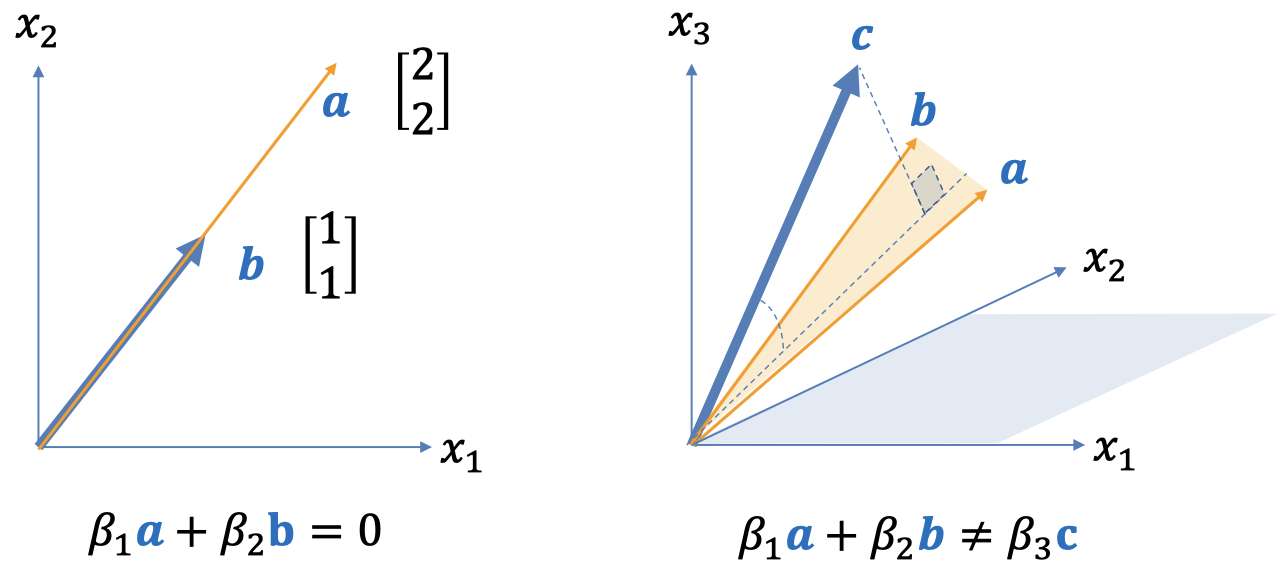
\includegraphics[width=0.70\linewidth]{image/gerolieanr.png}
    \end{figure}
    \item Matrix-vector notation : $\displaystyle \matr{Xw} = \matr{y}$ where \\
    $\matr{X} = \begin{bmatrix}
    x_{1,1} & x_{1,2} & \cdots & x_{1,d} \\
    \vdots & \vdots & \ddots & \vdots \\
    x_{m,1} & x_{m,2} & \cdots & x_{m,d}
    \end{bmatrix}$, $\matr{w} = \begin{bmatrix}
        w_1\\ \vdots \\ w_d
    \end{bmatrix}$, $\matr{y} = \begin{bmatrix}
        y_1\\ \vdots \\ y_m
    \end{bmatrix}$. \\
    Where $\matr{X}$ is the data matrix and $\matr{y}$ is target vector. We are usually asked to calculate $w$ which is the unknown vector of parameters. The rank($\matr{X}$) corresponds to the maximal number of linearly independent columns or rows of X.
\end{enumerate}
\textbf{Causality and Simpsons's paradox}
\begin{enumerate}
    \item Causality \\ 
    The influence by which one event or process contributes to another, The cause is partly responsible for the effect, and the effect is partly dependent on the cause.\\
    \textbf{Randomized Controlled Trial (RCT)}, A study design that randomly assigns participants into an experimental group or a control group.\\
    As the study is conducted, the only expected difference between two groups is the outcome variable being studied.
    \item Correlation \\
    Correlations are useful because they can indicate a predictive relationship that can be exploited in practice.
    \begin{figure}[h]
        \centering
        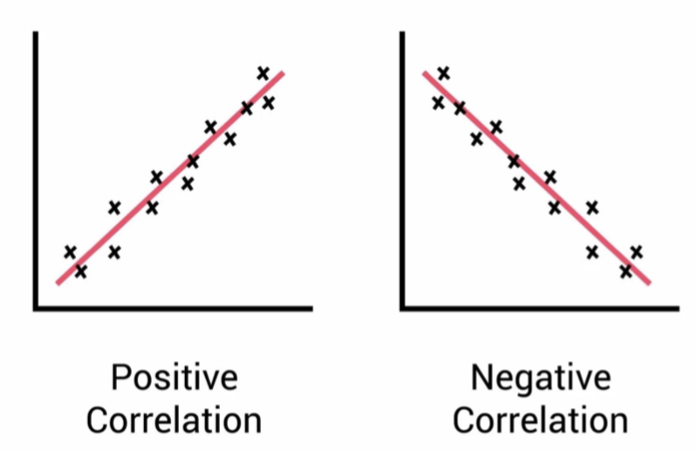
\includegraphics[width=0.75\linewidth]{image/correlation.png}
    \end{figure} \\
    Linear correlation coefficient, $r$, which is also known as \textit{near Pearson correlation Coefficient}. 
    \[r = \frac{\sum_{i=1}^{n} (x_i - \bar{x})(y_i - \bar{y})}
    {\sqrt{\sum_{i=1}^{n} (x_i - \bar{x})^2} \sqrt{\sum_{i=1}^{n} (y_i - \bar{y})^2}}
    = \frac{s_{xy}}{s_x s_y}\]
    \begin{table}[h]
        \centering
        \begin{tabular}{lc}
        \hline
        \textbf{Type of Relationship} & \textbf{Correlation Coefficient (\( r \))} \\
        \hline
        Strong linear relationship & \( r > 0.9 \) \\
        Medium linear relationship & \( 0.7 \leq r \leq 0.9 \) \\
        Weak linear relationship & \( 0.5 < r \leq 0.7 \) \\
        No or doubtful linear relationship & \( 0 < r \leq 0.5 \) \\
        \hline
        \end{tabular}
        \caption{Correlation coefficient and strength of linear relationship}
    \end{table}
    \item Simpson's paradox \\
    Simpson's paradox is a phenomenon in probability and statistics, in which a trend appears in several different groups of data but disappears or reverses when these groups are combined.
\end{enumerate}
\textbf{Random Variable, Bayes' Rule}
\begin{enumerate}
    \item Probability \\
    Sample space $S$, $A$ is a subset of $S$, named an event. \\
    Axioms of Probability
    \begin{enumerate}
        \item $P(A) \geq 0$
        \item $P(S) = 1$
        \item If $A \cap B = \emptyset$, then $P(A \cup B) = P(A) + P(B)$. Otherwise, $P(A \cup B) = P(A) + P(B) - P(A \cap B)$.
    \end{enumerate} 
    Take note in this particular course, use $Pr(\cdot)$ to represent probability symbol.
    \item Discrete Random Variable \\
    Expectation of DRV: \(E(x) \overset{\text{def}}{=} \sum_{i=1}^{k} [x_i \cdot \Pr(X = x_i)]\)
    where $Pr(X = x_i)$ is the probability that $X$ has the value $x_i$ acoording to the PMF.\\
    Standard deviation: \(\sigma \overset{\text{def}}{=} \sqrt{E\left[(X - \mu)^2\right]}\) \\
    Variance: \(\sigma^2 = E\left[(X - \mu)^2\right]\) \\
    \item Continuous Random Variable \\
    Expectation of CRV: \(E[X] \overset{\text{def}}{=} \int_{\mathbb{R}}\) \\
    Variance: \(\sigma^2 \overset{\text{def}}{=} \int_{\mathbb{R}} (X - \mu)^2 f_X(x) \, dx\) \\
    \item Two Basic Rules
    Sum rule
    \[\Pr(X = x) = \sum_{Y} \Pr(X = x, Y = y_i)\]
    Product rule
    \[\Pr(X = x, Y = y) = \Pr(Y = y | X = x) P(X = x)\]
    \item Bayes' Rule
    \[\Pr(Y = y | X = x) = \frac{\Pr(X = x | Y = y) \Pr(Y = y)}{\Pr(X = x)}\]
\end{enumerate}
\subsubsection{System of Linear Equations}
\textbf{Operations on vectors and Matrices}
\begin{enumerate}
    \item Transpose \\
    \[\matr{x} = \begin{bmatrix}
        x_1 \\
        x_2
    \end{bmatrix} \quad \matr{x}^T = \begin{bmatrix}
        x_1& x_2
    \end{bmatrix}\]
    In python you may use \texttt{numpy} to find out the tranpose or rank of the vector or matrix.
    \begin{minted}{python}
        import numpy as np
        from numpy.linalg import matrix_rank
        X = np.array([[1, 4, 3], [0, 4, 2], [1, 8, 5]]) 
        print(matrix_rank(X)) #Calculating Rank
        print(X)
        print(X.T) #This is the transpose of X
    \end{minted}
    
\end{enumerate}




\newpage
\section{Engineering}
\subsection{Principle of Electrical engineering}
\subsubsection{Electronic Components}
\begin{enumerate}
    \item \textbf{Capacitance} is a parameter that quantifies the amount of charge required to make one volt p.d across the plates.\\
\[C=\frac{q}{V}\]
The e field created by the separate of charge is:
\[E=\frac{q}{\epsilon A}\] 
\[\epsilon_0 =8.85\times10^12\ F/m\]
where $\epsilon = \epsilon_r \epsilon_0$, and $\epsilon_r$ is the relative permittivity of a given material. 
\[V=E\times d=\frac{qd}{\epsilon A}\]
where $d$ is the separation of the two plates, $\epsilon$ is the permittivity or dielectric constant.\\
Capacitance is :
\[C=\frac{q}{V}=\frac{\epsilon A}{d}\]
\[i_C = C\frac{dv_C}{dt}\]
Voltage in terms of Current:
\[q(t)=\int^t_{t_0}{i(t)\, dt+q(t_0)}\]
\[v(t)=\frac{1}{C}\int^t_{t_0}{i(t)\, dt+v(t_0)}\]
Stored Energy:
\[w(t)=\frac{1}{2}Cv^2(t)\]
\[w(t)=\frac{1}{2}v(t)q(t)\]
\[w(t)=\frac{q^2(t)}{2C}\]
Capacitance in parallel:
\[C_{eq} = C_1+C_2+C_3\]
Capacitance in series:
\[C_{eq}=\frac{1}{\frac{1}{C_1}+\frac{1}{C_2}+\frac{1}{C_3}}\]
Capacitor Voltage while being discharged:
\[v_{C}(t)=V_0e^{-\frac{t}{RC}}\]
The speed of discharging is determined by the product of R and C, this is known as the \textbf{time constant}: $\tau=RC$ for a RC circuit.\\
Usually it takes 5$\tau$ to fully charge or discharge a capacitor.\\
Capacitor Voltage while charging:
\[v_{C}(t)=V_S(1-e^{-\frac{t}{\tau}})\] when charging from 0 $V$.\\
Current discharged in Capacitor:
\[i_C(t)=\frac{V_s}{R}e^{-\frac{t}{RC}}\]
    \item \textbf{Inductor} stores energy in a circuit and the working principle of an inductor is based on magnetic effect of electric current.\\
\textbf{Magnetic Flux density} is the amount of magnetic flux passing through per unit area $B = \frac{\phi}{A}$, where, $\phi$ is the magnetic flux and $A$ is the area which flux passes.
Flux-linkage of a coil:
\[\Psi = N\phi\]
\[\Psi = Li\]
The constant proportionality of L is called \textbf{inductance}. The unit of inductance is Henry($H$). \\
\textit{Faraday's Law}, the magnitude of the induced voltage is equal to the rate of change of flux-linkage of the coil.
\[v_L=\frac{d\Psi}{dt}\]
Element law of inductor:
\begin{align*}
v_L &= \frac{dLi}{dt}\\
    &= L\frac{di}{dt}
\end{align*}
Current and voltage relationship in inductor:
\[i(t)=\frac{1}{L}\int^t_{t_0}v(t)dt+i(t_0)\]
instantaneous power of an inductor:
\[p_L =v_Li_L =L\frac{di_L}{dt}i_L\]
Stored Energy:
\[w(t)=L\int^{I}_{0}i_Ld_{iL} = \frac{1}{2}Li^2(t)\]
Inductors in parallel:
\[L_{eq}=\frac{1}{\frac{1}{L_1}+\frac{1}{L_2}+\frac{1}{L_e}}\]
Inductors in series:
\[L_{eq}=L_1+L_2+L_3\]
\end{enumerate}

\newpage
\subsection{Electronic Circuits}
\subsubsection{Basic Concepts}
\begin{enumerate}
    \item Voltage \& Current divider Rule\\
    \begin{circuitikz} [american]
        \draw
        (0,0)
            to[V, l=$V(t)$] (0,3)
            to[R, l=$Z_1$, v<=$V_1(t)$, i>^=$i(t)$] (3,3) % The voltage source and resistor Z1
            to[short, -*] (4,3)
            to[R, l=$Z_2$, i>^=$i_1(t)$] (4,0) % The resistor Z2
            to[short, -*] (3,0)
        (4,3) 
            to[short] (6,3)
            to[R, l=$Z_3$, v<=$V_3(t)$, i<=$i_2(t)$] (6,0) % The resistor Z3
            to[short] (4,0)
        (3,3) 
            to[open, v^>=$V_2(t)$] (3,0) % The open circuit for voltage V2(t)
        (0,0) 
            to[short] (6,0)
        ;
        \draw [dashed] (2.5,3.5) rectangle (7.0,-0.5) node[above right] {$Z_{\text{Total}}$};
        \draw (3,-1) node {$\frac{1}{Z_{\text{Total}}} = \frac{1}{Z_2} + \frac{1}{Z_3}$};
    \end{circuitikz}\\
    For Voltages:
    \begin{align*}
        V(t) &= V_1(t) + V_2(t) \\
        V_1(t) &= \frac{Z_1(t)}{Z_1(t) + Z_{\text{Total}}(t)} V(t) \\
        V_2(t) &= \frac{Z_{\text{Total}}(t)}{Z_1(t) + Z_{\text{Total}}(t)} V(t)
    \end{align*}
    For Currents:
    \begin{align*}
    I(t) &= I_1(t) + I_2(t) \\
    I_1(t) &= \frac{Z_3(t)}{Z_2(t) + Z_3(t)} I(t) \\
    I_2(t) &= \frac{Z_2(t)}{Z_2(t) + Z_3(t)} I(t)
    \end{align*}
    \item Node Analysis KCL
    \begin{center}
    \begin{circuitikz}[american]
    \draw(0,1) to [short, -*, i=$i_y$](0,0);
    \draw(-1,0) to [short, -*, i=$i_x$](0,0);
    \draw (1,0) to [short, -*, i=$i_z$](0,0);
    \end{circuitikz}
    \end{center}
    Currents flowing into a network sum to zero. Since current $i$ is equal to the rate of flow of charge $q$ that $i = \frac{dq}{dt}$, KCL corresponds to the conservation of charge. You can view KCL as a netwrok, and all currents flow into the network sums to zero.\\
    \begin{exam}
    $\;$
    \begin{figure}[h]
        \centering
        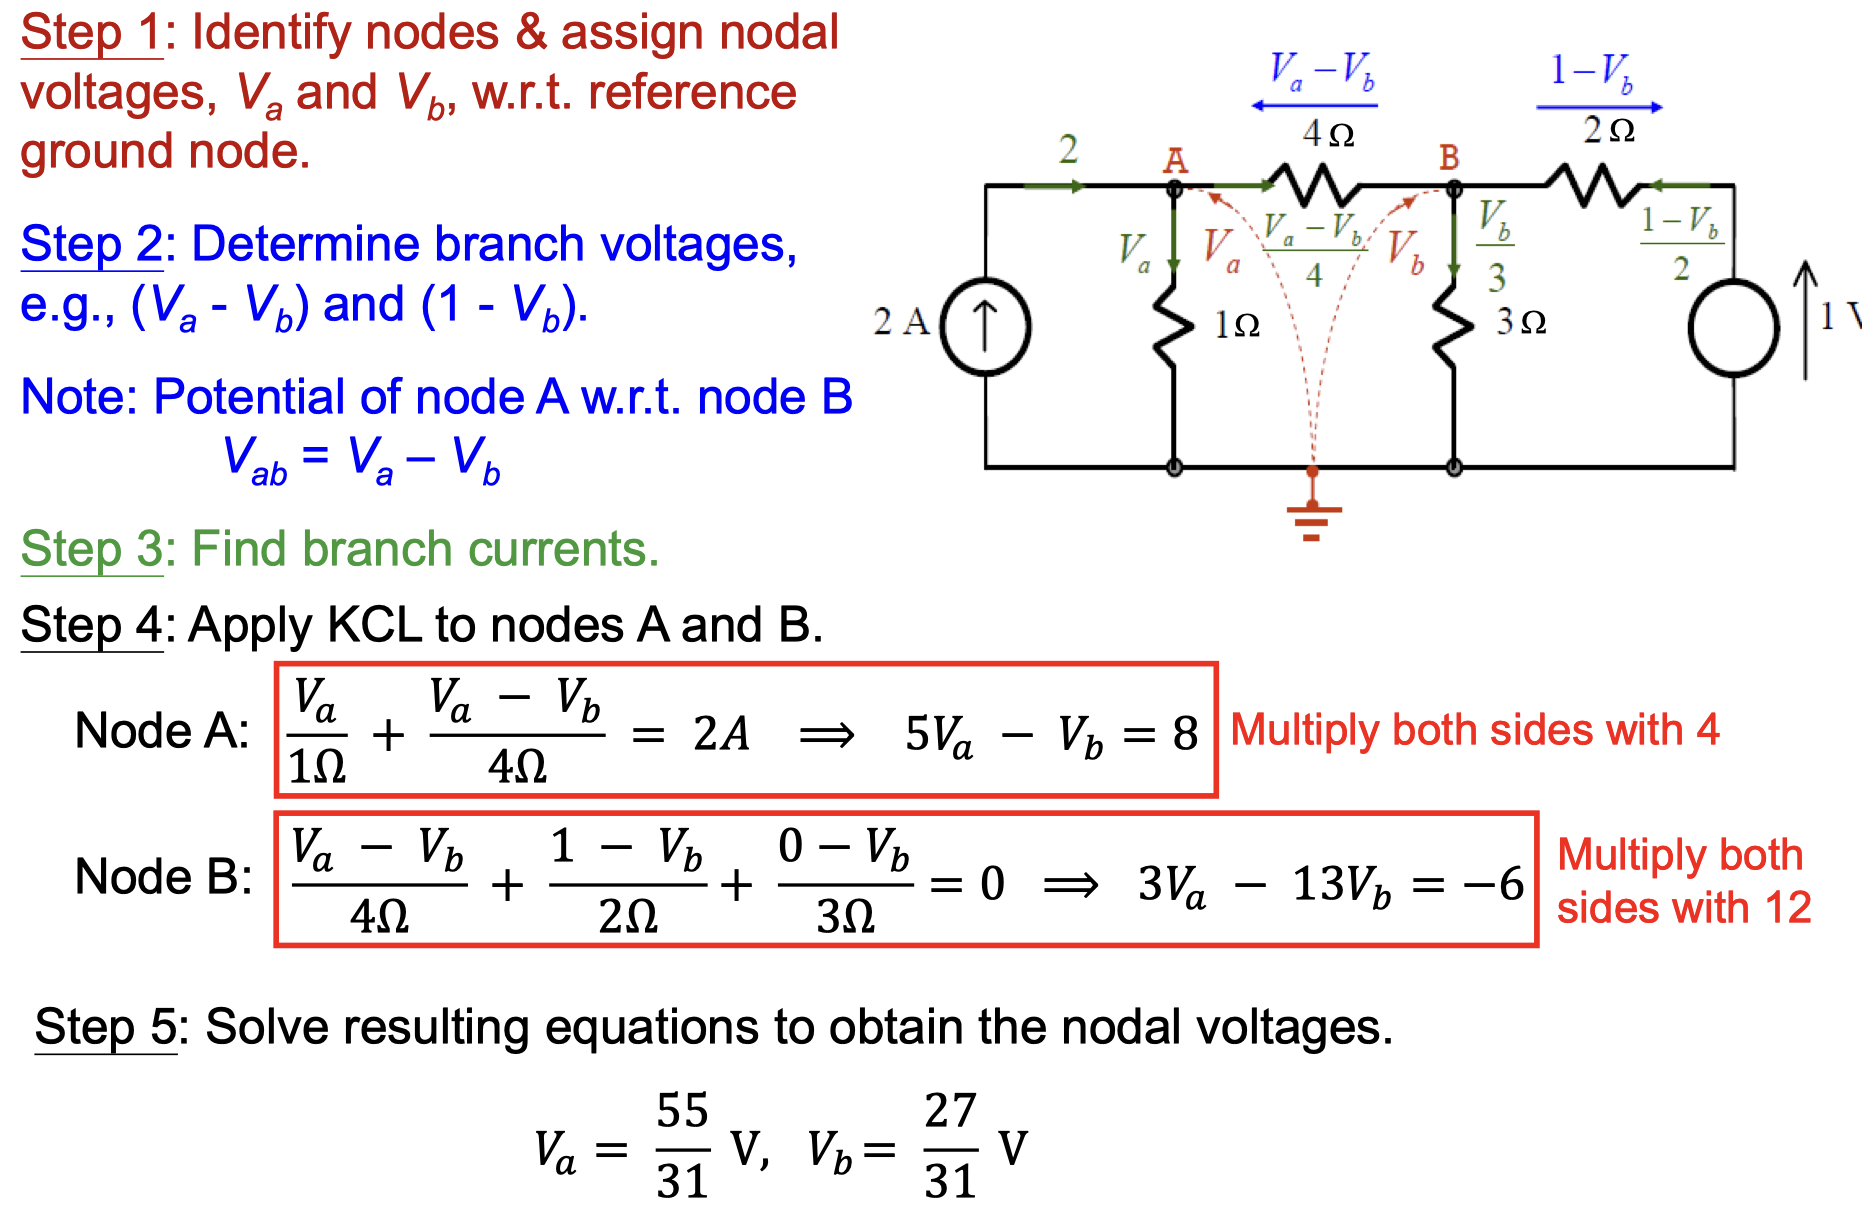
\includegraphics[width=0.75\linewidth]{image/KCL.png}
    \end{figure}
    \end{exam}
    \item Mesh Analysis KVL \\
    The sum of potential differences around any closed-loop is zero.
    \begin{center}
    \begin{circuitikz}[american]
        \draw (0,0) node[ground]{} to [battery2, invert, v=$V_A$] (0,2) -- (0,3)to  [R , R = $R_1$, v=$V_{R1}$] (3,3) to (3,3) to [R, R=$R_2$, v=$V_R2$](3,1) to [isource, l=$I_B$, v=$V_{IB}$](3,0) to node[ground]{} (3,0);
        \draw (3,3) to (5,3) to [R, R=$R_3$, v=$V_R3$](5,1) -- (5,0) to node[ground]{} (5,0);
    \end{circuitikz}
    \end{center}
    Loop 1: $V_A + (-V_{R1})+(-V_(R2))+(-V_{IB}) = 0$ \\
    Loop 2: $V_{IB}+V_{R2}+(-V_{R3}) = 0$\\
    Loop 3: $V_A + (-V_{R1})+(-V_{R3}) = 0$
    \item Linear Superposition \\
    When determining the impact of an individual source, you need to kill all other voltage source by short-circuiting them, and all other current source by open-circuiting them.
    \begin{figure}[h]
        \centering
        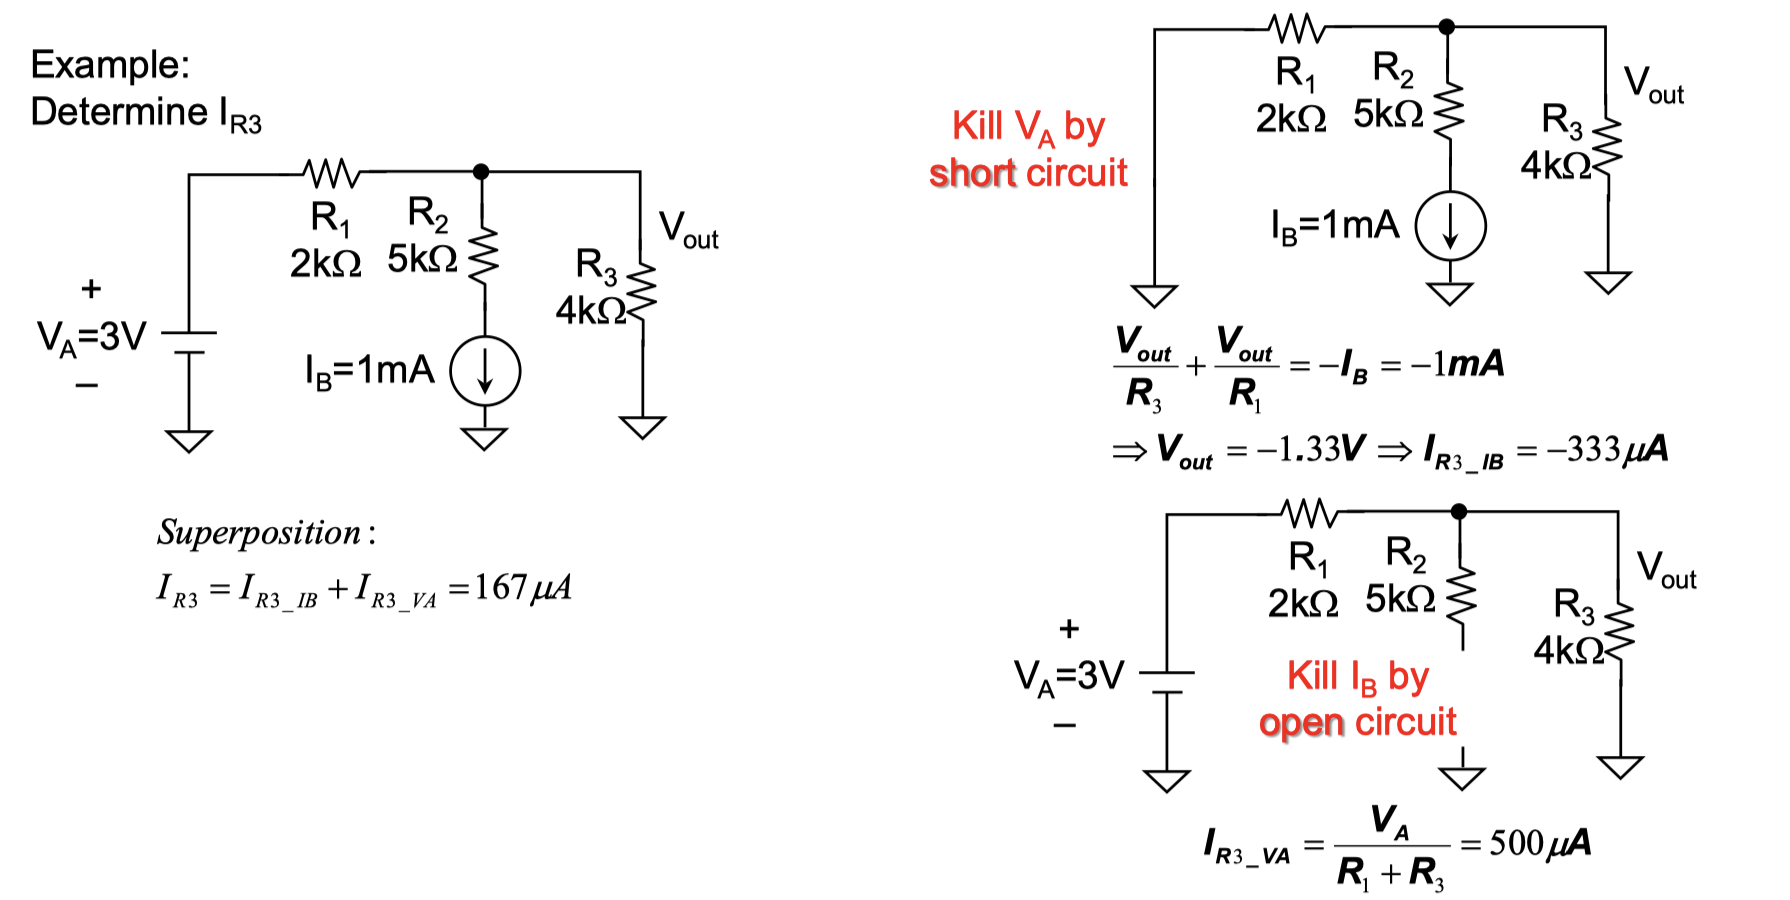
\includegraphics[width=0.8\linewidth]{image/linearsuper.png}
    \end{figure}
    \item Thevenin \& Norton Equivalent \\
    Thevenin Theorem: Any linear network with one port output can be replaced with an equivalent Thevenin voltage source $V_{THV}$ in series with a Thevenin resistance $R_{THV}$. \\
    Steps for Thevenin theorem :
    \begin{enumerate}
        \item Replace the port as an open circuit.
        \item Replace independent voltage source with short-circuit.
        \item Replace independent current source with open circuit.
        \item Calculate the $R_{THV}$ of the circuit.
        \item Calculate the $V_{THV}$ at the open port
        \item Re-draw the circuit with $V_{THV}$, $R_{THV}$ and $R$ at the open port to calculate $i$.
        \item $i$ will be the current flowing through your open port.
    \end{enumerate}
    Norton Theorem: \\
    Any linear network with one port output can be replaced with an equivalent Norton current source $I_{NOR}$ in parallel with a Norton resistance $R_{NOR}$.
    Steps for Norton theorem:
    \begin{enumerate}
        \item Replace the port as an open circuit.
        \item Replace independent voltage source with short-circuit.
        \item Replace independent current source with open circuit.
        \item Calculate the $R_{NOR}$ of the circuit.
        \item Calculate the $V_{THV}$ at the open port
        \item Calculate the $I_{NOR} = \frac{V_{THV}}{R_{NOR}}$.
        \item Re-draw the circuit with $I_{NOR}$, $R_{NOR}$ and $R_{load}$ as below to calculate $I_{load}$.
        \begin{center}
        \begin{circuitikz}[american]
            \draw (0,0) to [isource, l=$I_{NOR}$](0,3) to [short,-*](2,3) to [R,R=$R_{VOR}$](2,0) to (0,0);
            \draw (2,3) to [short, i=$I_{load}$](4,3) to [R, R=$R_{load}$](4,0) to [short,-*](2,0);
        \end{circuitikz}
        \end{center}
    \end{enumerate}
    \item AC Signal Quantities
    \begin{enumerate}
        \item Average value for AC signal
        \[v_{avg} = \frac{1}{T}\int^T_0v(t)dt\]
        \item Root-Mean-Square for AC
        \[v_{rms} = \sqrt{\frac{1}{T}\int^T_0v^2(t)dt}\]
    \end{enumerate}
    \item Phasor \\
    For AC Sinusoidal function \\
    Phasor $\underbrace{V = re^{j\theta} = r \angle \theta}_{\text{r is r.m.s}}$
    \item Capacitor
    \[i(t) = C\frac{dv(t)}{dt}\]
    Treat capacitor as open circuit in DC circuit analysis.\\
    Reactance of capacitor: $\displaystyle X_C = \frac{1}{j\omega C}$ \\
    Laplace Transformation: $\displaystyle V_C(s) = \frac{I(s)}{sC} \hspace{1cm} Z_C(s)=\frac{1}{sC}$ 
    \item Inductor
    \[v(t) = L\frac{di(t)}{dt}\]
    Treat inudctor as a short circuit in DC circuit analysis.\\
    Reactance of inductor: $\displaystyle X_L = j\omega L$ \\
    Laplace Transformation: $V_L(s)=sLI(s) \hspace{1cm} Z_L(s)=sL$
    \item Impedance and Admittance\\
    Impedance: Resistance + Reactance
    \[Z = R + jX\]
    Admittance: Conductance + Susceptance
    \begin{align*}
        Y &= \frac{1}{Z} = G +j B \\
        G &= \frac{R}{R^2 + X^2} \\
        B &= \frac{-X}{R^2 + X^2}\\
    \end{align*}
    \item RC Circuits \\
    Passive $1^{st}$ Order Low Pass Filter
        \begin{center}
            \begin{circuitikz}
                \draw
                (0,0)
                to[R, l=$R_1$, o-] (3,0)
                -- (3,-0.5)
                to[C, l=$C_1$] (3,-2)
                node[ground]{}
                (3,0)
                to[short, -o] (4,0)
                node[right] {$V_{\text{out}}$}
                (0,0)
                node[left] {$V_{\text{in}}$};
            \end{circuitikz}
        \end{center}
        $\displaystyle H(j\omega) = \frac{V_{\text{out}}}{V_{\text{in}}} = \frac{\frac{1}{j\omega C_1}}{\frac{1}{j\omega C_1} + R_1} = \frac{1}{j\omega C_1 R_1 + 1}$\\
        $3dB$ Gain \\
        \begin{enumerate}
            \item Since $\displaystyle |H(j\omega_{3dB})| = \frac{1}{\sqrt{2}}$ \\
            \item $\displaystyle \frac{1}{\sqrt{(\omega_{3dB}R_1C_1)^2+1}} = \frac{1}{\sqrt{2}}$  \\
            \item $\displaystyle \omega_{3dB} = \frac{1}{R_1C_1} $ \\
            \item $\displaystyle f_{3dB} = \frac{1}{2\pi R_1C_1}$
        \end{enumerate}
        \pagebreak
        Passive $1^{st}$ Order High Pass Filter
        \begin{center}
            \begin{circuitikz}
                \draw
                (0,0)
                to[C, l=$C_1$, o-] (3,0)
                -- (3,-0.5)
                to[R, l=$R_1$] (3,-2)
                node[ground]{}
                (3,0)
                to[short, -o] (4,0)
                node[right] {$V_{\text{out}}$}
                (0,0)
                node[left] {$V_{\text{in}}$};
            \end{circuitikz}
        \end{center}
        $\displaystyle H(j\omega) = \frac{V_{\text{out}}}{V_{\text{in}}} = \frac{R_1}{\frac{1}{j\omega C_1} + R_1} 
        = \frac{j\omega C_1 R_1}{j\omega C_1 R_1 + 1} = \frac{j\omega}{j\omega + \frac{1}{C_1 R_1}}$\\
        $3dB$ Gain\\
        Same logic as above, $\displaystyle f_{3dB} = \frac{1}{2\pi R_1C_1}$
        \item Maximum Power Transfer
        \begin{figure}[h]
            \centering
            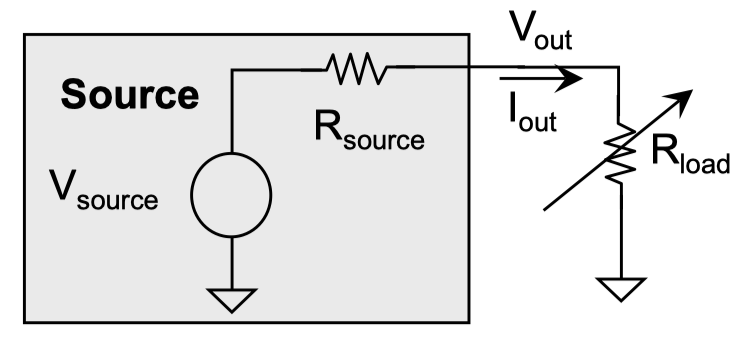
\includegraphics[width=0.75\linewidth]{image/powersource.png}
        \end{figure}
        \begin{align*}
        P_{\text{out}} &= \frac{V_{\text{source}}}{R_{\text{source}} + R_{\text{load}}} \times \frac{R_{\text{load}} V_{\text{source}}}{R_{\text{source}} + R_{\text{load}}} \\
        &= \frac{R_{\text{load}} V_{\text{source}}^2}{(R_{\text{source}} + R_{\text{load}})^2} \\
        \frac{dP_{\text{out}}}{dR_{\text{load}}} &= \frac{1}{(R_{\text{source}} + R_{\text{load}})^2} - \frac{2R_{\text{load}}}{(R_{\text{source}} + R_{\text{load}})^3} = 0 \\
        \Rightarrow R_{\text{load}} &= R_{\text{source}}
        \end{align*}
        Therefore, We can conclude that the maximum power transfer occurs when the $R_{\text{load}} = R_{\text{source}}$.
        \item Transients RC Circuits\\
        The transient state of a circuits is right after the circuit being switched on or off before reaching the steady state.
        \begin{exam}
            Here is a typical example.
            \begin{figure}[h]
                \centering
                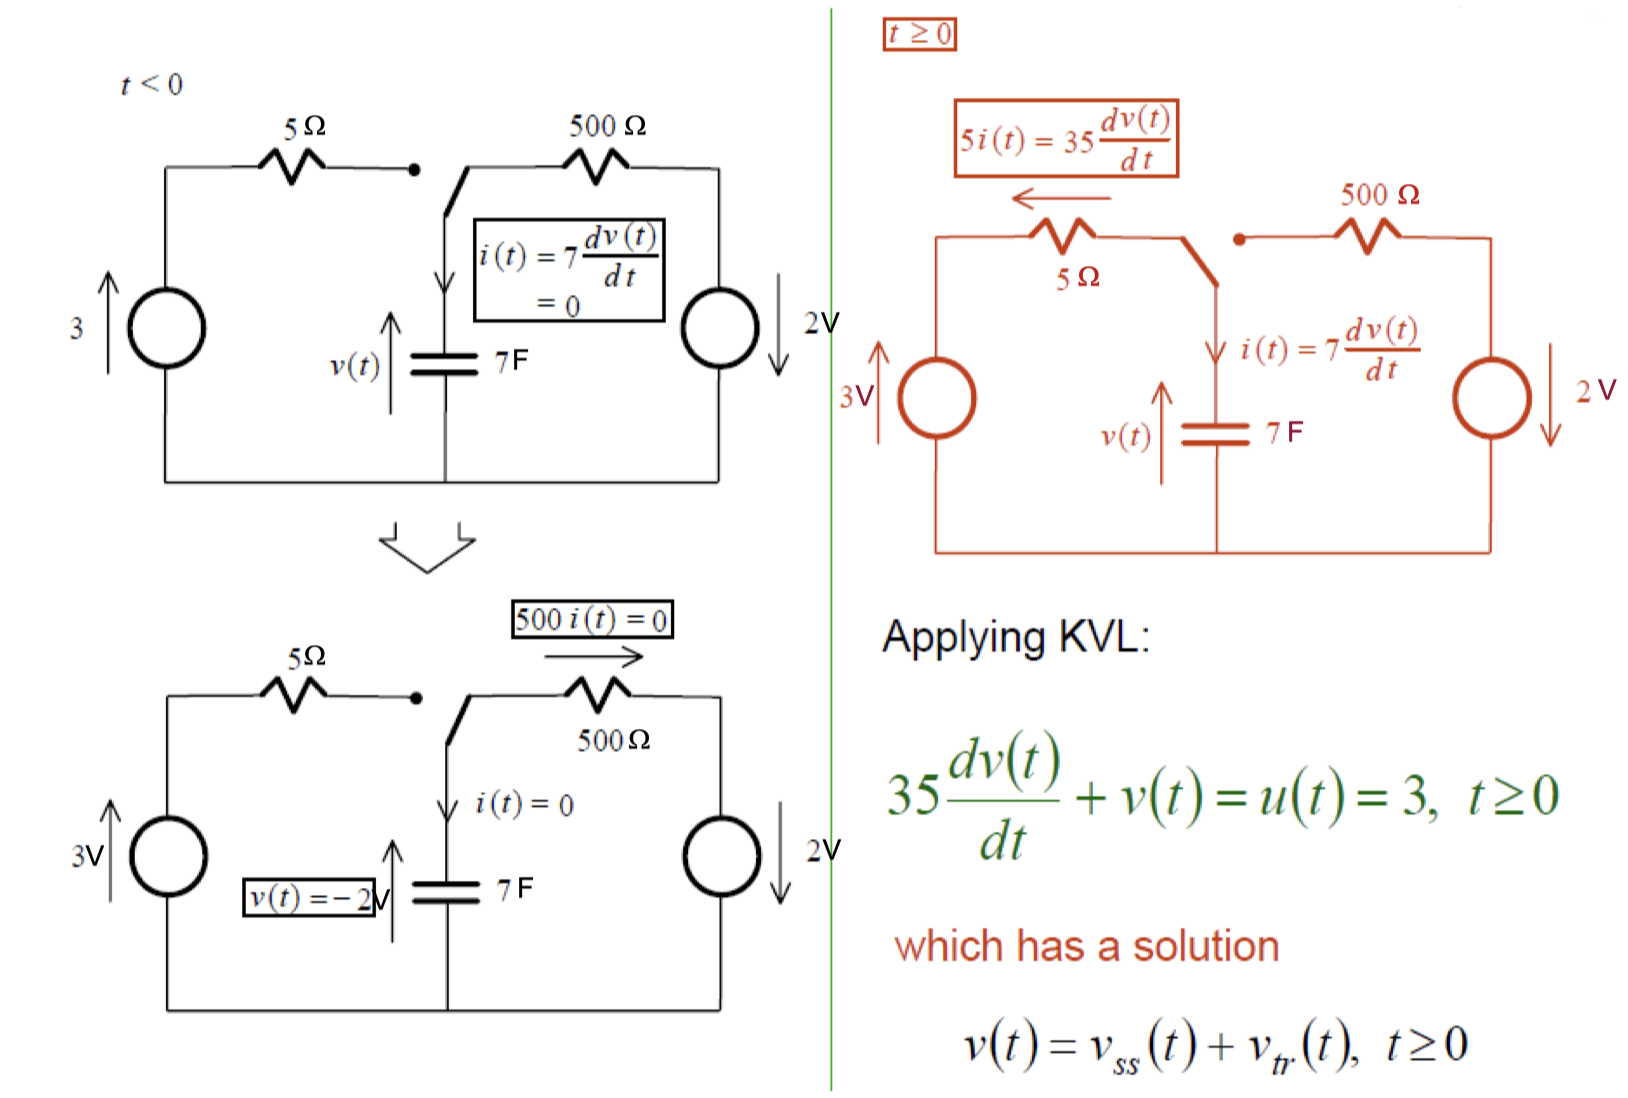
\includegraphics[width=0.75\linewidth]{image/transient.png}
            \end{figure}
        \end{exam}
        \item Power (instantaneous and average)
        \begin{figure}[h]
            \centering
            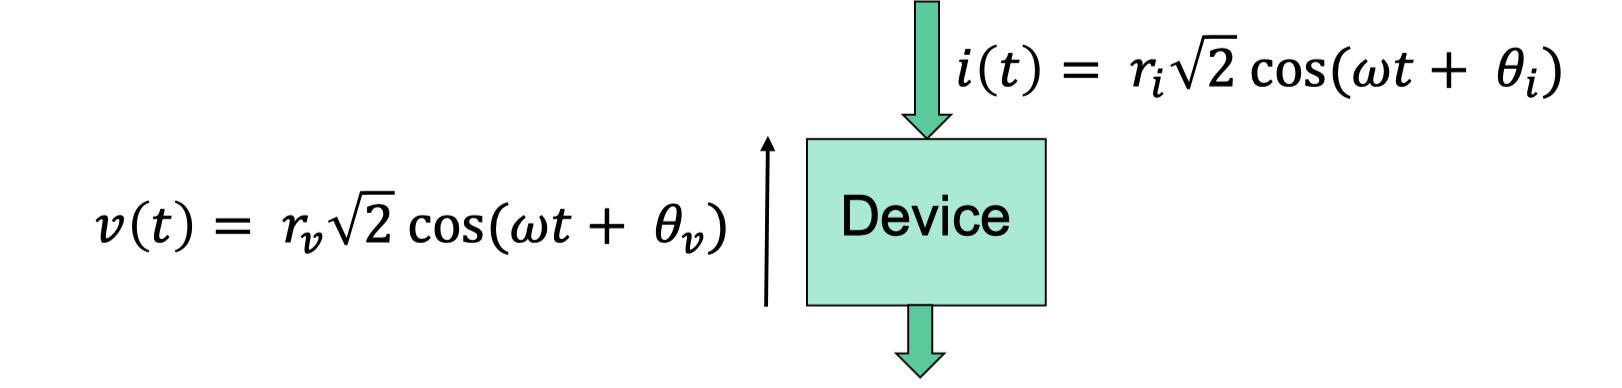
\includegraphics[width=0.75\linewidth]{image/poweri.png}
        \end{figure}\\
        For a given device, the instantaneous power can be derived in 
        \begin{align*} 
        p(t) & = i(t)v(t) \\
        &= 2r_ir_v \cos(\omega t + \theta_i) \cos(\omega t + \theta_v)\\ 
        &= r_ir_v(\cos(\theta_i - \theta_v) + \cos(2\omega t + \theta_i + \theta_v)) \\
        \end{align*} 
        Note the change from line 2 to line 3 is because $2 \cos(x_1) \cos(x_2) = \cos(x_1 - x_2) + \cos(x_1 + x_2)$
        \newpage
        The average power is 
        \begin{align*}
        P_{\text{av}} &= \frac{1}{T} \int_{0}^{T} p(t) dt \\
        &= \frac{r_i r_v}{T} \int_{0}^{T} \left[ \cos(\theta_i - \theta_v) + \cos\left(\frac{4\pi t}{T} + \theta_i + \theta_v\right) \right] dt \\
        &= r_i r_v \cos(\theta_i - \theta_v), \quad \text{where } T = \text{Period and } \omega = \frac{2\pi}{T} \\
        &= r_v r_i \cos(\theta_v - \theta_i) \\
        &= \Re\{r_v r_i e^{j(\theta_v - \theta_i)}\} \\
        &= \Re\{r_v r_i e^{j(\theta_i - \theta_v)}\} \\
        &= \Re\{V^* I\} \\
        &= \Re\{VI^*\} \\
        \end{align*}
        \item Power Factor
        \begin{enumerate}
            \item $\text{Real Power (Average)} = \Re[V^*I] = r_vr_i\cos(\theta_i-\theta_v)$
            \item  $\displaystyle \text{Apparent Power} = |V||I| = r_vr_i$
            \item Thus, $\displaystyle \text{Power Factor} = \frac{\text{Real Power}}{\text{Apparent Power}} = \cos(\theta_i-\theta_v)$ 
            \item When $V$ and $I$ are in phase, $\theta_i = \theta_v$ , power factor is unity.
            \item Leading Power Factor: $I$ leads $V$ where $\theta_i > \theta_v$ .
            \item Lagging Power Factor: $I$ lags $V$ where $\theta_i < \theta_v$.
        \end{enumerate}
\end{enumerate}
\subsubsection{Diode (pn-Junction)}
\begin{enumerate}
    \item Introduction
    \begin{enumerate}
        \item The diode to be discussed is a semiconductor pn-junction. Please see this \href{https://www.youtube.com/watch?v=Fwj_d3uO5g8}{link} before reading notes.
        \item p-type (\textbf{Holes}) impurity is a group \rom{3} elements (\ce{Br},\ce{Al},\ce{Ga})\\
        n-type (\textbf{Electrons}) impurity is a group \rom{5} elements (\ce{P},\ce{As},\ce{Sb})
        \item The process of doping can also change a p-type semiconductor to n-type semiconductor, and vice versa.
        \item Two types of charge carrier movement namely, drift and diffusion.
        \begin{enumerate}
            \item Drift current $I_{Drift}$ : Charge carriers move in the presence of electric field.
            \item Diffusion Current $I_{Diffusion}$ : Charge carriers diffuse owing to the difference in carrier concentration.
        \end{enumerate}
        \item IV Characteristic\\
            \begin{minipage}{0.4\textwidth}
            It allows current flow through it easily in one direction (forward direction), but not opposite directions (reverse direction), except for the reverse breakdown region.
            \end{minipage}
            \begin{minipage}{0.6\textwidth}
                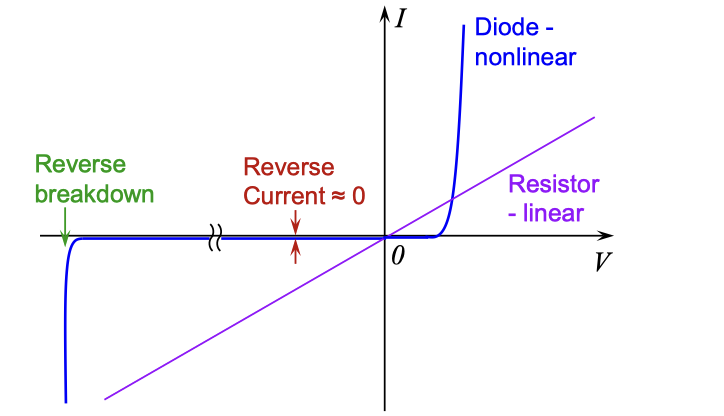
\includegraphics[width=1\linewidth]{image/pnchar.png}
            \end{minipage}
    \end{enumerate}
    \item Forward-Bias \\
    \\
    \begin{minipage}{0.4\textwidth}
        Under forward-bias, the p-type terminal is at a higher voltage with respect to the n-type terminal. \\
        The forward current remains small $\approx 0$ until the cut-in voltage and increases quickly with a small increase in $V$. \\
        The voltage drop across the diode lies in a narrow range.
    \end{minipage}
    \begin{minipage}{0.6\textwidth}
        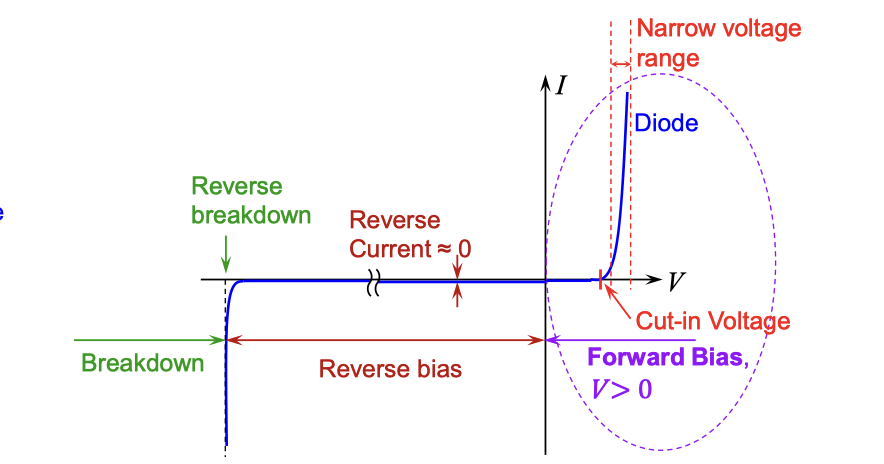
\includegraphics[width=1\linewidth]{image/diodeforawd.png}
    \end{minipage}
    \item Reverse-Bias \\
    \\
    \begin{minipage}{0.4\textwidth}
        Under reverse-bias $V<0$, an external voltage is applied such that the p-type terminal is at a lower voltage with respective to the n-type terminal. \\       
        For $\displaystyle |V| = V_R < V_Z$, the breakdown voltage reverse current is very small and can be treated as 0.
    \end{minipage}
    \begin{minipage}{0.6\textwidth}
        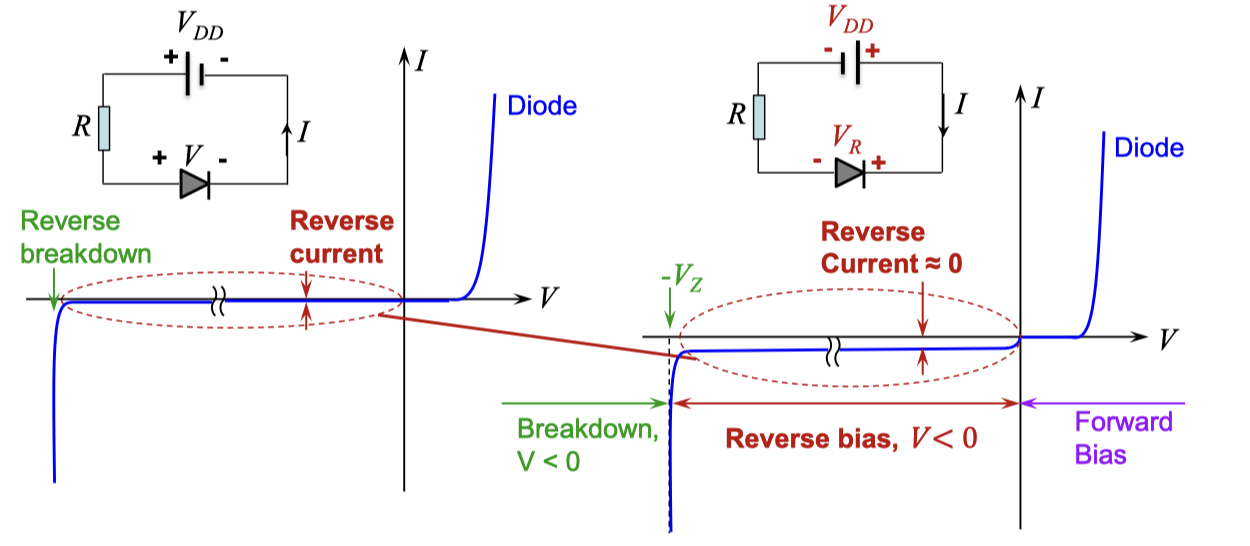
\includegraphics[width=1\linewidth]{image/reversebias.png}
    \end{minipage}
    \item Breakdown Region\\
    \\
    \begin{minipage}{0.4\textwidth}
        When $\displaystyle V_{DD} > V_Z$, the current can be very large, while its voltage is practically not changed and stays at $-V_Z$. This is called \textbf{Breakdown}\\
        The current can be limited by connecting a resistor $R$ in series with the pn junction diode. $\displaystyle I = \frac{V_{DD}-V_Z}{R}$
    \end{minipage}
    \begin{minipage}{0.6\textwidth}
        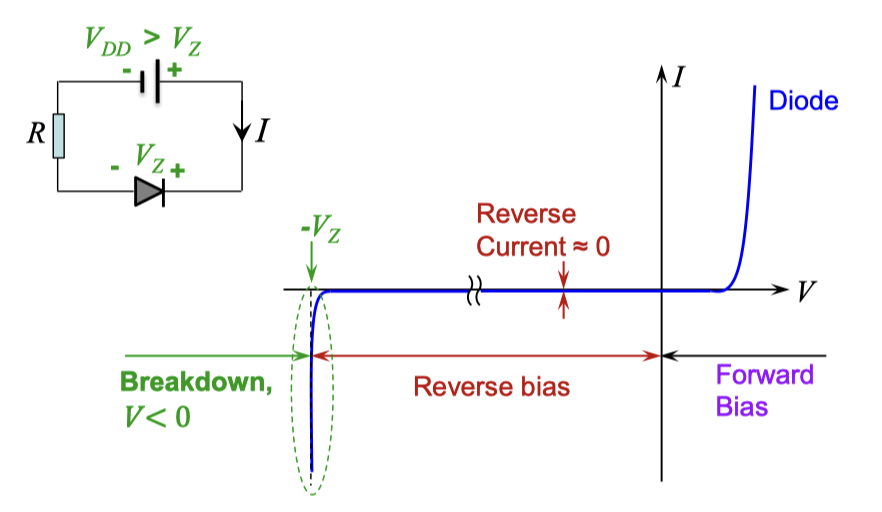
\includegraphics[width=1\linewidth]{image/breakdownregion.png}
    \end{minipage}
    \item Current Voltage Characteristic
    \[I = I_S(e^{\frac{V}{nV_T}}-1)\]
    \begin{enumerate}
        \item $V$ is the voltage across the diode.
        \item  $I$ is the current flowing through the diode.
        \item $V_T$ is thermal voltage, $\displaystyle V_T = \frac{kT}{q} = 0.0259V \approx 0.025V \approx 0.026V$ at $T = 300K$.
        \item $n$ is exponential factor between 1 and 2, where $n = 1$ is for an ideal pn-junction diode.
        \item $I_S$ is reverse saturation current, increases with increasing temperature.
    \end{enumerate}
    In substantial \textbf{Forward-Bias} ($V>$ cut-in voltage $> 0$), and $\displaystyle e^{\frac{V}{nV_T}} >> 1$ and therefore
    \[I = I_S(e^{\frac{V}{nV_T}}-1) \approx I_S e^{\frac{V}{nV_T}}\quad \text{or} \quad V\approx nV_T\ln(\frac{I}{I_S})\]
    $I \approx 0$ for $V < ~0.5V$, this is the cut-in voltage.\\
    The voltage drop across diode is around $0.6V$ to $0.8V$, usually we take as $0.7V$.\\
    In \textbf{Reverse-Bias} $V<0$, for $|V|>$ a few times $nV_T$ and $\displaystyle e^{\frac{V}{nV_T}} << 1$ and therefore
    \[I = I_S(e^{\frac{V}{nV_T}}-1) \approx -I_S\]    
    \newpage
    \item Large Signal Model
    \begin{figure}[h]
        \centering
        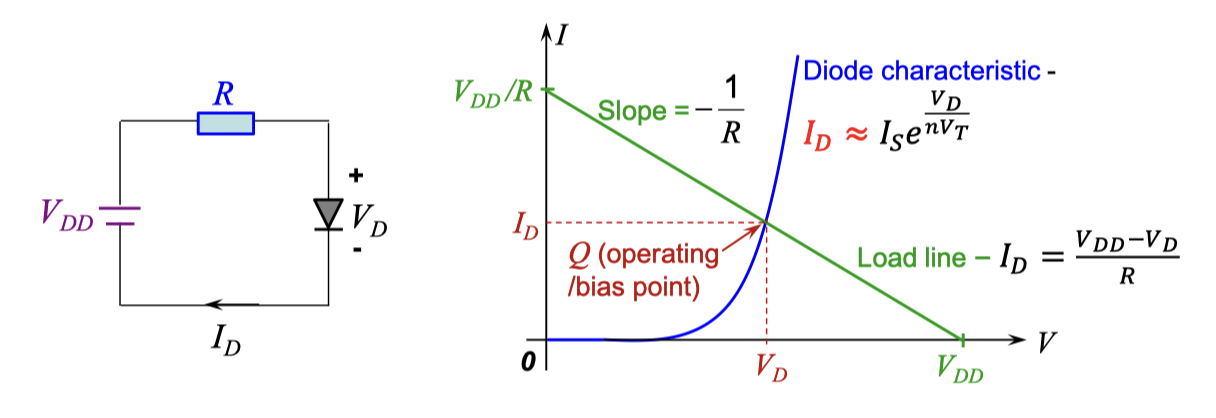
\includegraphics[width=1\linewidth]{image/largemodel.png}
    \end{figure} \\
    For a diode in forward-bias, assuming $\displaystyle V_{DD}>0.5V$ the IV characteristic is
    \[I_D \approx I_S e^{\frac{V_D}{nV_T}}\]
    $\displaystyle I_d \text{and} V_D$ are also governed by KVL where 
    \[I_D = \frac{V_{DD}-V_D}{R}\]
    Since, $I_D$ and $V_D$ cannot be determined easily by solving equations above. The can be solved graphically, or by iterative procedure. \\
    Here are the example of a circuit with \(nV_T = 0.043\) \\
    \begin{enumerate}
        \item We first assume \( V_D = V_{D0} = 0.7 \, \text{V} \).
        \item Next, substitute \( V_D = V_{D0} = 0.7 \, \text{V} \) into equation the KVL equation, we make an initially estimate for \(I_{D0} = \frac{V_{DD} - V_{D0}}{R} = \frac{5 - 0.7}{1000} = 4.3 \, \text{mA} \)
        \item Using the estimated \( I_{D0} = 4.3 \, \text{mA} \), a better estimate for \( V_D ( = V_{D1} ) \) is obtained using the diode equation
        \[ V_D - 0.6 \, \text{V} = nV_T \ln(\frac{I_D}{I_{1} mA}) \Rightarrow V_{D1} - 0.6 \, \text{V} = 0.043 \ln(\frac{4.3 \, \text{mA}}{1 \, \text{mA}}) \]
        \[ \Rightarrow V_{D1} = 0.6627 \, \text{V} \]
        \item Substitute \( V_{D1} = 0.6627 \, \text{V} \) into equation, a better estimate for \( I_D ( = I_{D1} ) \) is obtained
        \[ I_{D1} = \frac{V_{DD} - V_{D1}}{R} = \frac{5 - 0.6627}{1000} = 4.3373 \, \text{mA} \]
        \item Thus, after the 1st iteration \( I_{D1} = 4.3373 \, \text{mA} \) and \( V_{D1} = 0.6627 \, \text{V} \). The 2nd iteration proceeds in a similar manner, by repeating steps 3 and 4:
        \[ V_{D2} - 0.6 \, \text{V} = 0.043 \ln(\frac{4.3373 \, \text{mA}}{1 \, \text{mA}}) \Rightarrow V_{D2} = 0.6631 \, \text{V} \]
        \[ I_{D2} = \frac{V_{DD} - V_{D2}}{R} = \frac{5 - 0.6631}{1000} = 4.3369 \, \text{mA} \]
        \item 2nd iteration yields \( I_{D2} = 4.3369 \, \text{mA} \) and \( V_{D2} = 0.6631 \, \text{V} \), which are close to values obtained after the 1st iteration (less than 0.06\% difference), hence further iterations are not necessary, as the values of \( V_D \) and \( I_D \) have converged.
    \end{enumerate}
    As such, in order for easier calculation, we need to model diode.\\
    \begin{figure}[h]
        \centering
        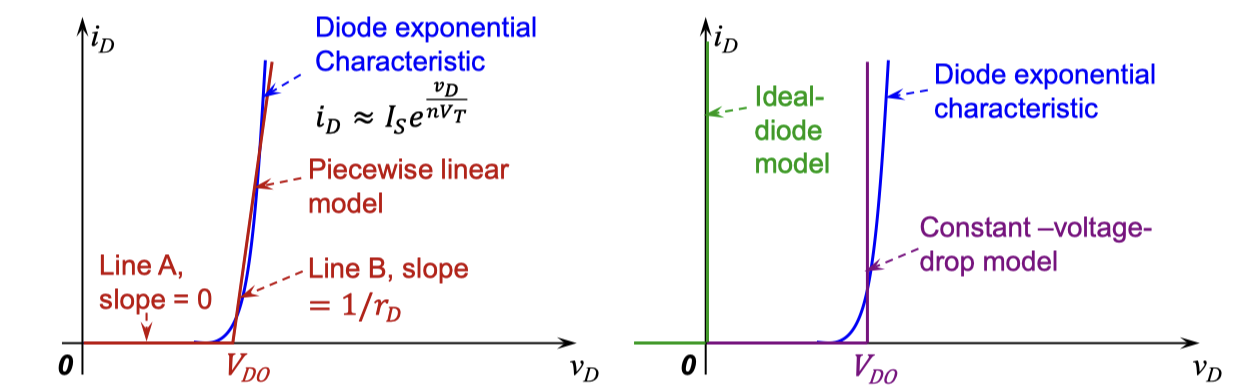
\includegraphics[width=1\linewidth]{image/largemodeling.png}
    \end{figure}
    \begin{enumerate}
        \item Piecewise-linear model: \(i_D = 0,\; \text{for}\; v_D\leq V_{D0}\) \\
        \(i_D = \frac{v_D - V_{D0}}{r_D}, \text{for} \; v_D \geq V_{D0}\)
        \item Ideal-diode model: \(V_{D0} = 0, \; r_D = 0\)
        \item Constant-voltage-drop model: \(r_D = 0, V_{D0} \; \text{is taken as} \; 0.7V.\) \\
        In constant-voltage-drop model, treat diode as a $0.7V$ drop and then calculate the rest.
    \end{enumerate}
    \newpage
    \item Small Signal Model \\
    This model are used with circuits with time varying signal (AC) in addition to the DC supply as shown in the graph below.
    \begin{figure}[h]
        \centering
        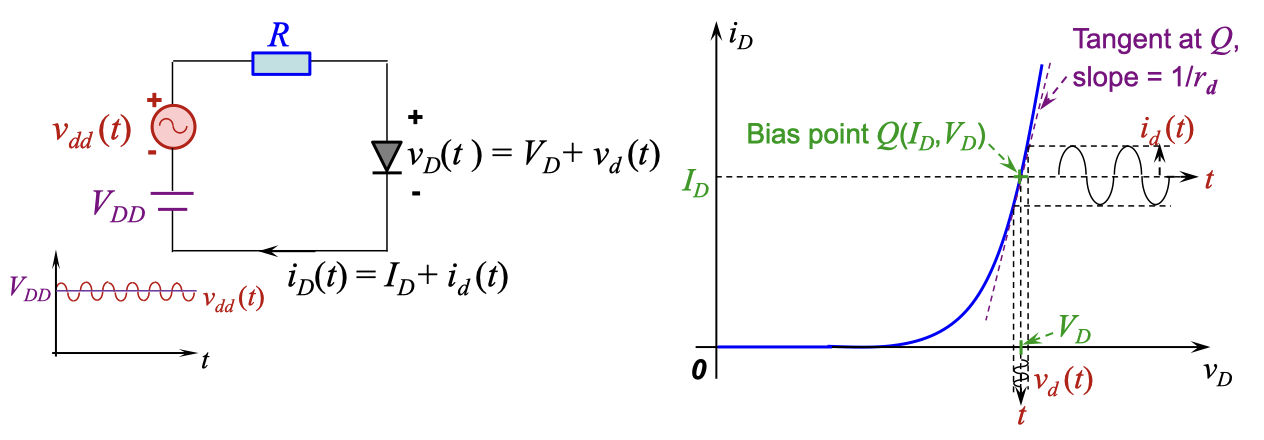
\includegraphics[width=1\linewidth]{image/smallsignalmodel.png}
    \end{figure}\\
    Calculation for such signal can be derived into two parts.
    \begin{enumerate}
        \item DC analysis, consider only $V_{DD}$, 
        \item AC analysis, consider only $v_{dd}(t)$
        \item Last, using superposition to give the total effect.
    \end{enumerate}
    Small-Signal Operation:
    \begin{enumerate}
        \item Find $I_D$ and $V_D$ using Large Signal Model.
        \item With a small signal source $v_{dd}(t)$
        \[i_D(t) = I_S e^{\frac{v_D(t)}{nV_T}} = I_S e^{\frac{V_D + v_d(t)}{nV_T}} = I_S e^{\frac{V_D}{nV_T}} e^{\frac{v_d(t)}{nV_T}} = I_D e^{\frac{v_d(t)}{nV_T}}\]
        \[\approx I_D[1+\frac{v_d(t)}{nV_T}] = I_D + \frac{I_D}{nV_T}v_d(t)\]
        Note, {\color{red}{\(e^x \approx 1 + x\)}} for $x < 1$ .
        \item Hence, $\displaystyle i_d(t) = \frac{I_D}{nV_T}v_d(t) = \frac{1}{r_d}v_d(t)$
        \item \(r_d = \frac{nV_T}{I_D}\), $r_d$ is called diode small-signal resistance.
        \item Since $r_d$ having a unit as $\Omega$, You can model the diode as a small resistor.
        \item \(i_d(t) = \frac{v_{dd}(t)}{R+r_d}\), Using KVL we can obtain the small-signal current.
        \item The slope at the DC bias point Q, givese the approximatelt the inverse of diode small-signal resistance $r_d$
        \[\frac{\partial i_D}{\partial v_D} \bigg|_{v_D = V_D} = \frac{1}{r_d} = \frac{i_d}{v_d} = \frac{I_D}{nV_T}\]
        \item $r_d$ is also known as the diode incremental resistance.
    \end{enumerate}
    \item Rectifier and Voltage Regulator\\
    Half-way Rectifier\\
    \begin{figure}[h]
        \centering
        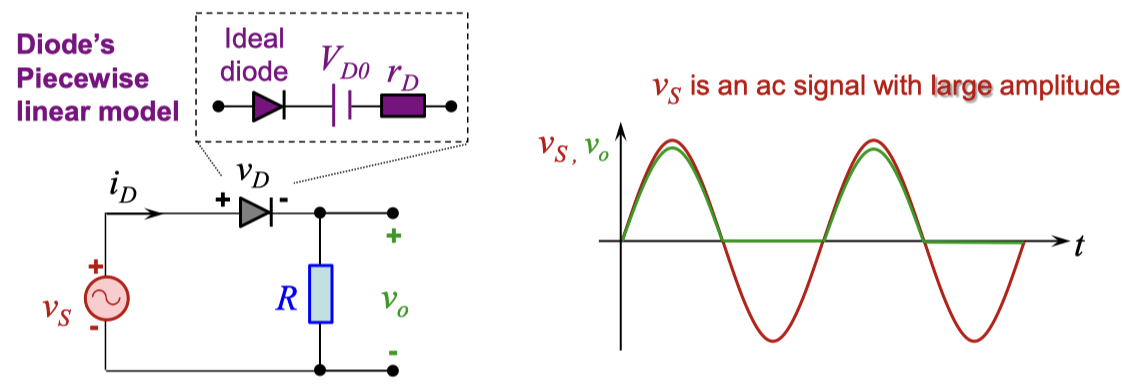
\includegraphics[width=1\linewidth]{image/halfrect.png}
    \end{figure} \\
    In the positive half, \(v_o = v_S -V_{D0}\) \\
    In the negative half, \(v_o = 0\) \\
    Full-wave Bridge rectifier\\
    \begin{figure}[h]
        \centering
        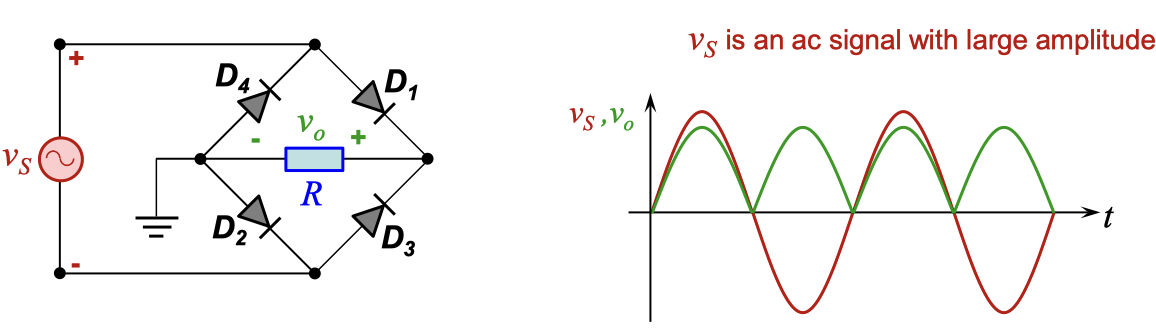
\includegraphics[width=1\linewidth]{image/fullwavebridge.png}
    \end{figure} \\
    Since there are two diodes involved, \(v_o = V_S - 2\times V_{D0}\) 
    \newpage
    Zener diode as voltage reference
    \begin{figure}[h]
        \centering
        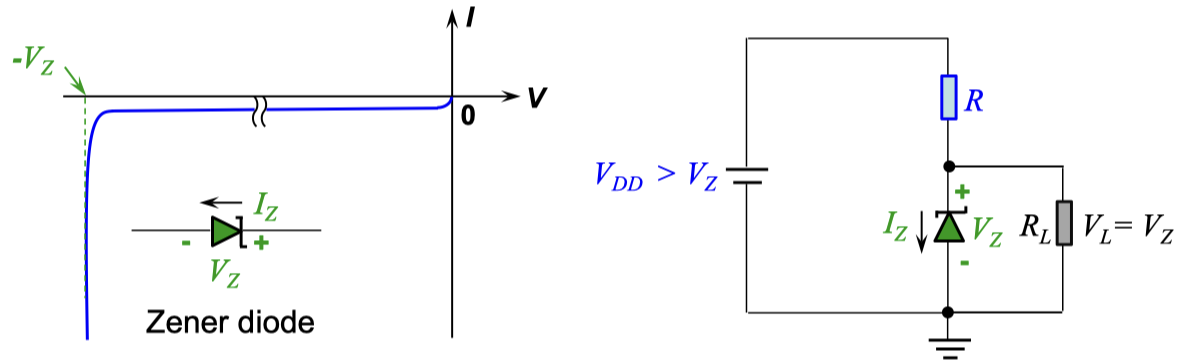
\includegraphics[width=1\linewidth]{image/zener.png}
    \end{figure}\\
    Since $V_Z$ is operating in the breakdown region, $R_L$'s voltage can be regulated by $V_Z$ as $V_L=V_Z$. Note that $I_Z \neq 0$.
    \item Charge stored and capacitance effect
    \begin{figure}[h]
        \centering
        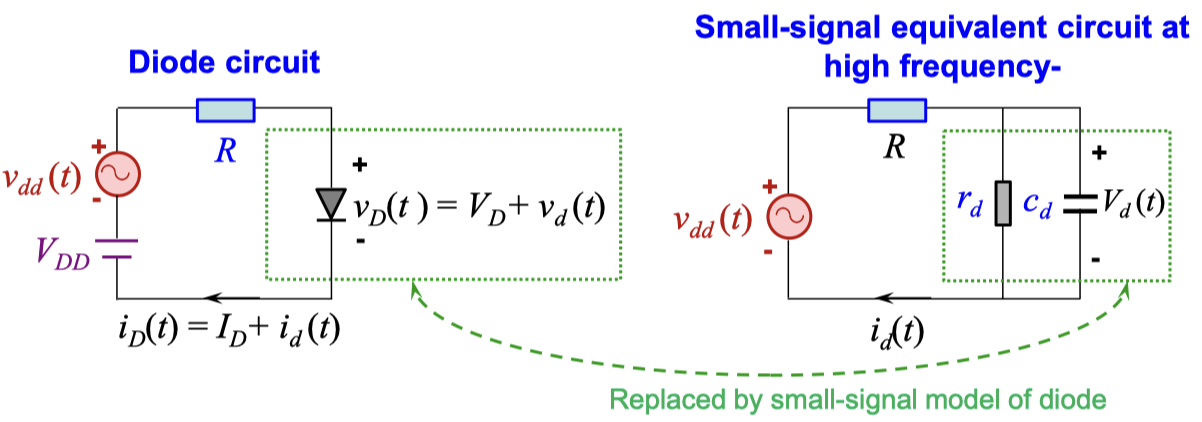
\includegraphics[width=1\linewidth]{image/diodesmall-signal.png}
    \end{figure}
\end{enumerate}
\subsubsection{Operational Amplifier}
\begin{enumerate}
    \item Opamp Schematic
    \begin{figure}[h]
        \centering
        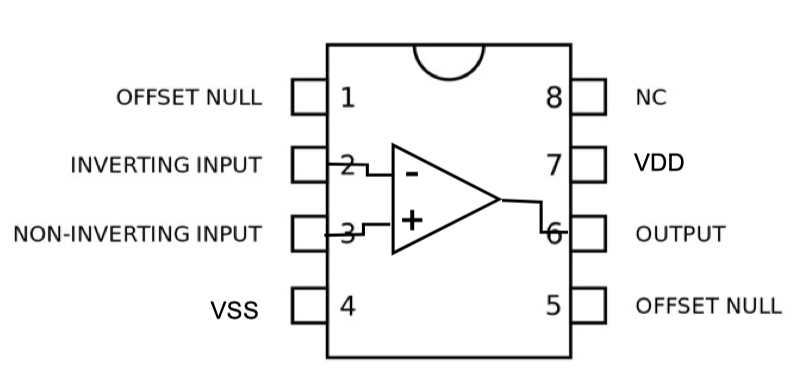
\includegraphics[width=0.5\linewidth]{image/opamp.png}
    \end{figure} \\
    For an ideal Opamp, $A = 10000 \rightarrow \infty$
    \item Inverting Amplifier\\
    \begin{circuitikz}
        \draw
        (0,0) node[op amp] (opamp) {}
        (opamp.+) node[left] {}
        (opamp.-) node[left] {}
        (opamp.out) node[right] {}
        (opamp.up) -- ++(0,0.5) node[vcc]{\(V_{CC}\)}
        (opamp.down) -- ++(0,-0.5) node[vee]{\(V_{EE}\)}
        
        % Inverting input
        (opamp.-) -- ++(-1.5,0) to[R, l_=\(R_{1}\), o-] ++(-2,0) node[left] {\(V_{in}\)}
        % Feedback resistor
        (opamp.-) ++(-1.5,0) -- ++(0,1.5) to[R, l=\(R_2\)] ++(3,0) -| (opamp.out)
        % Output
        (opamp.out) -- ++(1,0) node[right] {\(V_{out}\)}
        % Ground
        (opamp.+) -- ++(0,-0.5) node[ground] {};
    \end{circuitikz} \\
    The transfer function for inverting Amplifier is 
    \begin{equation}
        \frac{v_{out}}{v_{in}} = -\frac{R_2}{R_1}
    \end{equation}
    Proof: \\
    \(v_1 = v_{\_} \approx v_{+} = 0\) [Virtually short to ground] \\
    \(\displaystyle \frac{v_{in}-v_1}{R_1} = \frac{v_1 - v_{out}}{R_2}\)\\
    \(\displaystyle \frac{v_{in}}{R_1} = \frac{-v_{out}}{R_2}\) \\
    \(\displaystyle \frac{v_{out}}{v_{in}} = -\frac{R_2}{R_1}\)
    \item Non-Inverting Amplifier
    \begin{center}
        \begin{figure}[h]
            \centering
            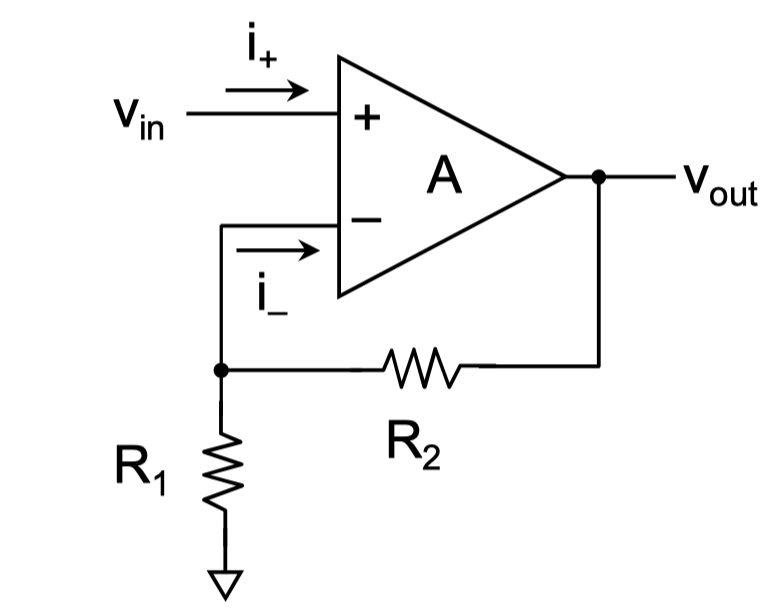
\includegraphics[width=0.4\linewidth]{image/noninopamp.png}
        \end{figure}
    \end{center}
    The transfer function for Non-Inverting Amplifier is 
    \begin{equation}
        \frac{v_{out}}{v_{in}} = (1+\frac{R_2}{R_1})
    \end{equation}
    Proof: \\
    $\displaystyle v_{\_} \approx v_{+} = v_{in}$ [Virtually short to ground] \\
    $\displaystyle v_{\_} = v_{out} \times \frac{R_1}{R_1 + R_2} = v_{in}$ [$i_{+} = i_{\_} = 0$]
    $\displaystyle \frac{v_{out}}{v_{in}} = (1+\frac{R_2}{R_1})$
\end{enumerate}


\newpage
\subsection{Microelectronics Materials and Devices}
\subsubsection{Crystal Structure}
\begin{enumerate}
    \item Type of solids: \\
    Solids are ordered according to 3 types: amorphous, polycrystalline, and single crystal.
    \begin{figure}[h]
        \centering
        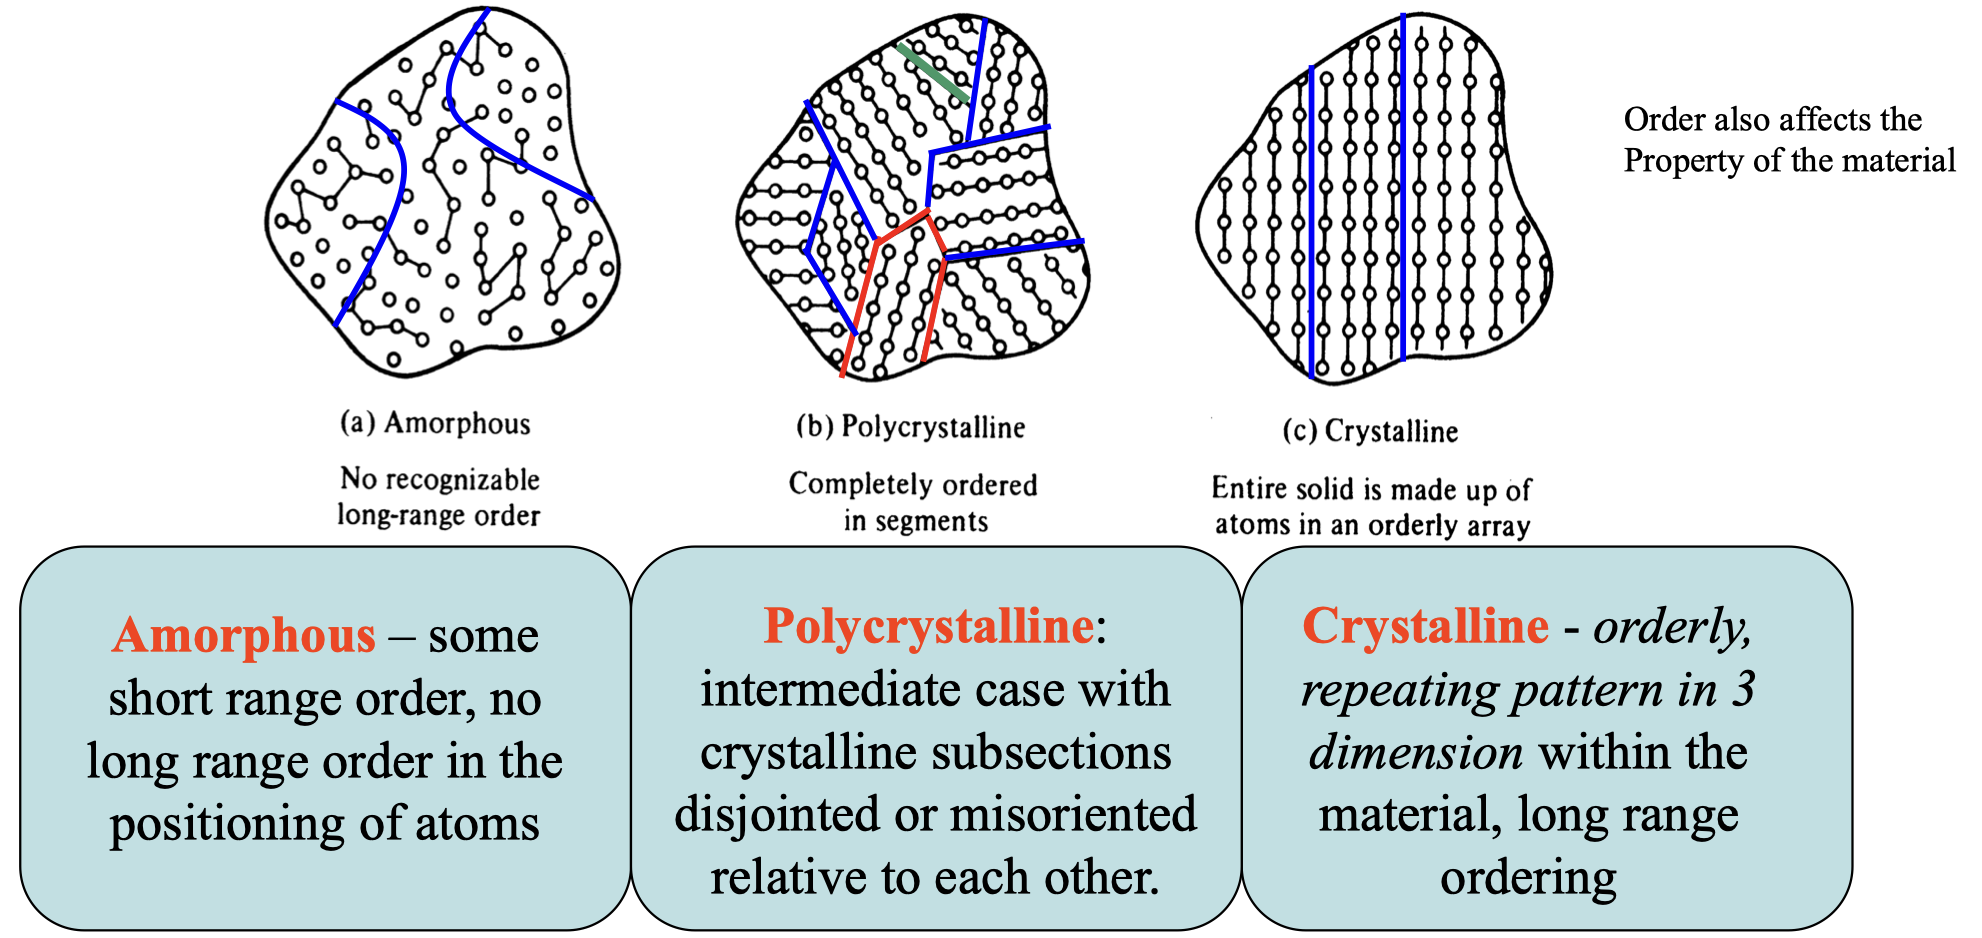
\includegraphics[width=0.75\linewidth]{image/crstal.png}
    \end{figure}
    \item How to describe a crystal structure\\
    Crystal Structure = Lattice Point + Basis \\
    Basis = single atom OR group of atoms attached to each lattice point \\
    \begin{figure}[h]
        \centering
        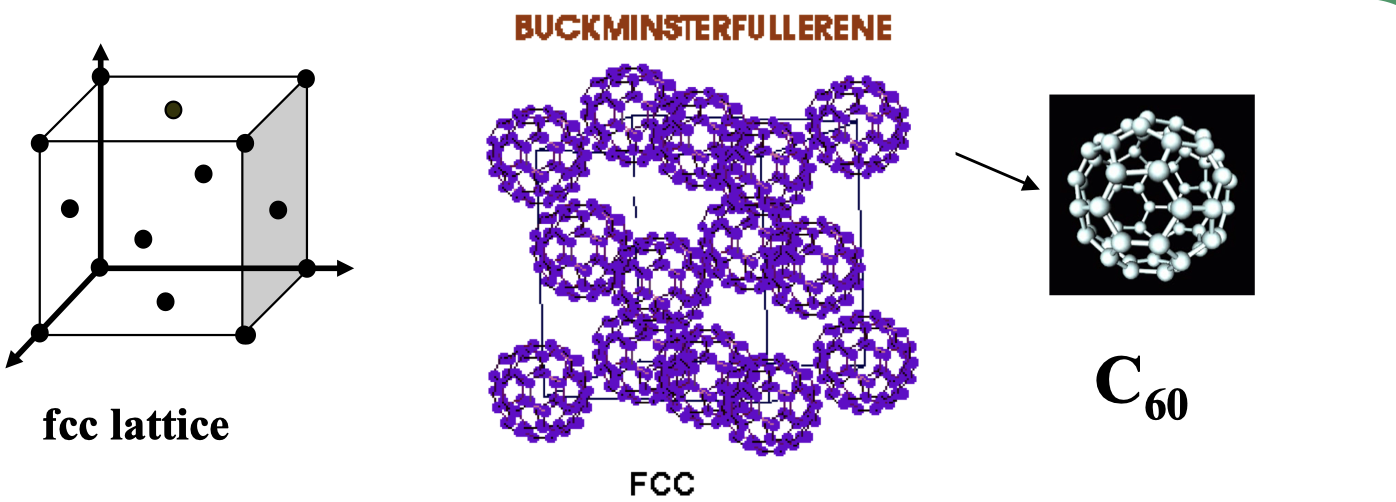
\includegraphics[width=0.8\linewidth]{image/latticestructure.png}
    \end{figure}
    \item Unit Cell \\
    Unit Cell = small portion of any given crystal that can be used to reproduce the crystal. \\
    Lattice angles: the inter-axial angles $\alpha$, $\beta$ and $\gamma$. \\
    Lattice constants: all of the parameters of the unit cell. \\
    Volume: $\displaystyle V = |\Vec{a}\cdot\Vec{b}\times\Vec{c}|$
    \begin{figure}[h]
        \centering
        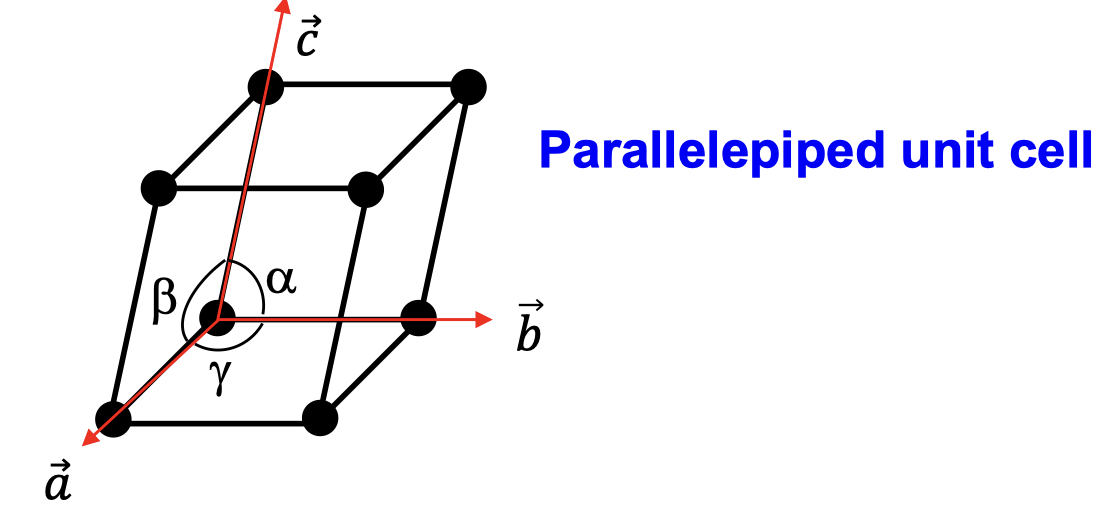
\includegraphics[width=0.75\linewidth]{image/unicell.png}
    \end{figure}
    \item 3D Bravais Lattice Types
    There are only 14 \textbf{unique} Bravais Lattices (unit cells) to fill space with a periodic arrangement of points. \\
    The ones we are interested are: bcc, fcc and hcp.
    \begin{figure}[h]
        \centering
        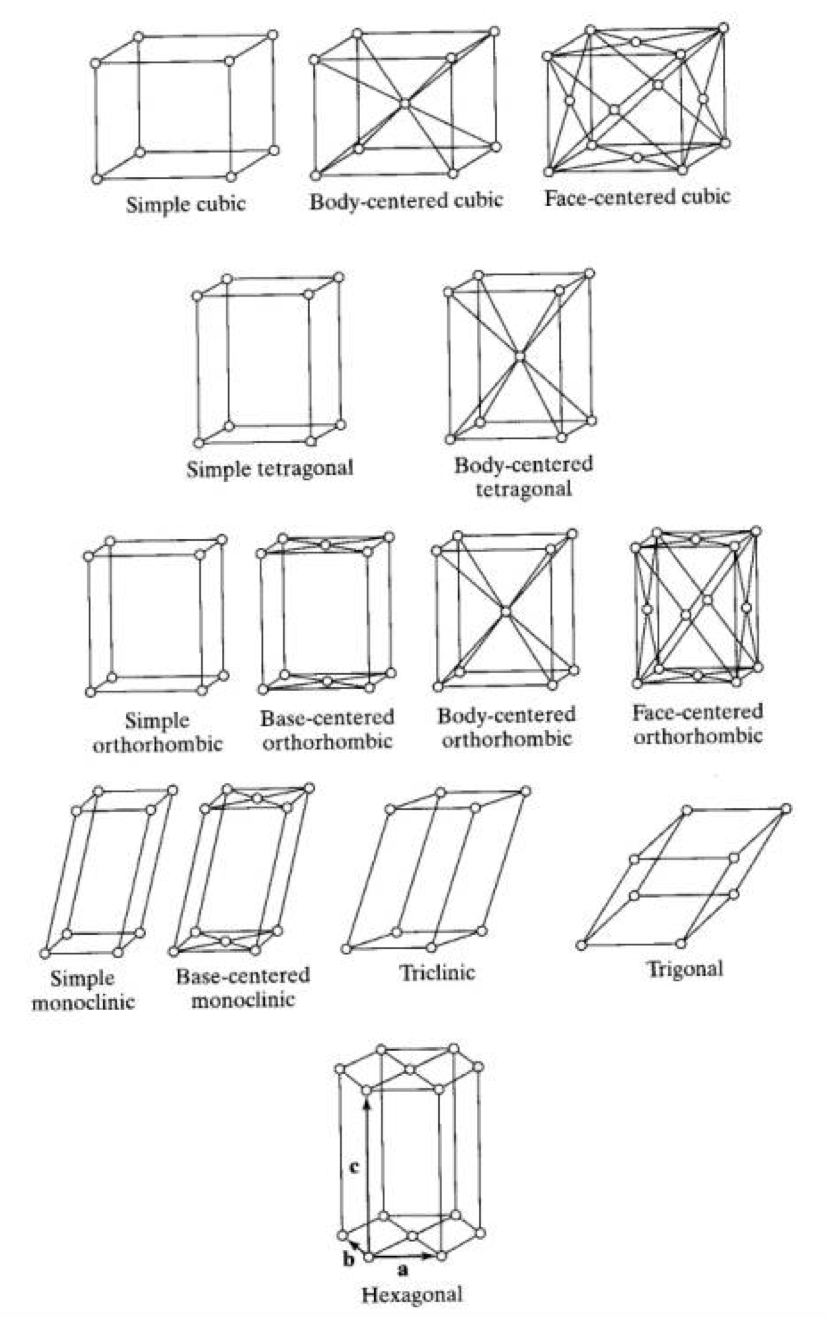
\includegraphics[width=0.5\linewidth]{image/14cellls.png}
    \end{figure}
    \item Cubic Lattices\\
    \begin{figure}[h]
        \centering
        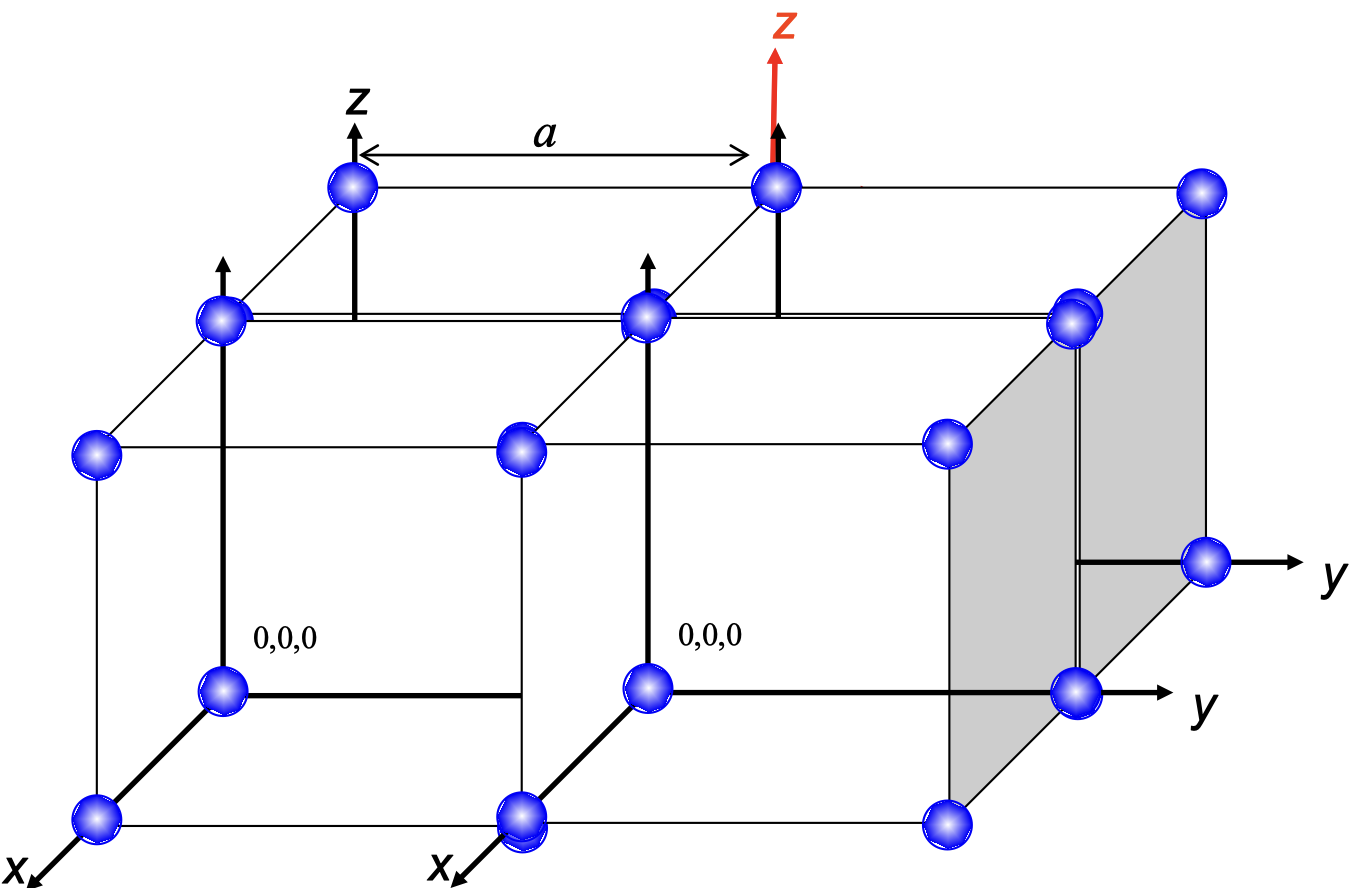
\includegraphics[width=0.75\linewidth]{image/cubiclattic.png}
    \end{figure}
    Cubic lattices can be specified by a single lattice constant \textcolor{red}{a}. \\
    Note: Since each atom is shared by 8 unit cells, only 1/8 of each corner atom is inside each unit cell. \\
    Example of SC Metals : \ce{Po}
    \item Body-centred Cubic (Bcc) Structure
    \begin{figure}[h]
        \centering
        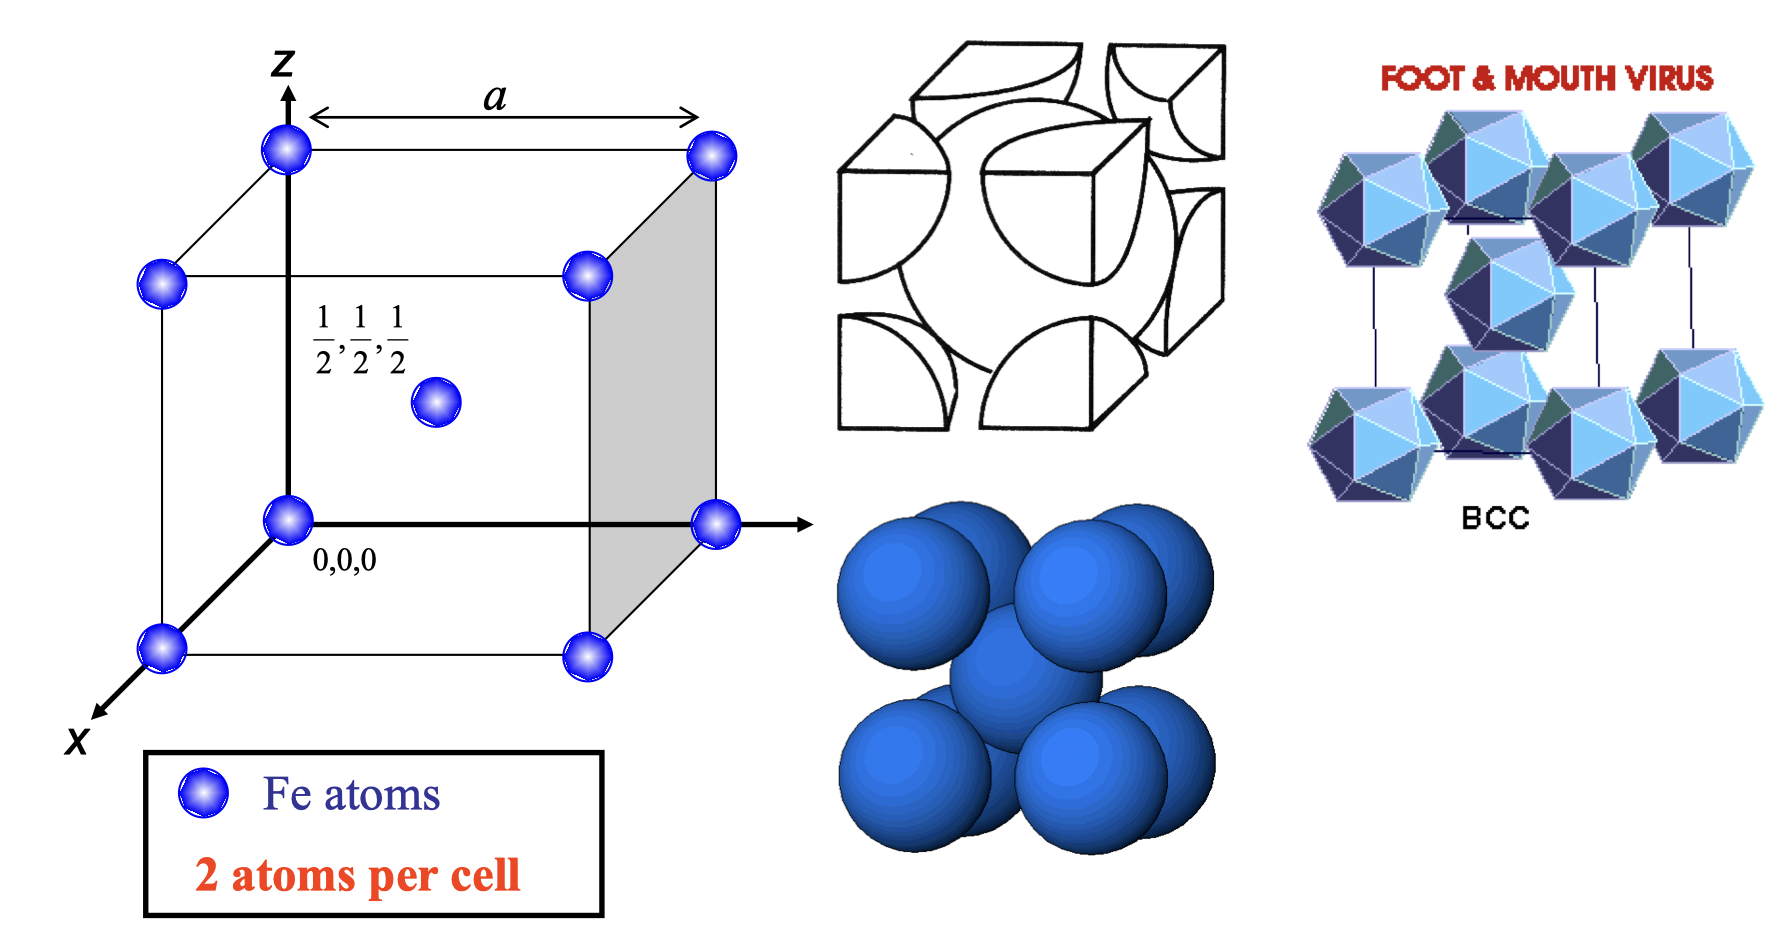
\includegraphics[width=0.75\linewidth]{image/bcc.png}
    \end{figure} \\
    Example of Bcc Metals: \ce{Fe}, \ce{W}, \ce{Mo}, \ce{Nb}, \ce{Ta}, \ce{V}, \ce{Cr}
    \newpage
    \item Face-centered Cubic (Fcc) Structure 
    \begin{figure}[h]
        \centering
        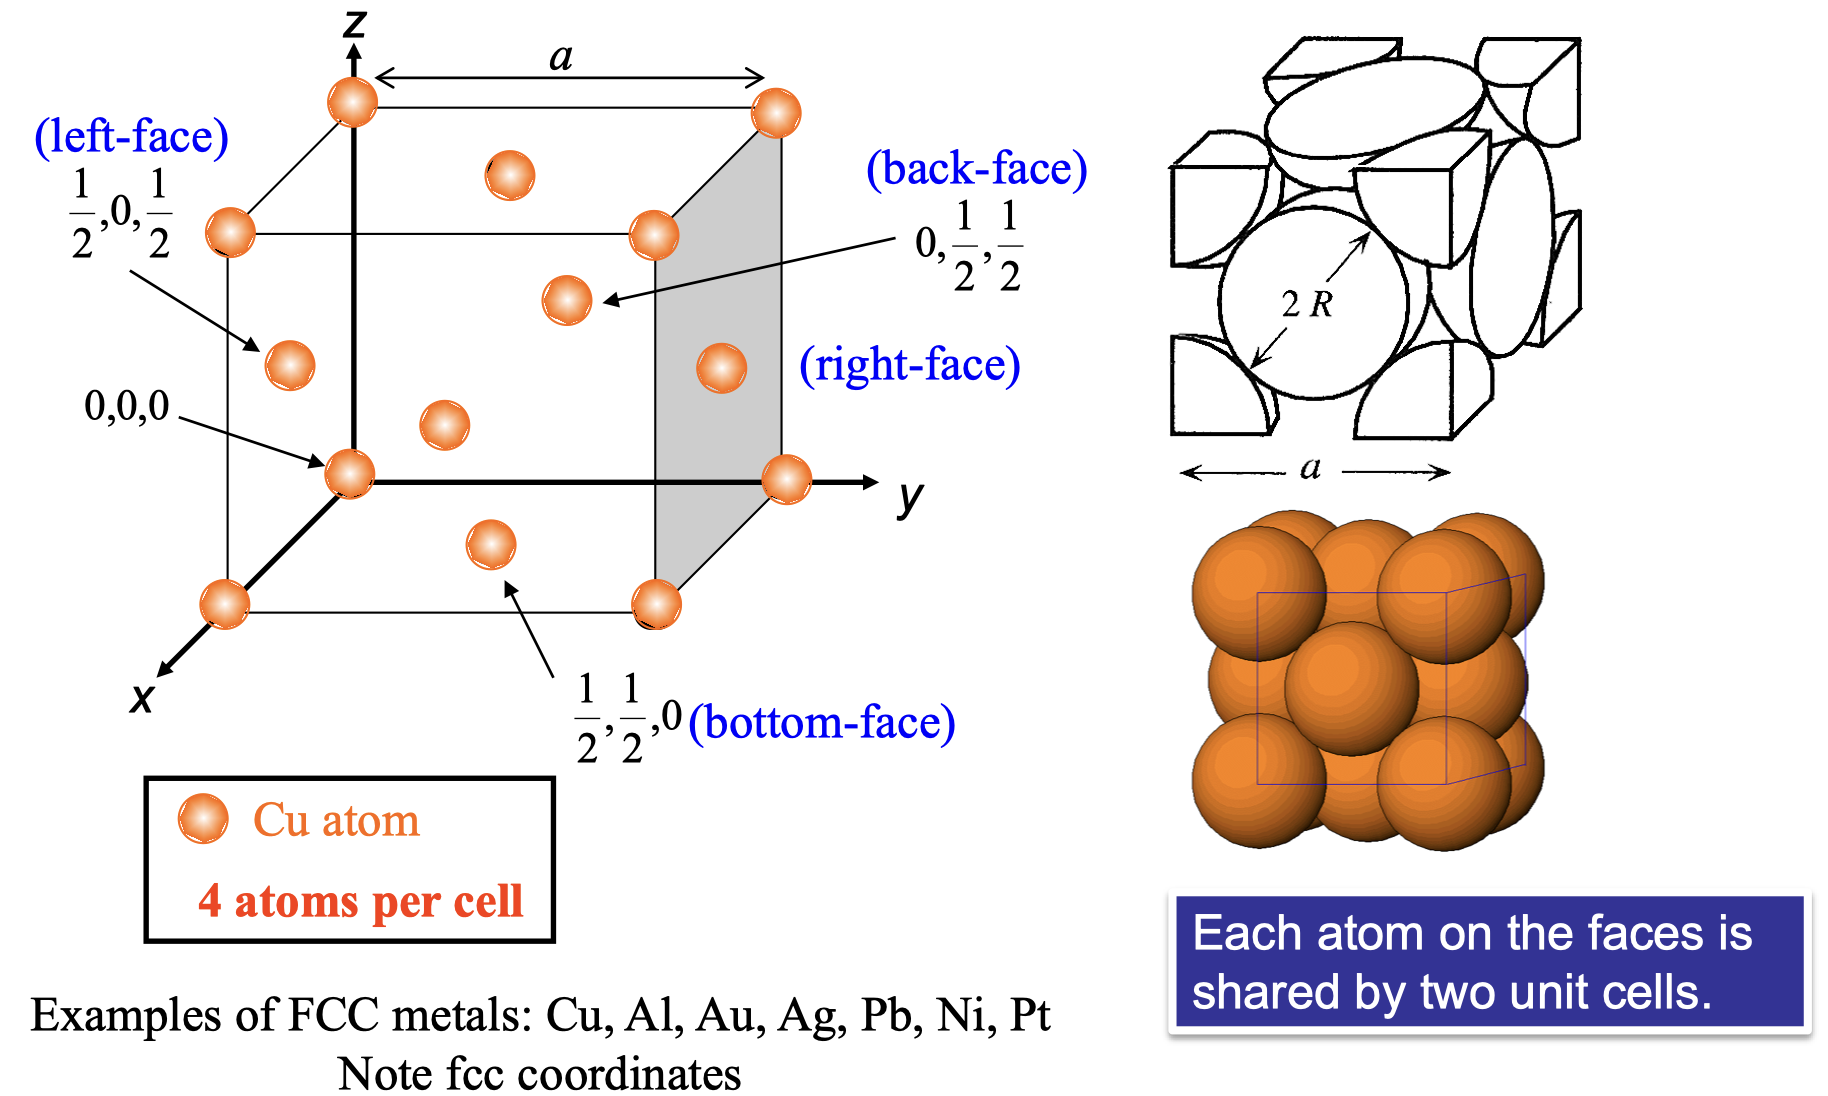
\includegraphics[width=0.75\linewidth]{image/fcc.png}
    \end{figure}
    \item Fcc Derivatives (Diamond Structure) 
    \begin{figure}[h]
        \centering
        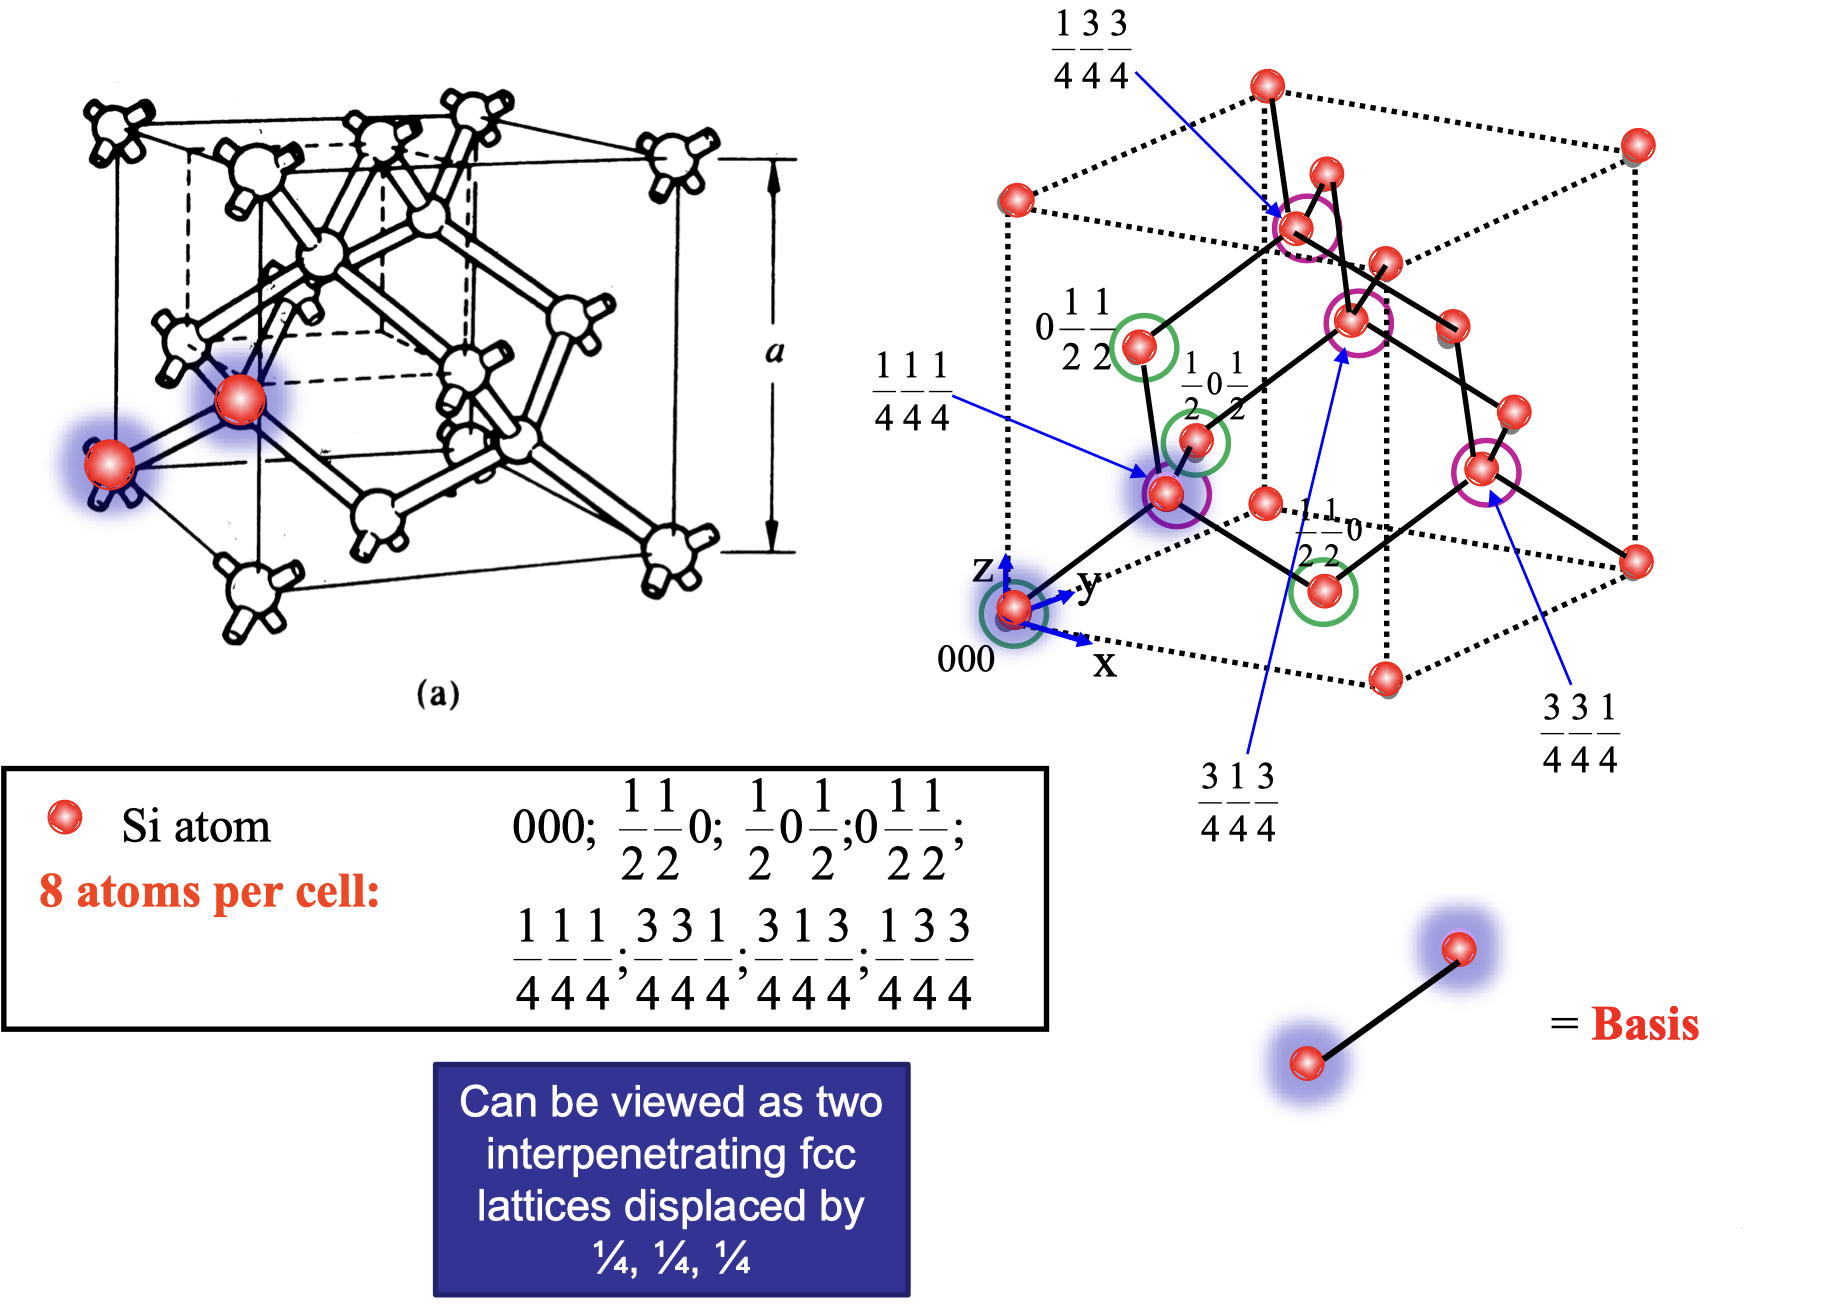
\includegraphics[width=0.75\linewidth]{image/diamondsturc.png}
    \end{figure} 
    \newpage
    \item Fcc Derivatives (Zinc-Blende Structure) 
    \begin{figure}[h]
        \centering
        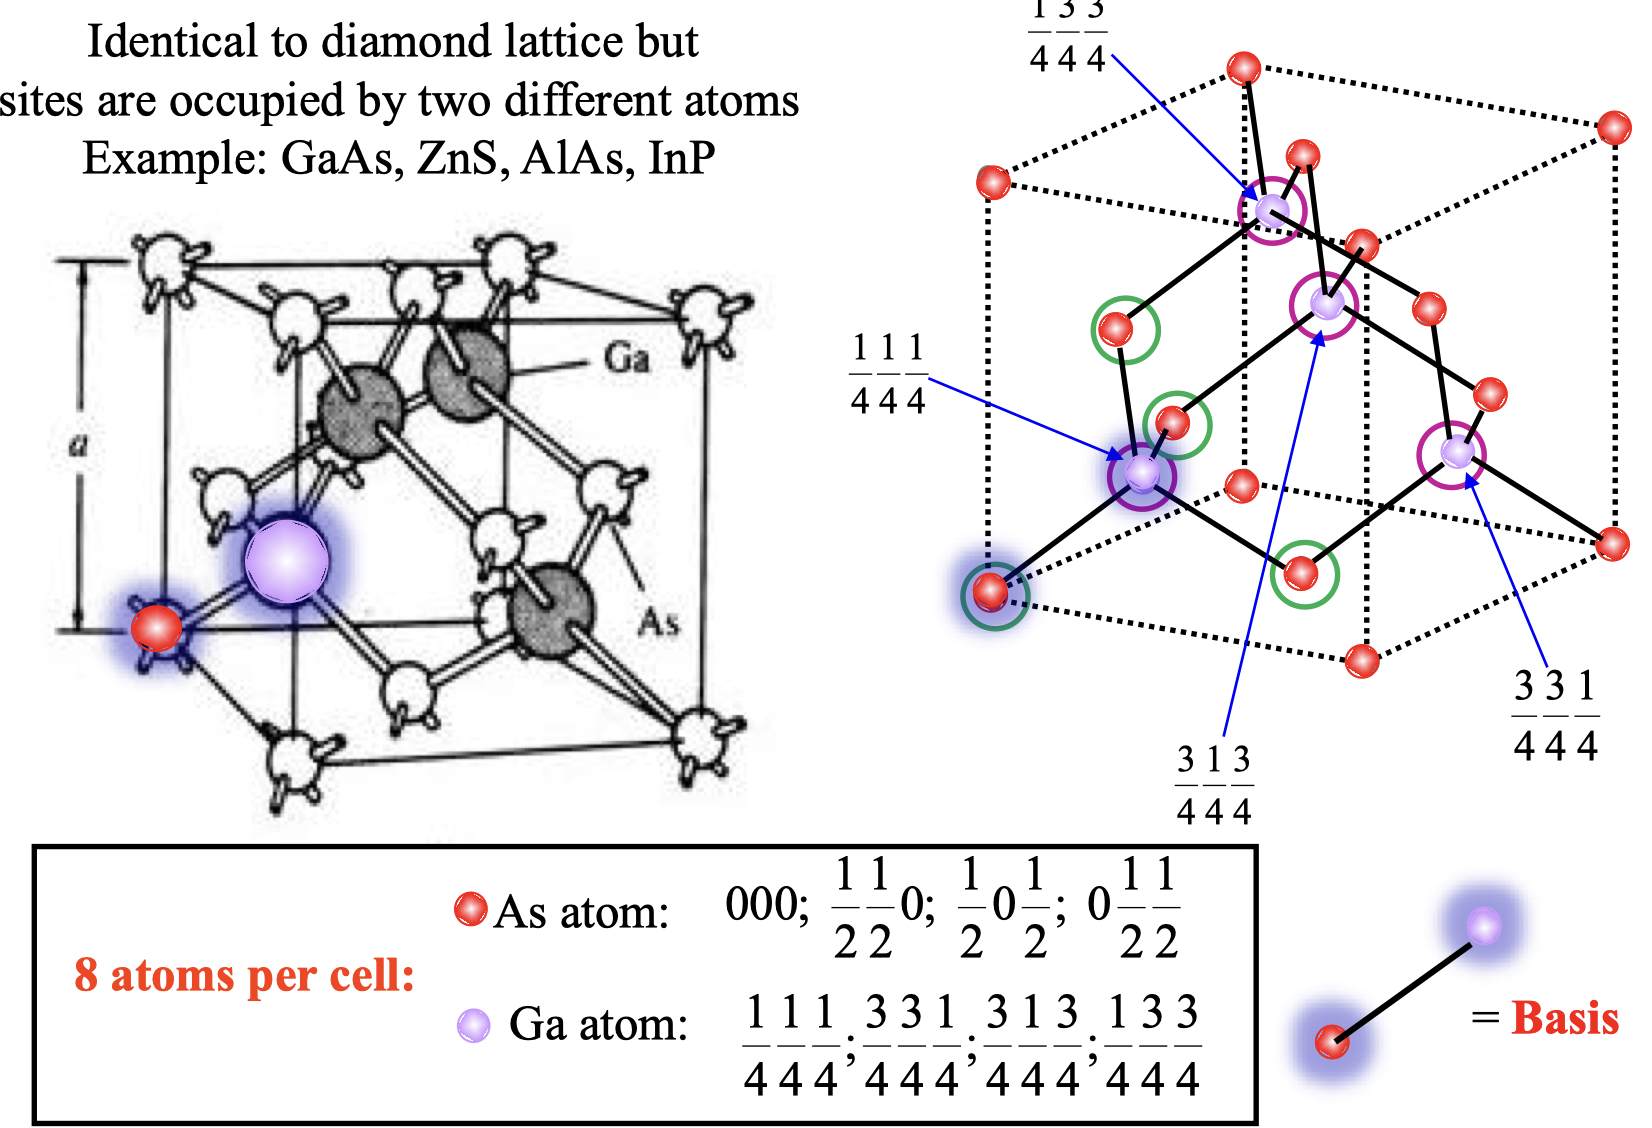
\includegraphics[width=0.75\linewidth]{image/zincblende.png}
    \end{figure}
    \item Sodium Chloride (Rocksalt) structure
    \begin{figure}[h]
        \centering
        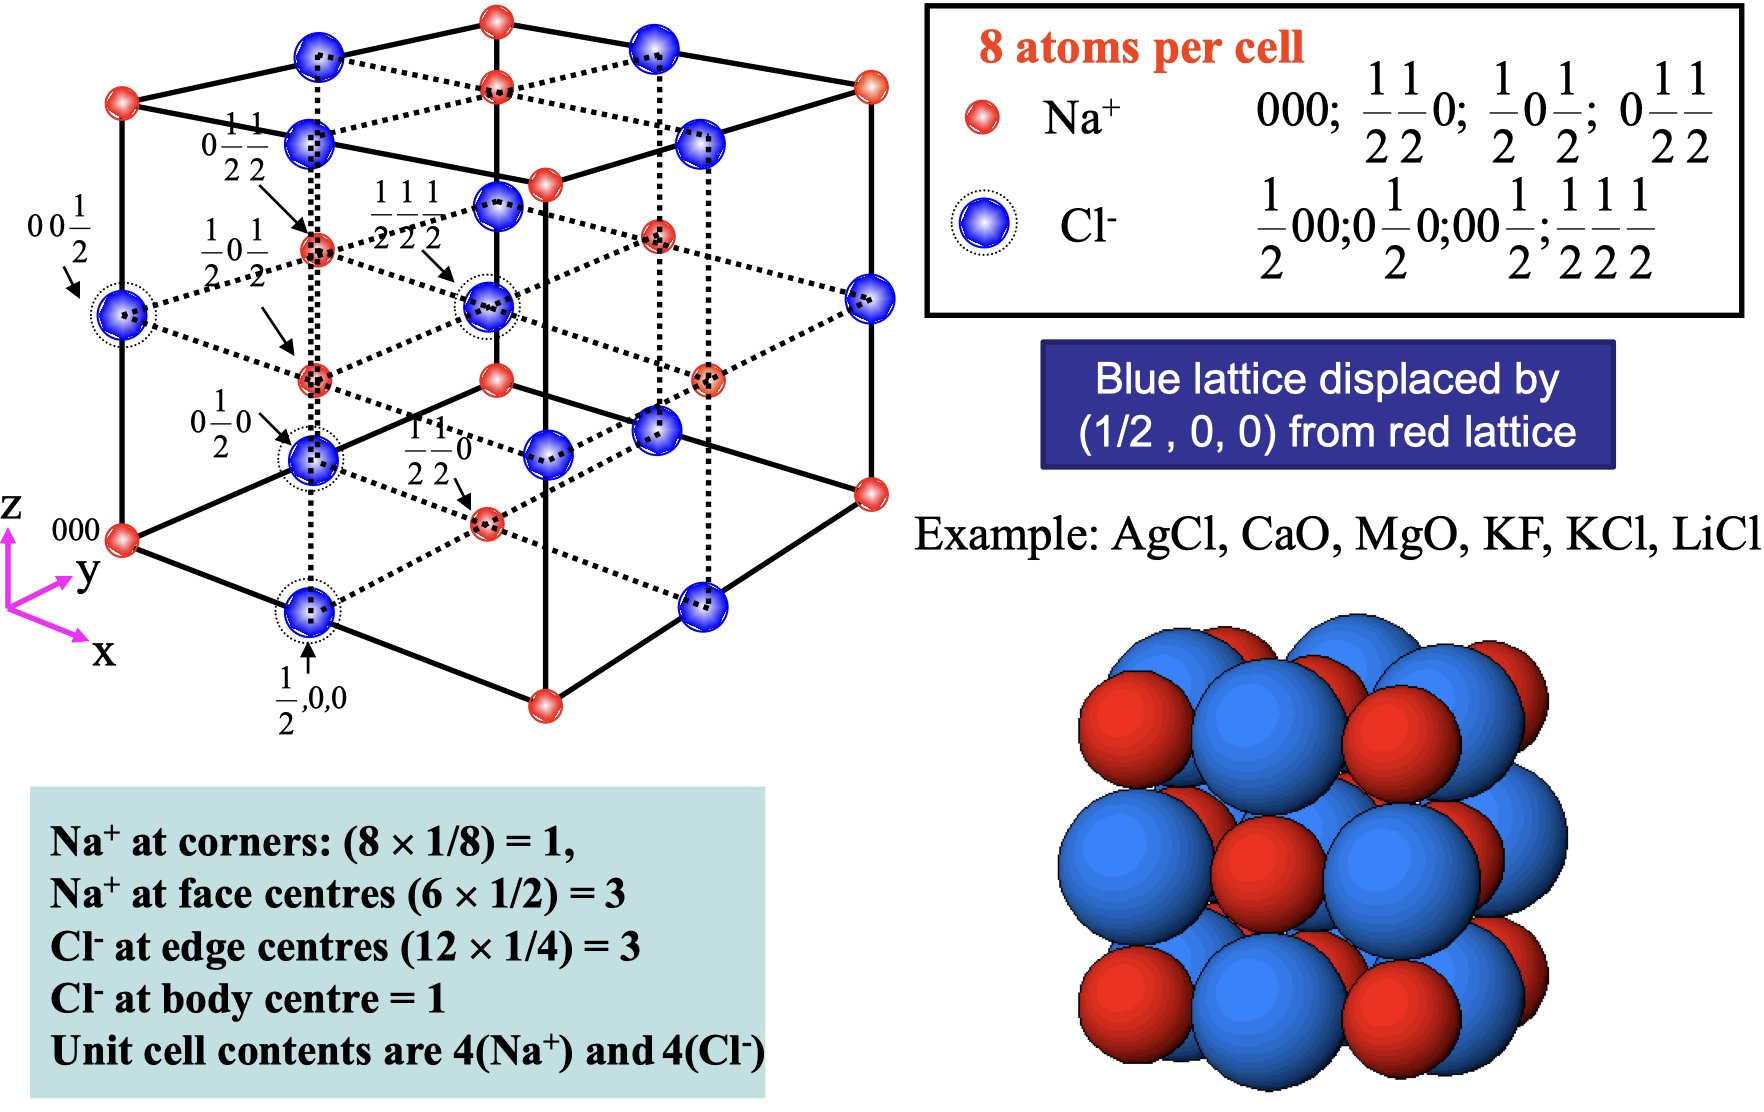
\includegraphics[width=0.75\linewidth]{image/rockcet.png}
    \end{figure}
    \newpage
    \item Hexagon lattice \\
    In 2D, close packed layers is the most efficient way of packing equal sized spheres. They can be stacked to closely packed to give 3D structure.
    \begin{figure}[h]
        \centering
        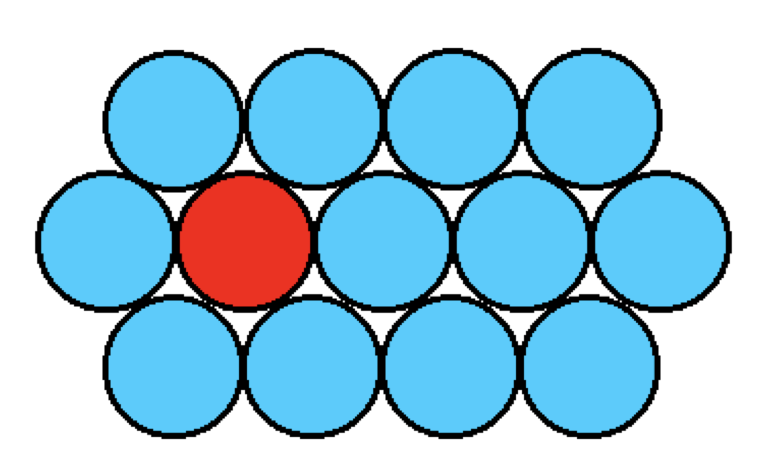
\includegraphics[width=0.5\linewidth]{image/2dgraph.png}
    \end{figure} \\
    It can have A position sequence $\ldots ABABABAB\ldots$ and this is  Hexagonal close packing (hcp). \\ 
    It can also position sequence $\ldots ABCABCABCABC\ldots$ and this is  Cubic close packing (ccp). \\
    The difference between hcp and ccp
    \begin{figure}[h]
        \centering
        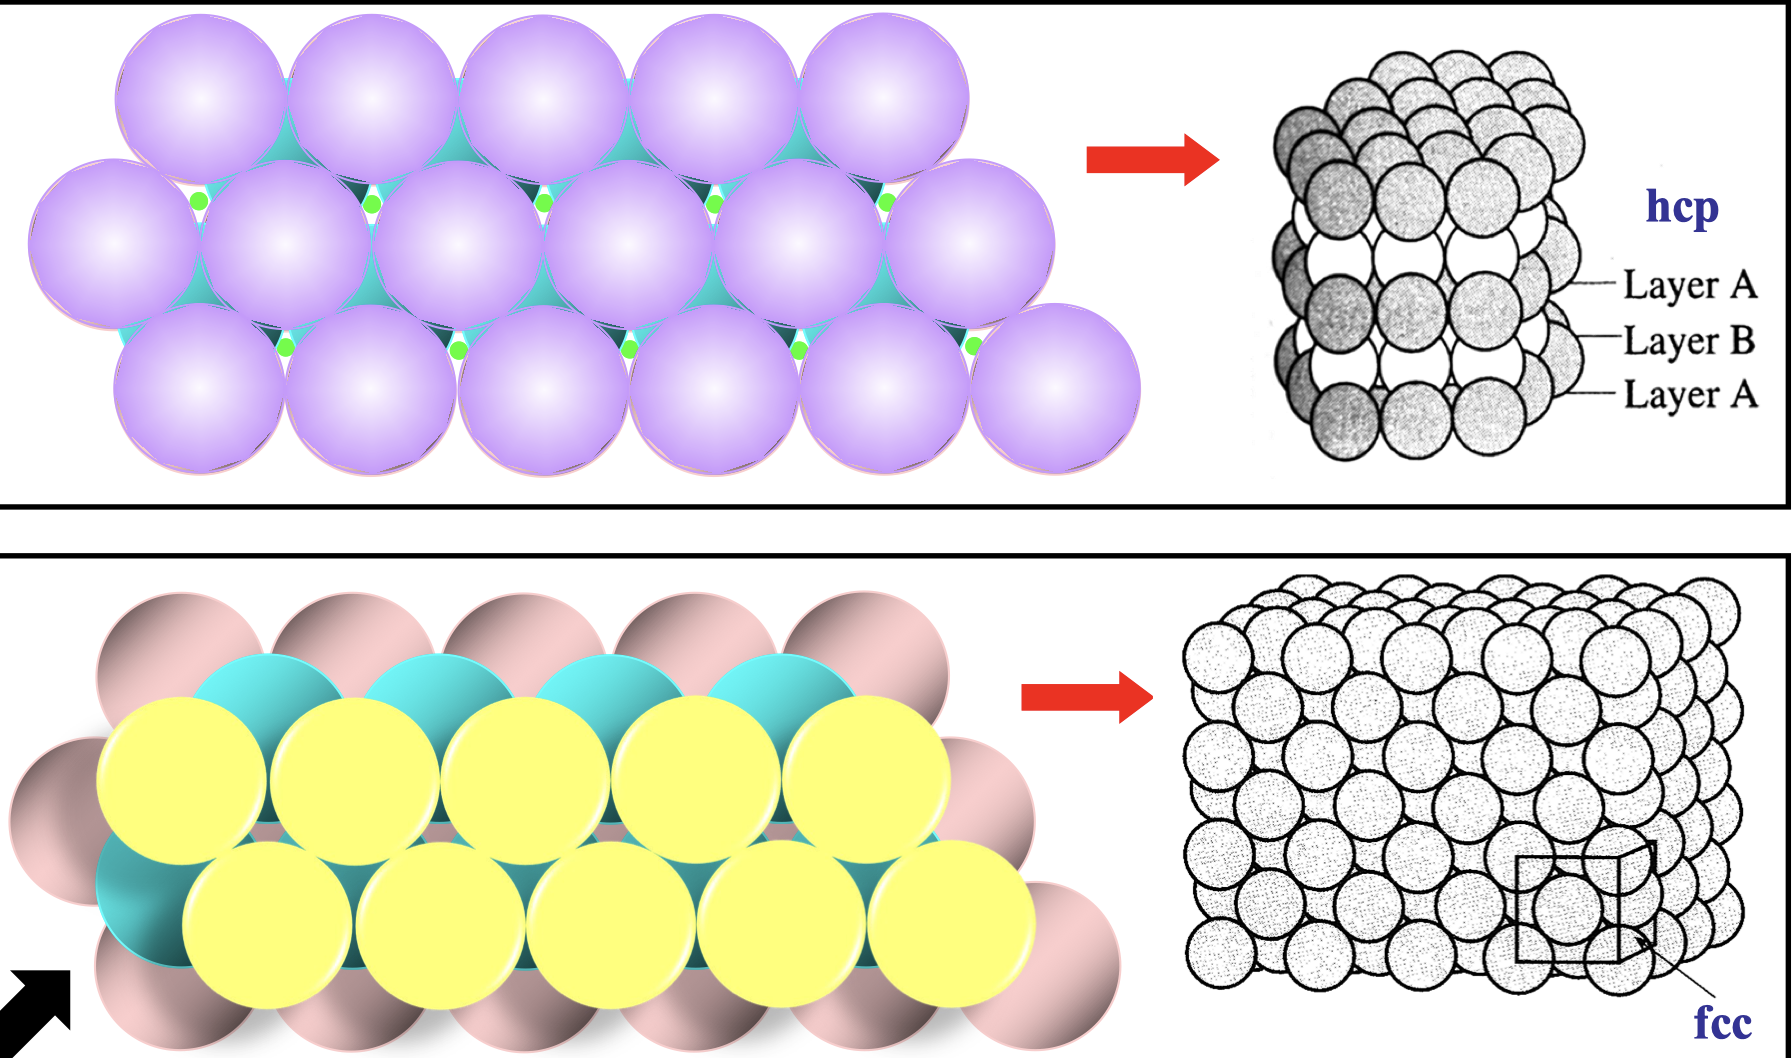
\includegraphics[width=0.75\linewidth]{image/hcpccp.png}
    \end{figure}
    \item Hexagonal System (Number of atoms)
    \begin{figure}[h]
        \centering
        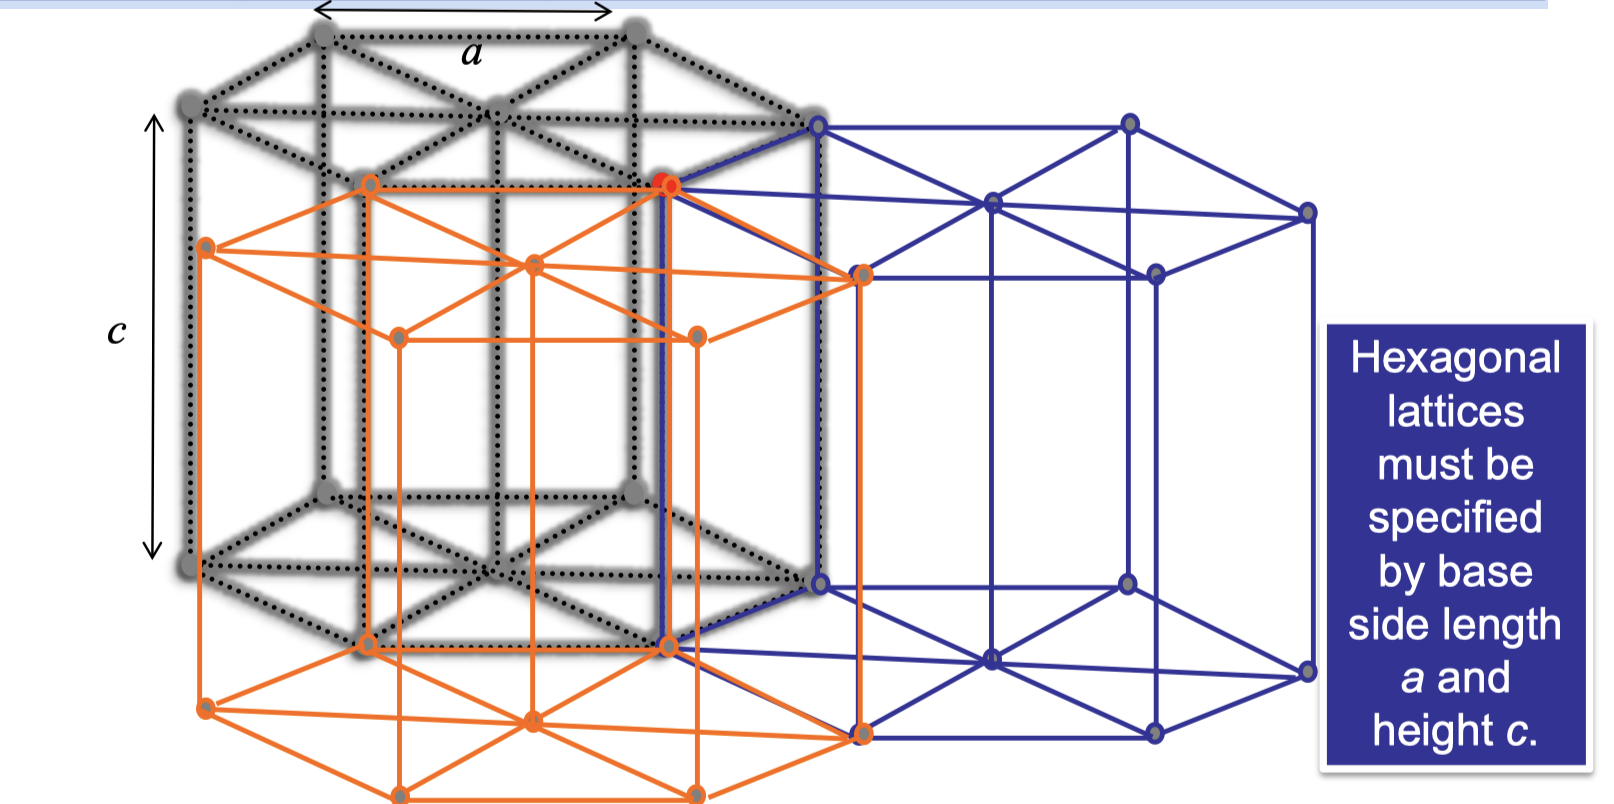
\includegraphics[width=0.5\linewidth]{image/hcpno.png}
    \end{figure} \\
    Number of atoms per unit cell = 3.\\
    Each corner atom shared with 6 neighbour cells. Total 12 neighbour gives 2 atoms. $\frac{1}{6} \times 12 = 6$\\
    The centered atom at the top and bottom of the cell shared half with neighboring cell. $\frac{1}{2} \times 2 = 1$ \\
    In total: $2+1 = 3$.
    \item Atomic Packing Factor \\
    Maximum fraction of the volume in a unit cell occupied by the atoms.\\
    Assume that the atoms are closely packed and that they can be treated as hard spheres. This fraction is called atomic packing factor (APF) or packing density.
    \[APF = \frac{\text{Number of atoms per cell $\times$ volume of one atom}}{\text{volume of unit cell}}\]
    \vspace{1cm}
    \begin{minipage}{0.5\textwidth}
        Number of atoms: 4 \\
        Volume of each atoms: $\displaystyle \frac{4}{3}\pi R^3$ \\
        Unit cell Volume : $\displaystyle a^3 = (2\sqrt{2}R)^3$ \\
        $\displaystyle APF = \frac{\frac{4}{3} \pi R^3}{(2\sqrt{2}R)^3} = 0.74$
    \end{minipage}
    \begin{minipage}{0.5\textwidth}
        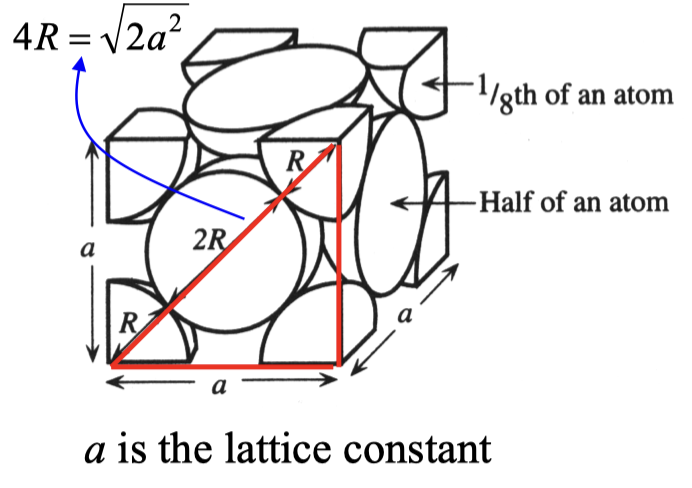
\includegraphics[width=0.75\linewidth]{image/atomcellvol.png}
    \end{minipage}
    \item Atomic Packing factor for different structures
    \begin{center}
    \begin{tabular}{|l|c|c|c|c|}
    \hline
        \textbf{Structure} & \textbf{Radius} & \textbf{Atom/unit cell} & \textbf{APF} & \textbf{Coordination no.}\\ \hline
        Simple cubic       & $\frac{a}{2}$   & 1                       & $\frac{\pi}{6} = 52\%$ & 6\\ \hline
        BCC                & $\frac{\sqrt{3}a}{4}$ & 2                 & $\frac{\pi\sqrt{3}}{8} = 68\%$ & 8\\ \hline
        FCC                & $\frac{\sqrt{2}a}{4}$ & 4                 & $\frac{\pi\sqrt{2}}{6} = 74\%$ & 12\\ \hline
        Diamond            & $\frac{\sqrt{3}a}{8}$ & 8                 & $\frac{\pi\sqrt{3}}{16} = 34\%$ & \\ \hline
    \end{tabular}
    \end{center}
    \item Miller Indices for Crystal Planes\\
    Steps to write \textit{hkl} plane notations
    \begin{enumerate}
        \item Find the plane intercepts.
        \item Take the reciprocals.
        \item Find the smallest three integers having the same ratio.
        \item Write down the indices of the plane. E.g. (233) -- (\textit{hkl})
    \end{enumerate}
    Take note that a group of equivalent planes is denoted by braces around the indices. For example, $(100),(010),(001),(\bar{1}00),(0\bar{1}0),(00\bar{1})$ are collectively denoted as $\{100\}$.
    \item Distance between adjacent (\textit{hkl}) planes.\\
    \begin{equation}
        d_{hkl} = \frac{a}{\sqrt{h^2+k^2+l^2}}
    \end{equation}
    $d$ is the distance from a selected origion containing one plane and another parallel plane with the same indices which is closest to it.
    \item Directions in Crystal \\
    Family of directions can be represented by : $<100>$
    \item Crystal-direction vector \\
    For a cubic crystal, the angle $\theta$ between directions $[h_1k_1l_1]$ and $[h_2k_2l_2]$ is given by
    \begin{equation}
        \cos \theta = \frac{h_1h_2+k_1k_2+l_1l_2}{\sqrt{(h_1^2+k_1^2+l_1^2)(h_2^2+k_2^2+l_2^2)}}
    \end{equation}
    An typical application of Miller indices is Crystal Plane and Crystal Directions.
    \item Atomic Concentration 
    \[\text{Atomic concentration} = \frac{\text{Number of atoms}}{\text{unit volume}}\]
    \item Volume Density 
    \begin{align*}
        \rho_\nu &= \frac{\text{Mass of all atoms in the unit cell}}{\text{volume of the unit cell}} \\
        &= \text{Atomic concentration} \times \text{mass}
    \end{align*}
    \item Planar concentration 
    \[\text{Planar concentration} = \frac{\text{no. of atoms who centers are intersected by area }}{\text{area}}\]
    \newpage
    \item X-ray and diffraction grating \\
    Bragg's Law
    \begin{equation}
        2d_{hkl}\sin \theta= n\lambda
    \end{equation}
    \begin{figure}[h]
        \centering
        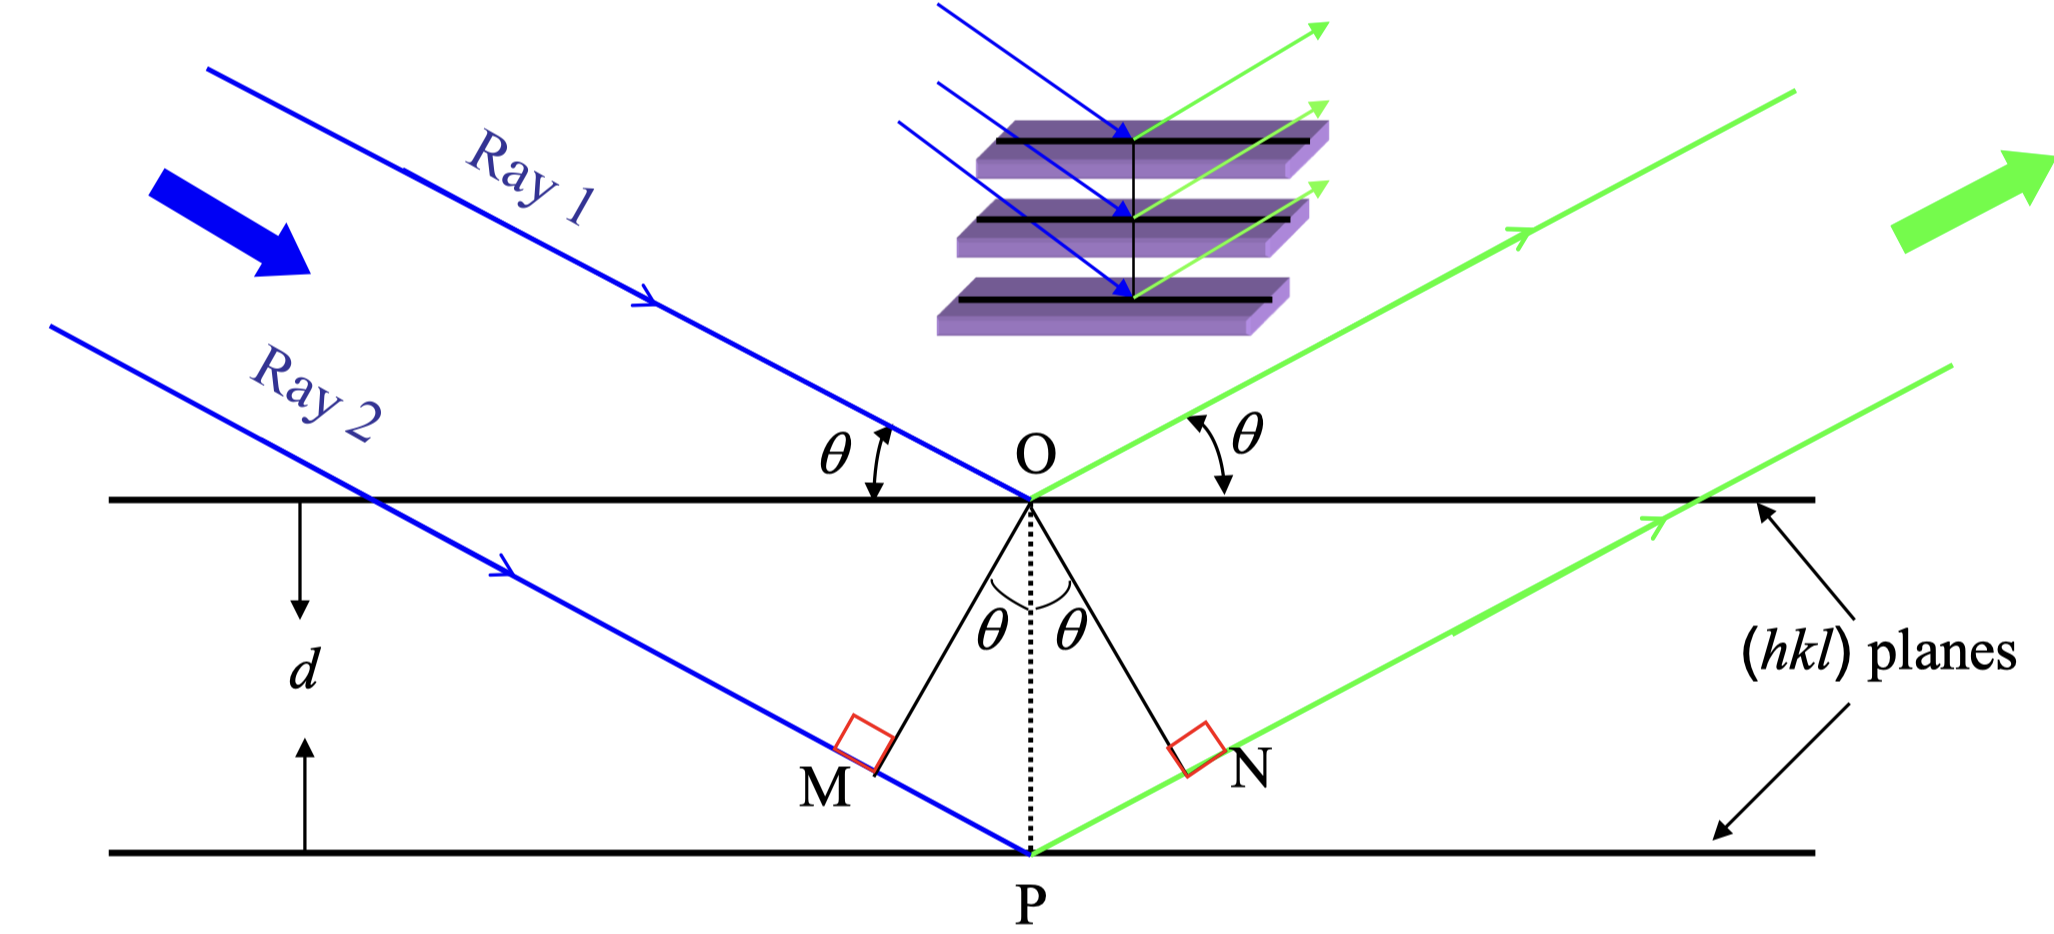
\includegraphics[width=0.75\linewidth]{image/bragglaw.png}
    \end{figure}
    For constructive interference $\displaystyle n\lambda = MP + PN$ \\
    Take note that  the higher the planar concentration (or planar density) in a crystalline material, the higher the intensity of the peak in an X-ray diffraction (XRD).
    
\end{enumerate}
\subsubsection{Band Theory}
\begin{enumerate}
    \item Bohr Atomic Model \\
    The voltage due to charge at radius $r$ is 
    \[V(r) = \frac{+e}{4\pi \varepsilon_0 r}\]
    Potential Energy is
    \[E_{PE}(r) = Q\cdot V = \frac{-e^2}{4\pi \varepsilon_0 r}\]
    Take note that $\varepsilon_0 = 8.85\times 10^{-12} F/m$ \\
    Kinetic energy of the orbiting electron is 
    \[E_{KE}(r) = \frac{e^2}{8\pi \varepsilon_0 r}\]
    Total energy is 
    \[E_{tot}(r) = E_{PE}+E_{KE} = \frac{-e^2}{8\pi \varepsilon_0 r}\]
    According to Bohr atomic model, electrons can only exist at fixed radii given by 
    \begin{equation}
        r_n = n^2 \hbar^2 \frac{4\pi \varepsilon_0}{m_0 e^2}\; :\; n = 1,2,3\ldots 
    \end{equation}
    Where $m_0 = 9.108\times 10^{-31} kg$ and $\hbar = \frac{h}{2\pi}$, $h = 6.625\times 10^{-34} J.s$
    \item Electronic Configuration \\
    \begin{figure}[h]
        \centering
        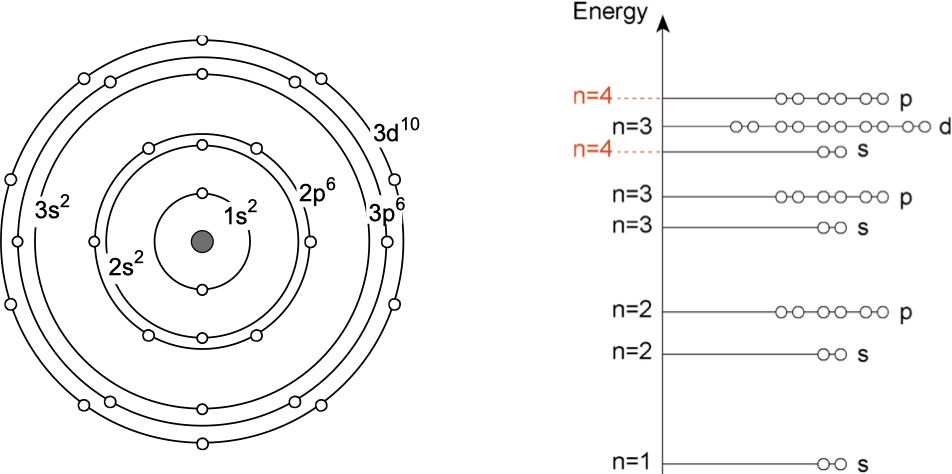
\includegraphics[width=0.75\linewidth]{image/eleconifg.png}
    \end{figure}
     \\
    \item Band Theory-Energy Levels in Atoms \\
    Split in energy level when shells overlap. \\
    The degree of split depends on the extent of the overlap. \\
    Electrons will fill up the lowest possible energy states. \\
      \\
    \begin{minipage}{0.5\textwidth}
        For a large number of atoms, a band of very closely-spaced discrete energy levels is formed from each atomic energy level. \\
        The separation between energy levels is very small. Hence the values of energy an electron can have within a band is quasi-continuous.
    \end{minipage}
    \begin{minipage}{0.4\textwidth}
        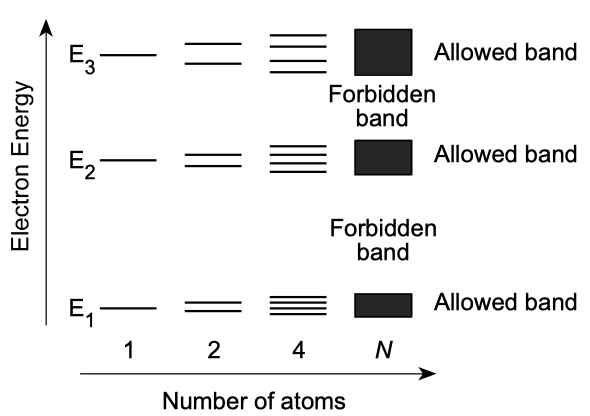
\includegraphics[width=1\linewidth]{image/energybandd.png}
    \end{minipage} 
    \item Forbidden and Allowed bands\\
    Depending on the way in which the electron shells interact, some bands can overlap each other, forming a continuous band of energies without any breaks. \\
    If The energy bands are separated, then we end up with forbidden bands between allowed bands.
    \begin{figure}[h]
        \centering
        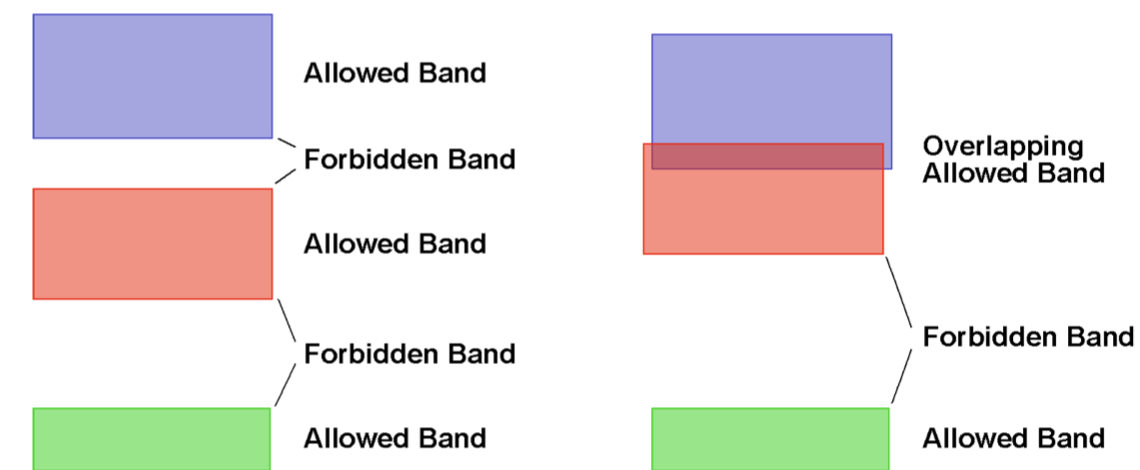
\includegraphics[width=0.75\linewidth]{image/forbidden.png}
    \end{figure}
    When the bands are formed beyond the vacuum level, electrons are free and can take on any energy value.
    \item Electrical Conduction \\
    For the energy to conduct electricity, it has to be a \textbf{Partially-filled Band}. \\
    This allows us to explain the conduction behaviour in solids. Good conductors of electricity because they have partially filled bands.
    \item Insulators \\
    For most ionically and covalently bonded solids, they have filled valance bands. The bandgap between the valance band and conducting band is typically several $eV$.
    \item Semiconductor \\
    Band diagram for semiconductors is basically the same as an insulator. The difference is that the bandgap is much smaller.
    \begin{figure}[h]
        \centering
        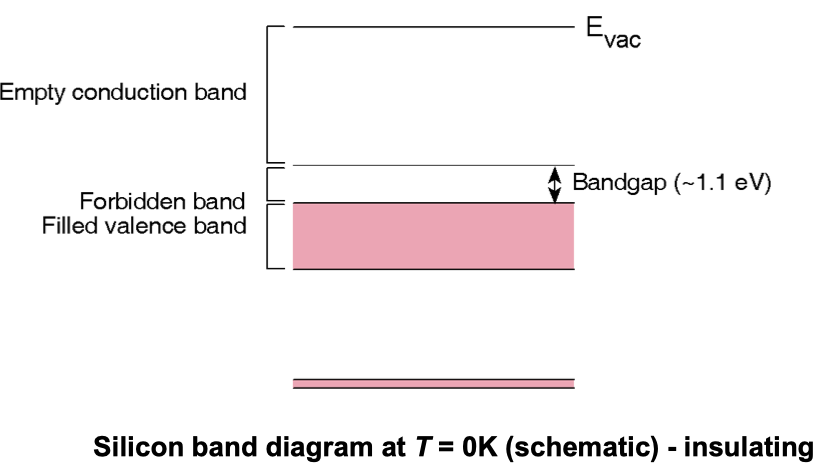
\includegraphics[width=0.75\linewidth]{image/semibandgap.png}
    \end{figure}
    Typical Bandgaps 
    \begin{table}[h!]
      \centering
      \caption{Bandgaps of selected semiconductors at 300K}
      \begin{tabular}{lc}
        \toprule
        Semiconductor & Band gap in eV at 300 K \\
        \midrule
        Silicon (Si) & 1.12 \\
        Germanium (Ge) & 0.66 \\
        Gallium Arsenide (GaAs) & 1.42 \\
        Indium Antimonide (InSb) & 0.17 \\
    
        \midrule
        \multicolumn{2}{l}{Note: Bandgap varies slightly with temperature} \\
        \midrule
        Insulator & Band gap in eV at 300 K \\
        \midrule
        Silicon Dioxide (SiO2) &  $>>$ 9 \\
        Silicon Nitride (Si3N4) &  $>>$ 5 \\
    
        \bottomrule
      \end{tabular}
    \end{table}
    \newpage
    \item Energy Band Diagrams \\
    \begin{figure}[h]
        \centering
        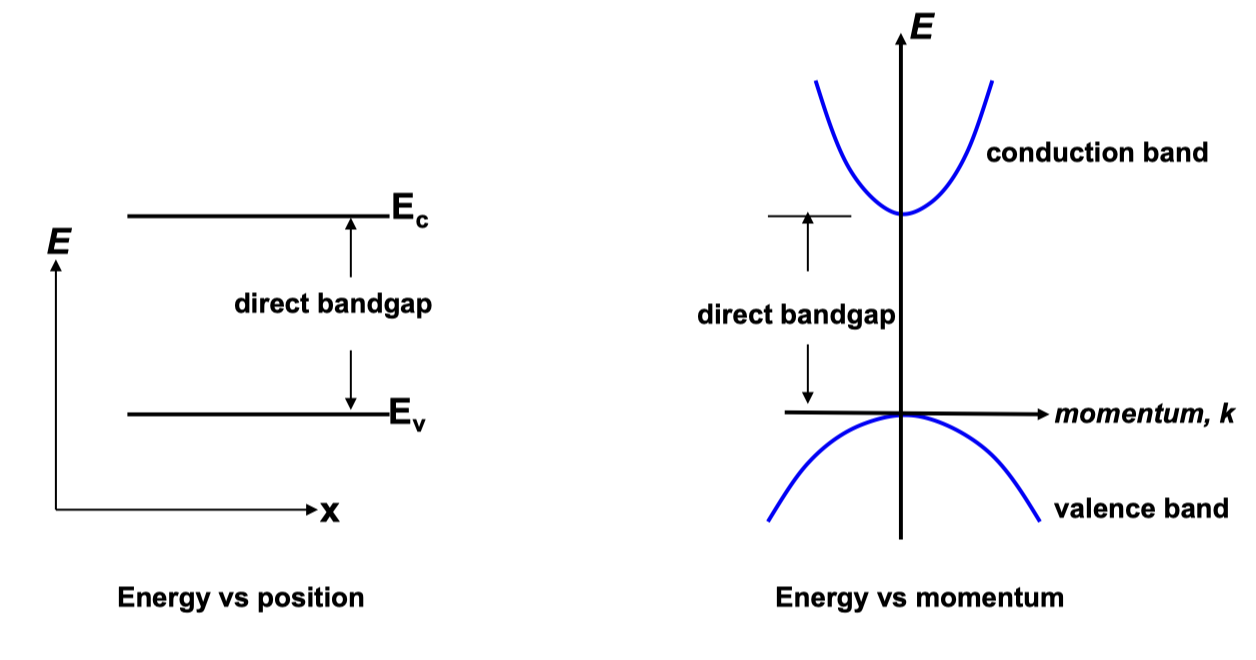
\includegraphics[width=0.75\linewidth]{image/bandgapdiagram.png}
    \end{figure}
    \item Optical Processes in Semiconductors
    \begin{figure}[h]
        \centering
        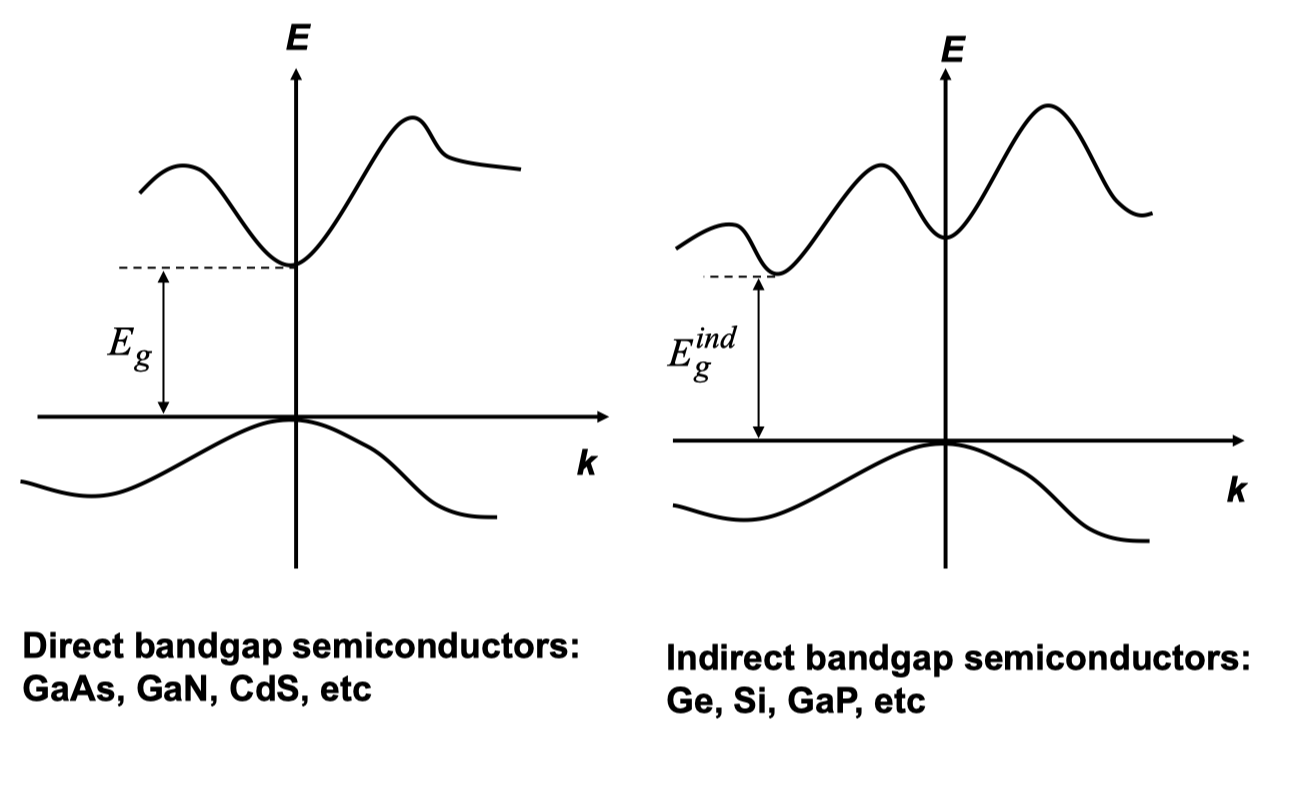
\includegraphics[width=0.75\linewidth]{image/opticalprocesssemincon.png}
    \end{figure}
    \item Direct and indirect band diagram\\
    The luminescence process involve three separae steps
    \begin{enumerate}
        \item Excitation: Electron-hole pair have to be excited by an external source of energy
        \item Thermalization: Excited e-h pairs relax towards quasi-thermal-equilibrium distributions via emitting phonon energy (lattice vibration).
        \item Recombination: The thermalized e-h pairs recombine radiatively to produce the emission of photon energy = $E_g$. Fixed $E_g$ $\rightarrow$ fixed wavelength.
    \end{enumerate}
    \item Absorption of light in a semiconductor \\
    \begin{figure}[h]
        \centering
        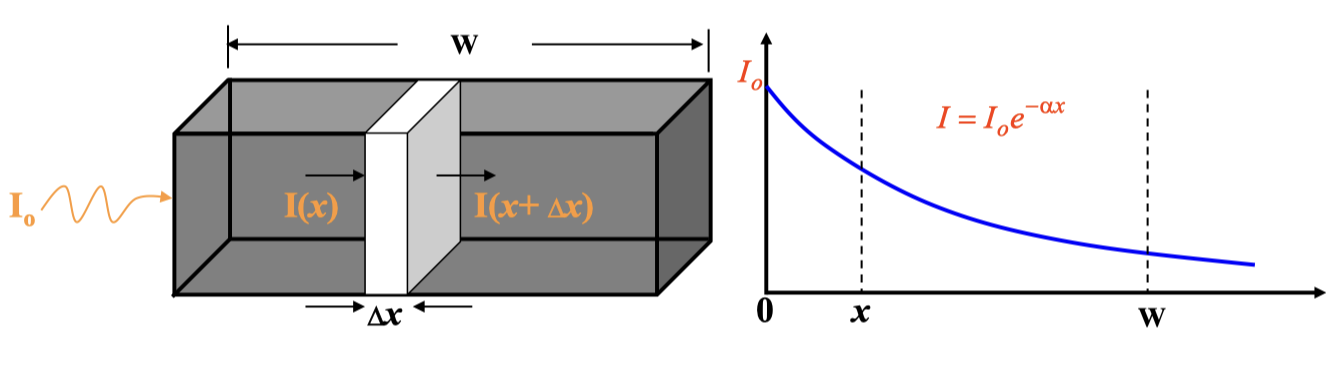
\includegraphics[width=1\linewidth]{image/absorption.png}
    \end{figure}
    \begin{equation}
        I = I_0e^{-\alpha x}
    \end{equation}
    Where $\alpha$ is the absorption coefficient which is ranged from $10^2 - 10^5$\unit{cm^{-1}}.
\end{enumerate}


\newpage
\subsection{Verilog and FPGAs}   %EE2026 starts from here
\subsubsection{First Vivado project}
\textbf{Creating project for simple Boolean logic}
\begin{enumerate}
    \item Creat a Project
    \item Select the default setting according to the board you are using, in this case is the Basys3 board which configured as [Category: General purpose; Package: cpg236; Tempreture: All remaining; Family: Artix-7; Speed: -1;]
    \item Define Module, which is for your Boolean design task, you have to add all relevent input and output in the I/O port Definitions
    \item Type out the relevent content in this design module
\end{enumerate}
\textbf{Behavioural Simulation}
\begin{enumerate}
    \item Using Project Manager to add a new simulation source
    \item Define the module name and click OK
    \item Using verilog language to create your simulation environment
    \item Example
    \begin{minted}[linenos=true]{Verilog}
module module_name(

);

    // reg is simulation for input
    reg A;    
    reg B;

    // wire is simulation for output
    wire LED1;
    wire LED2;
    wire LED3;  

    // here is the instantiation of the module to be stimulate
    simulation_module_name unit000(A, B, LED1, LED2, LED3);

    /*I would like to elaborate more on the instatiatin of the module,
    the sequence of the varibles in the bracket of unit000() should
    follow the sequence in your design source, if not you should
    approach the way of (.A(A), .B(B)) to assign values accordingly;*/
    

    initial begin
    A = 0; B = 0; #10;   // 10 is 10pico seconds
    A = 1; B = 0; #10; 
    A = 0; B = 1; #10;
    A = 1; B = 1; #10; 
    end
    
endmodule
    \end{minted}
\end{enumerate}
\textbf{Synthesis}
\begin{enumerate}
    \item Synthesis is for optimising purpose to show your logic in a more efficient way
\end{enumerate}
\textbf{Design Constrains}
\begin{enumerate}
    \item All inputs and outputs should have assign accordingly to its own constrains
    \item click Run Implementation
    \item Generate Bitstream, this step will generate a file that is in binary form to wire the logic design into the Basys3 board
    \item Open Hardware Manager
    \item Open Target
    \item Auto connect to the target.
\end{enumerate}

\newpage
\subsection{Digital Design and computer architecture}
\subsubsection{Number Systems}
\textbf{Binary-Coded Decimal}
\begin{enumerate}
    \item BCD is a code to represent ten decimal digits (0-9)
    \item Each decimal digit is reprensented by a 4-bit binary number
    \item Six number are not used in BDC
        \begin{itemize}
            \item Any addition more than 9 need to be plus a 6 $(0110)_{B}$, and the carry is 1
        \end{itemize}
    
\end{enumerate}
\subsubsection{Boolean Algebra}
\begin{enumerate}
    \item Distributive Law
    \[A + (B \cdot C)=(A+B)\cdot(A+C)\]
    \item Consensus Law
    \[AB + \bar{A}C+BC=AB+\bar{A}C\]
    \item Logical Adjacency
    \[AB+A\bar{B}=A\]
    \item Absorption Law
    \[A+A\cdot B=A\]
    \[A+\bar{A} \cdot B=A+B\]
    \item De Morgan's Law
    \[\overline{A+B}=\bar{A} \cdot \bar{B}\]
    \item Simplifying Using Boolean algebra laws
    \begin{itemize}
        \item Using Absorption Law, Logical Adjacency and Consensus Law sequencialy to obtained the simplest expression
    \end{itemize}
\end{enumerate}

\subsubsection{SOP and POS}
\begin{enumerate}
    \item \textbf{Minterm} is a product term that contains all variables in the function
    \item \textbf{Maxterm} is a sum term that contains all variables in the function
    \item \textbf{Canonical Form} is term expressed either by CSOP or CPOS
    \item SOP $\rightarrow$ Sum of Products
    \begin{itemize}
        \item If any product in SOP is \textbf{1}, the function is \textbf{1}. Otherwise is \textbf{0}
        \item CSOP only includes the terms that outcome is \textbf{1}
    \end{itemize}
    \item POS $\rightarrow$ Product of Sum
        \begin{itemize}
            \item If any sum in POS is \textbf{0}, the function is \textbf{0}. Otherwise is \textbf{1}
            \item CPOS only includes the terms that outcome is \textbf{0}
        \end{itemize}
\end{enumerate}

\subsubsection{Postive and Negative Logic}
If a logic is said to be positive or negative, they should follow the following rules
\begin{table}[h]
    \centering
    \begin{tabular}{|c|c|c|}
        \hline
        Voltage level & Positive logic value& Negative logic value \\
        \hline
        H & 1 & 0\\
        \hline
        L & 0 & 1\\
        \hline
    \end{tabular}
\end{table}

\subsubsection{Sequential Circuits}
\textbf{Synchronous and Asynchronous} \\
A \textbf{Sequential} logic circuits is said to be Synchronous is responded to inputs at discrete time instants governed by a clock input. Synchronous logic circuits need a clock. \\
An \textbf{Asynchronous} circuits responds whenever input signals change. No need clock\\
\\
\textbf{SR Flip-flop} \\
SR latch is the simplest circuit that contains memory, S is stand for set and R is stand for reset.
\begin{table}[h]
    \centering
    \begin{tabular}{|c|c|c|}
    \hline
         S & R & Output  \\
         \hline
         0 & 0 & \textcolor{red}{Hold} \\
         \hline
         0 & 1 & Q=0 \\
         \hline
         1 & 0 & Q=1 \\
         \hline
    \end{tabular}
    \caption{Truth table for SR FF}
\end{table}

\subsubsection{Linear Feedback Shift Register}




\newpage

\subsection{Signal and Systems}
\subsubsection{Classification of Signals}   
\begin{enumerate}
    \item Unit Step Function
    \begin{equation}
    u(t) = 
        \begin{cases}
             & \text{1; t $\geq$ 0}\\
             & \text{0: t $\leq$ 0}\\
        \end{cases}
    \end{equation}
    \begin{figure}[h]
        \centering
        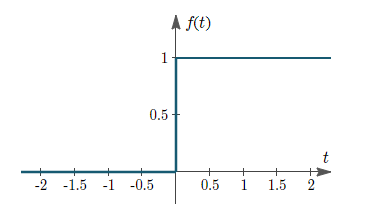
\includegraphics[width=0.6\textwidth]{image/image.png}
        \label{fig:enter-label}
    \end{figure}
    \item Sign (or Signum) function
    \begin{equation}
    sgn(t) = 
        \begin{cases}
            & +1; t \geq 0 \\
            & -1; t < 0
        \end{cases}
    \end{equation}
    \begin{figure}[h]
        \centering
        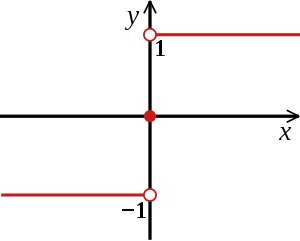
\includegraphics[width=0.5\textwidth, height=4cm]{image/Signum_function.svg.png}
        \label{fig:enter-label}
    \end{figure}
    \newpage    
    \item Rectangle Function
    \begin{equation}
    rect(\frac{t}{T}) = 
        \begin{cases}
            & 1; \frac{T}{2}\leq t < \frac{T}{2} \\
            & 0; \text{elsewhere}
        \end{cases}
    \end{equation}
    \begin{figure}[h]
        \centering
        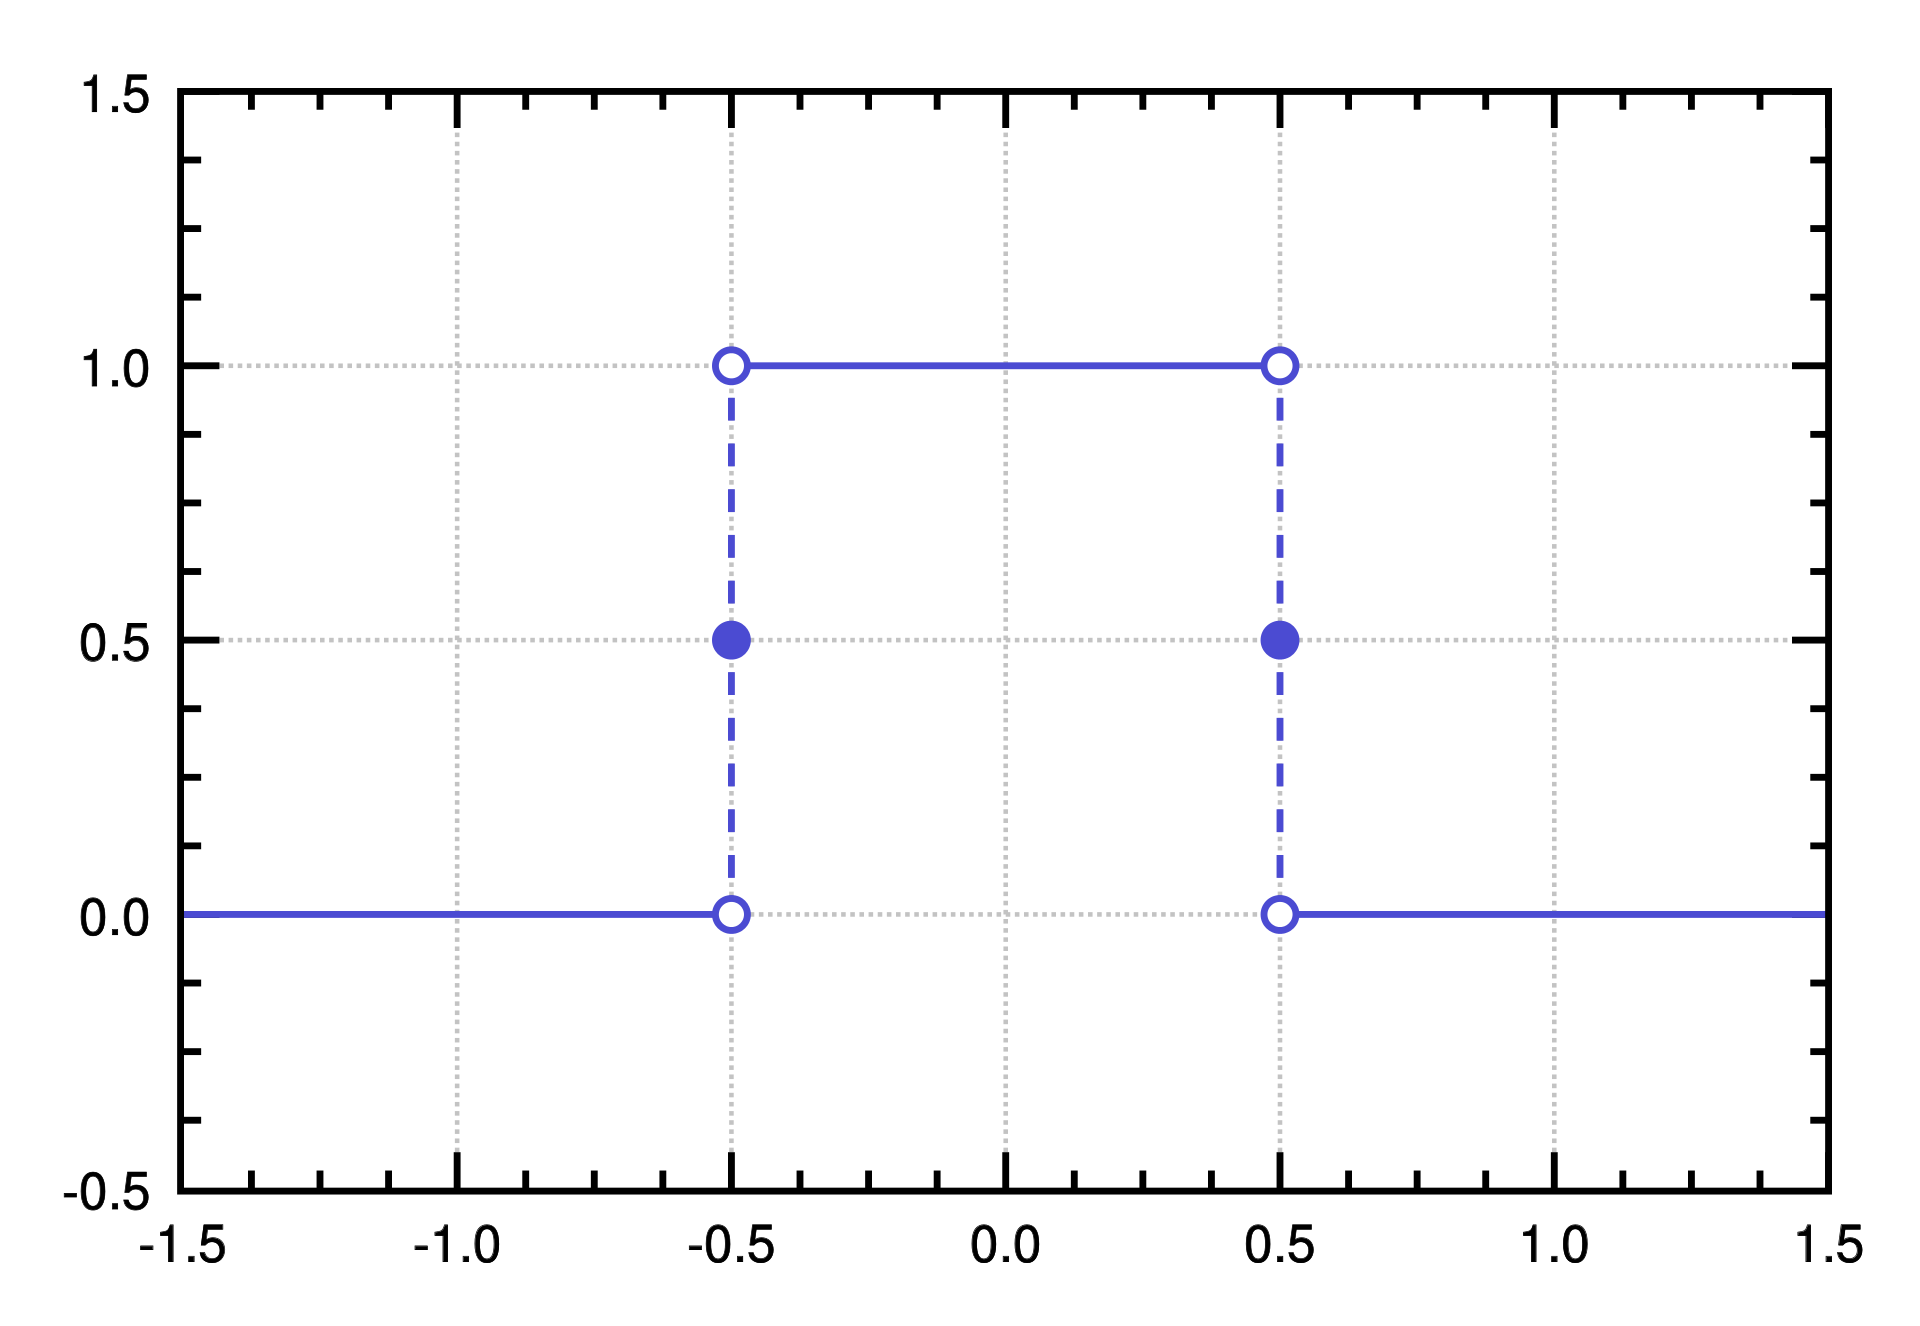
\includegraphics[width=0.6\textwidth]{image/1920px-Rectangular_function.svg.png}
        \label{fig:enter-label}
    \end{figure}
    \item Triangle function
    \begin{equation}
    tri(\frac{t}{T}) = 
        \begin{cases}
            & 1-\frac{|t|}{T};  |t|\leq T \\
            & 0;                |t|\geq T
        \end{cases}
    \end{equation}
    \begin{figure}[h]
        \centering
        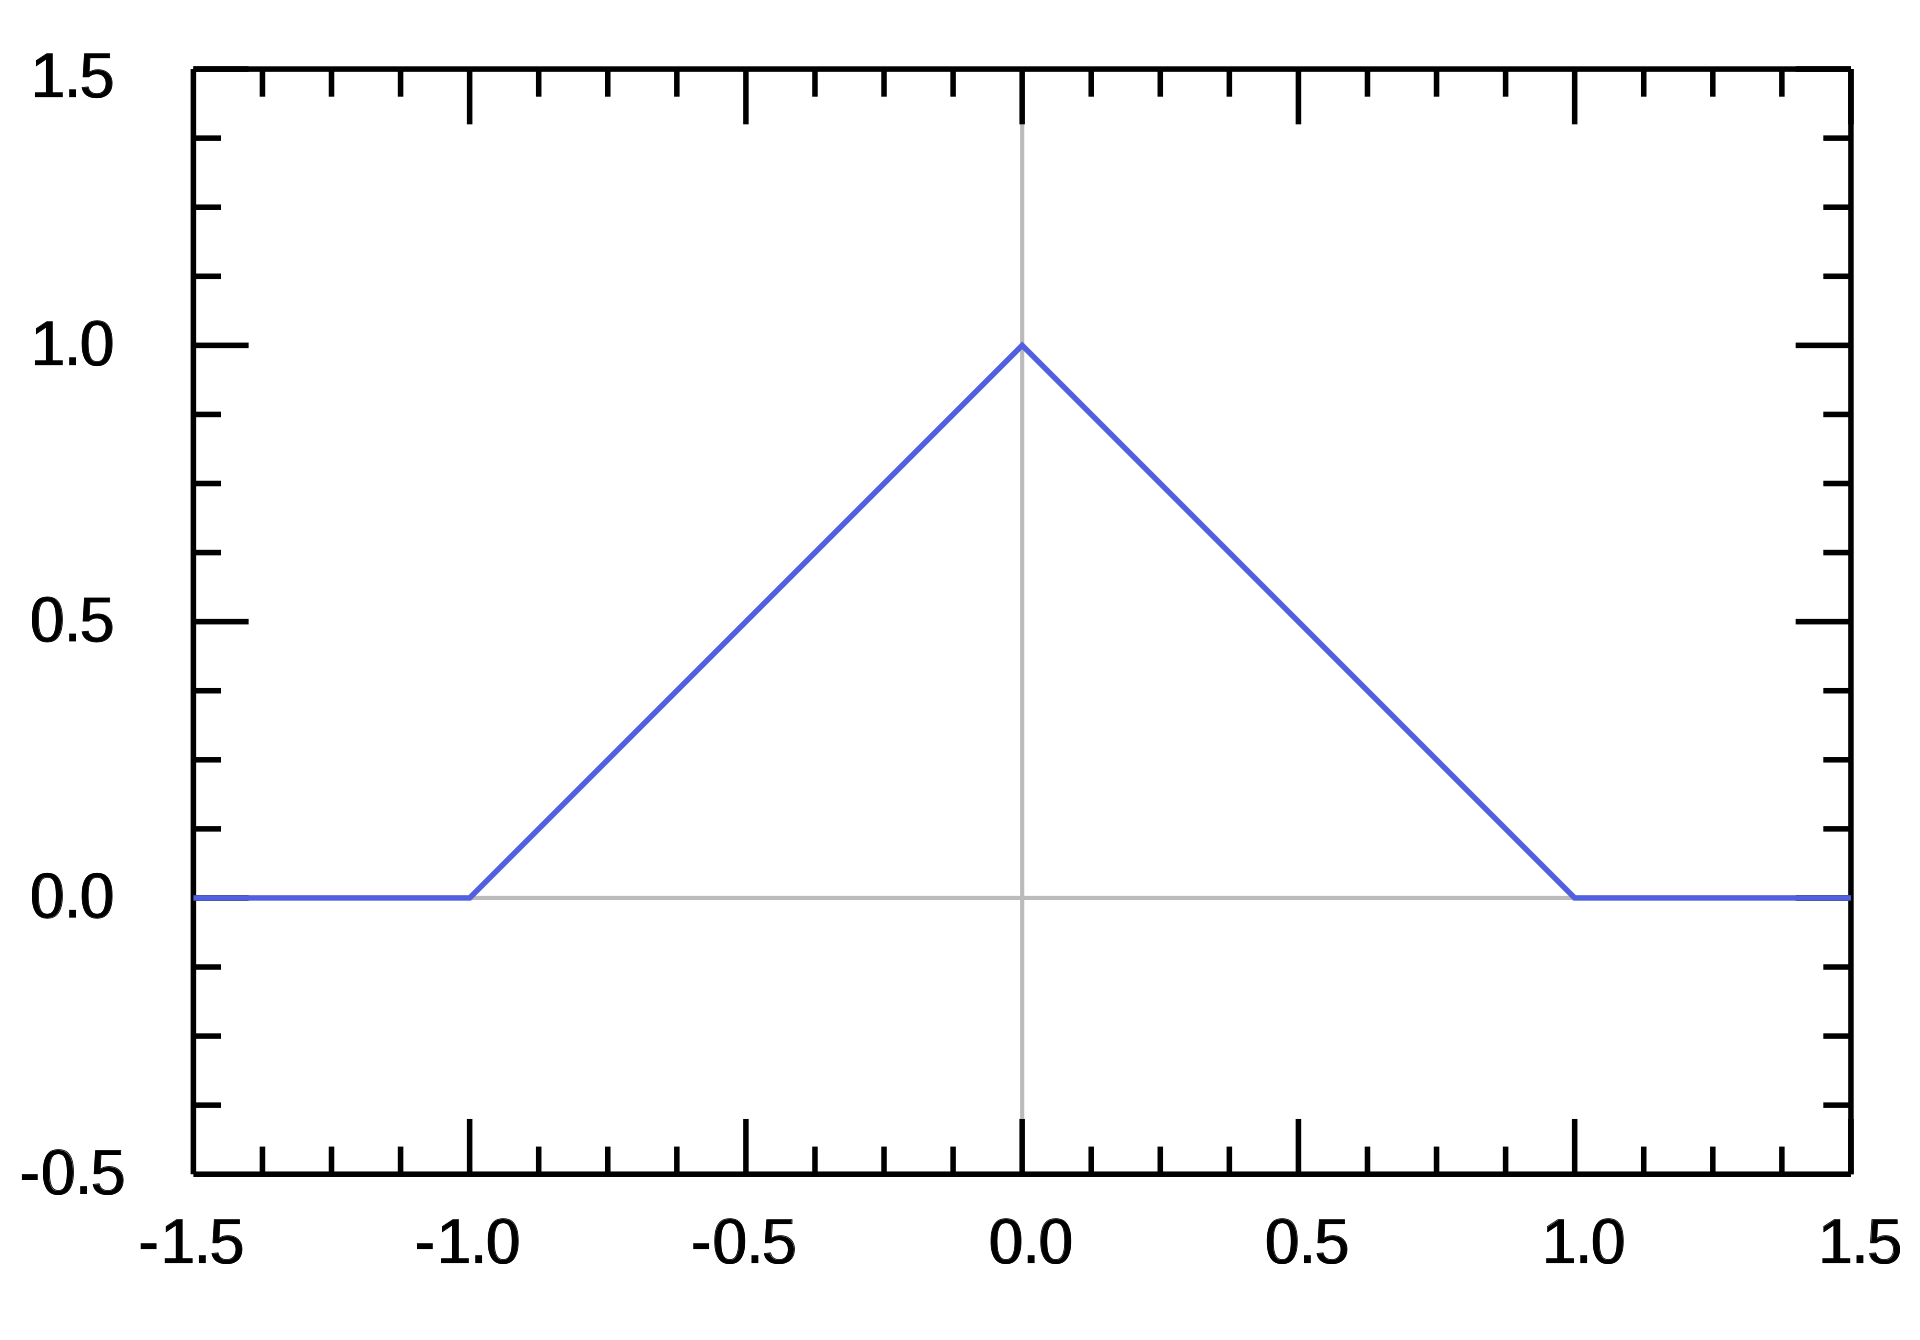
\includegraphics[width=0.6\textwidth]{image/Triangular_function.svg.png}
        \label{fig:enter-label}
    \end{figure}
    \newpage
    \item Sinc Function
    \begin{equation}
    sinc(\frac{t}{T}) = 
        \begin{cases}
            & \frac{sin(\frac{\pi t}{T})}{\frac{\pi t}{T}} ;  t \neq 0\\
            & 1 ; t \neq 0
        \end{cases}
    \end{equation}
    \begin{figure}[h]
        \centering
        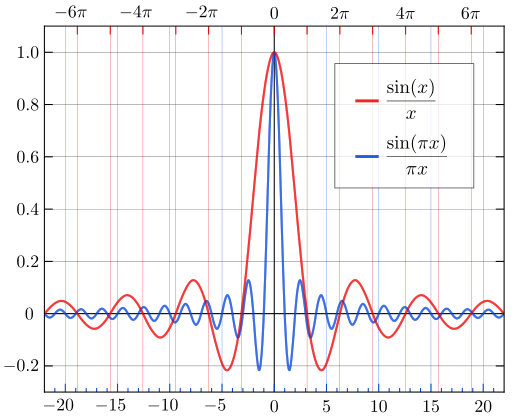
\includegraphics[width=0.6\textwidth]{image/sinc.png}
        \label{fig:enter-label}
    \end{figure}
    \\
    Take note that when calculate $sinc(x) = 0$ make sure, the $\frac{t}{T}$ in $sin(\frac{\pi t}{T})$ is integer so that $sin$ is zero, $sinc(x)$ will be zero.
    \item Two-Sided decaying exponential function
    \begin{equation}
        e^{-\alpha |t|} ; a > 0
    \end{equation}
    \begin{figure}[h]
        \centering
        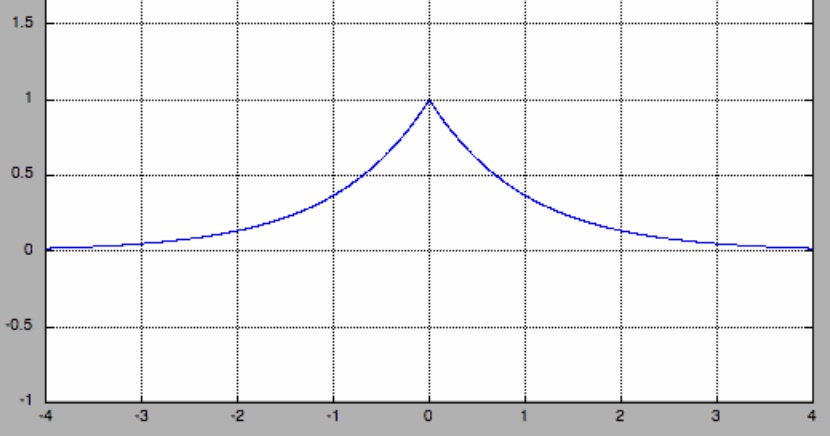
\includegraphics[width=0.6\textwidth]{image/exponential.jpg}
        \label{fig:enter-label}
    \end{figure}
    \item Right-Sided decaying exponential function
    \begin{equation}
        e^{-\alpha t}u(t) = 
        \begin{cases}
            & e^{-\alpha t} ; t \geq 0 \\
            & 0 ; t < 0 ;
        \end{cases}
    \end{equation}
    \item Sinusoidal Signals
    \begin{equation}
        x(t) = \mu cos(\omega_0t+\phi) = \frac{\mu}{2}[e^{j\omega_0t+\phi}+e^{-j(\omega_0t+\phi)}]
    \end{equation}
    \begin{equation}
        x(t) = \mu sin(\omega_0t+\phi) = \frac{\mu}{j2}[e^{j\omega_0t+\phi}-e^{-j(\omega_0t+\phi)}]
    \end{equation}
    \begin{equation}
        x(t) = \mu e^{j(\omega_0t+\phi)} = \mu[cos(\omega_0t+\phi) + jsin(\omega_0t+\phi)]
    \end{equation}
    Where \\
    $\mu > 0$ : Magnitude \\
    $\omega_0$ : angular frequency ($rad/s$)\\
    $\phi$ : phases (radian) \\
    $\omega_0t + \phi$ : instantaneous phase \\
    Take note that it is commonly replace $\omega_0$ with $2\pi f_0$ where $f_0$ is the cyclic frequency. \\
    The fundamental period $T_0$ is given by \[T_0 = \frac{2\pi}{\omega_0} = \frac{1}{f_0}\]
\end{enumerate}

\subsubsection{Time-domain Operations and Dirac Impulse}
\begin{enumerate}
    \item Time-scaling, time-shifting \\
    Lets say we have a signal $x(t)$, for $y(t) = \alpha x(\gamma t - \beta)$, where $\alpha$ is time-scaling factor and $\beta$ is time-shifting factor. To draw the signal $y(t)$, all y-coordinates should times $\alpha$ and all x-coordinates should plus $\beta$. The $\gamma$ is a stretching factor that all x-coordinates will be stretched by times $\frac{1}{\gamma}$.  
    \item Sum of two signals \\
    Given two signals to sum up. You should add all corresponding y-coordinates of each signal's 
    x-coordinates to form your new y-coordinates. 
    \newpage
    For example:
    \begin{figure}[h]
        \centering
        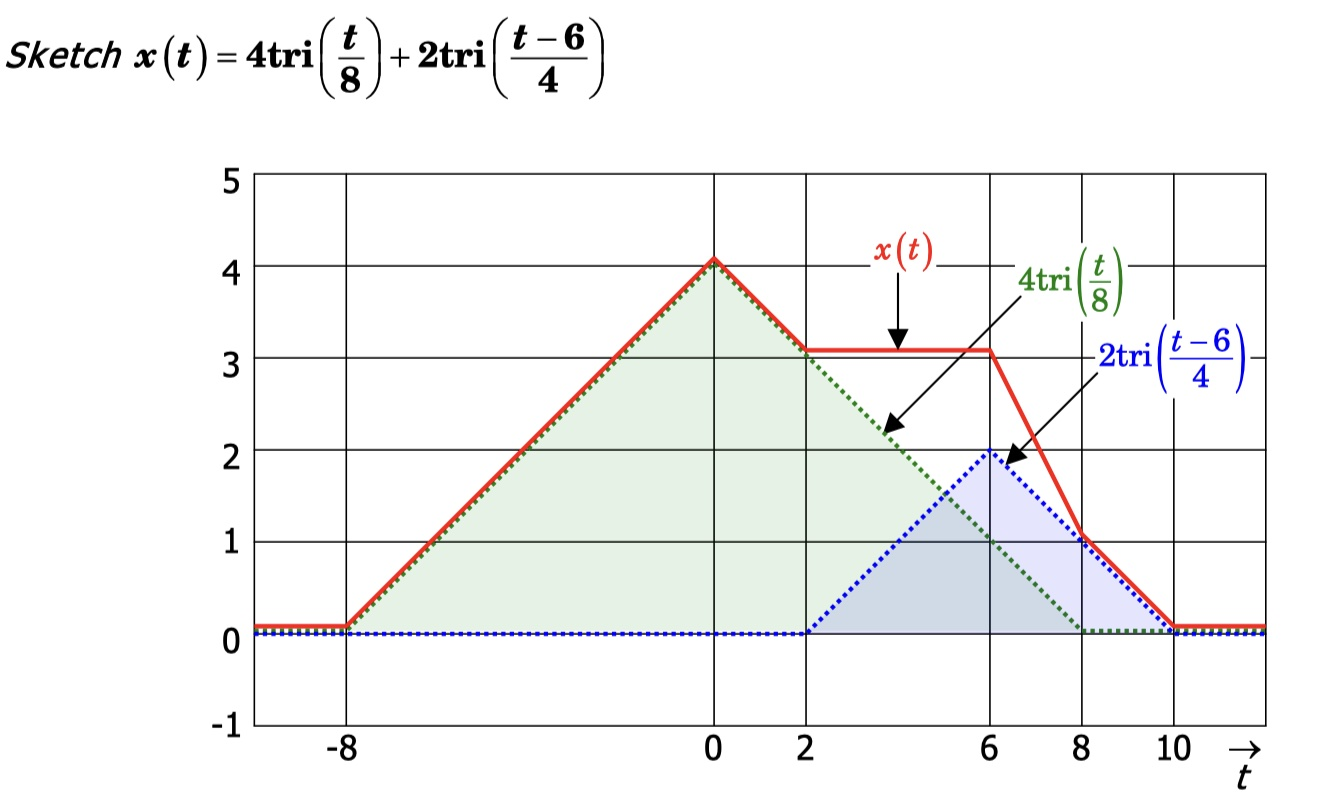
\includegraphics[width=1\textwidth]{image/triangle_add_example.jpg}
        \label{fig:enter-label}
    \end{figure}
    \item Multiplication of two signals
    \begin{figure}[h]
        \centering
        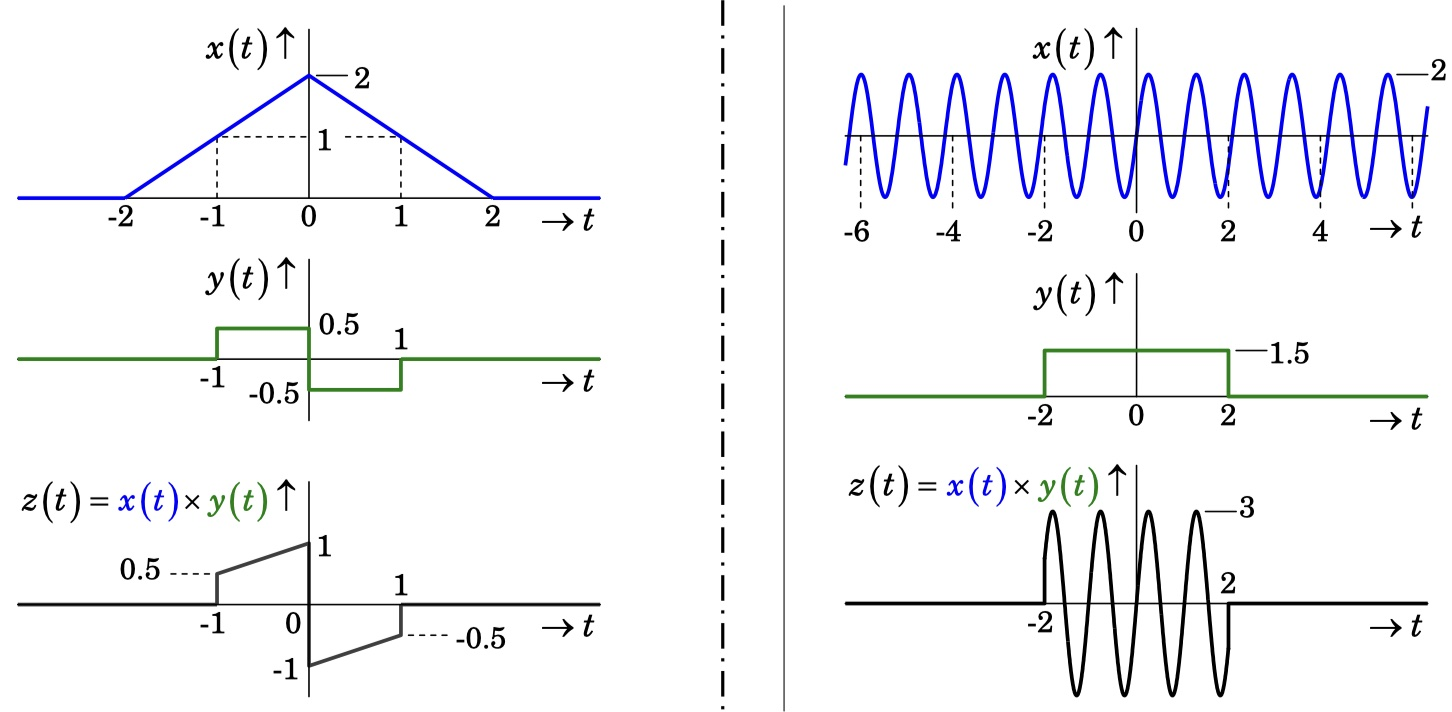
\includegraphics[width=0.9\textwidth]{image/mutiplication.jpg}
        \label{fig:enter-label}
    \end{figure}
    \item Convolution of two signals
    \begin{equation}
        x(t)*y(t) = \int^{\infty}_{\infty}x(\alpha)y(t-\alpha)d\alpha
    \end{equation}
    \newpage
    \item Dirac-$\delta$ Impulse
    \begin{itemize}
        \item The Dirac-$\delta$ function is known as \textit{unit impulse}, is defined by
        \begin{equation}
            \delta(t) = 
            \begin{cases}
                & \infty ; t = 0\\
                & 0      ; t \neq 0
            \end{cases}
        \end{equation}
    and 
    \begin{equation}
        \int^{\varepsilon}_{-\varepsilon}\delta(t)\, dt = 1 \;\; \forall\varepsilon > 0
    \end{equation}
    \item Property of $\delta(t)$ function
        \begin{enumerate}
            \item Symmetry : $\delta(t) = \delta(-t)$
            \item Sampling : $x(t)\delta(t-\lambda) = x(\lambda)\delta(t-\lambda)$
            \item Sifting : $\int^{\infty}_{-\infty}x(t)\delta(t-\lambda)dt = x(\lambda)\int^{\infty}_{-\infty}\delta(t-\lambda)dt = x(\lambda)$
            \item Replication : $x(t)*\delta(t-\lambda) = x(t-\lambda)$
        \end{enumerate}
    \end{itemize}
    \item Dirac-$\delta$ Comb Function a.k.a Sampling function
    \begin{equation}
        \sum^{\infty}_{n=-\infty}\delta(t-nT) = \dots + \delta(t+2T)+\delta(t+T)+\delta(t)+\delta(t-T)+\dots
    \end{equation}
    \begin{itemize}
        \item Replication
            \[x_p(t) = x(t)*\sum_{n}\delta(t-nT_p) = \sum_n x(t- nT_p)\]
        \item Sampling
            \[x_s(t) = x(t)\times\sum_n\delta(t-nT_s)=\sum_n x(nT_s)\delta(t - nT_s)\]
    \end{itemize}
\end{enumerate}

\subsubsection{Energy Signal and Power Signal}
\begin{enumerate}
    \item Energy Signals
    \begin{itemize}
        \item The total energy of a signal is defined as 
        \[E = \int^{\infty}_{-\infty}|x(t)|^2dt\]
        \item $x(t)$ is said to be an energy signal if $0<E<\infty$.
    \end{itemize}
    \item Power Signal
    \begin{itemize}
        \item The Average Power of a signal is defined as
        \[P = \lim_{\tau\rightarrow\infty}\frac{1}{2\tau}\int^{\tau}_{-\tau}|x(t)|^2dt\]
        \item $x(t)$ is said to be a power signal if $0<P<\infty$.
    \end{itemize}
\end{enumerate}

\subsubsection{Discrete-Frequency Spectrum}
\begin{enumerate}
    \item Spectrum of Sinusoid \\
    A spectrum of complex sinusoidal signal can be represented by 
    \[ \tilde{x(t)} = \mu e^{j(2\pi f_0t + \phi)} = \mu e^{j\phi}\times e^{j2\pi f_0 t}\]
    From this, you can draw your Magnitude spectrum and Phase spectrum. \\
    For example, 
    \begin{figure}[h]
        \centering
        \includegraphics[width=0.9\textwidth]{image/magnitude_example.jpg}
        \label{fig:enter-label}
    \end{figure}
    \item Fourier Series \\
    For any bounded periodic signal, $x_p(t)$, with period $T_p$ can be represented by a sum of harmonically related complex sinusoidal.
    \begin{equation}
        x_p(t) = \sum^{\infty}_{k=-\infty}c_k e^{j2\pi k \frac{t}{T_p}} = \sum^{\infty}_{k=-\infty}c_k e^{j2\pi kf_p t}
    \end{equation}
    where $f_p = \frac{1}{T_p}$ is the fundamental frequency of $x_p(t)$, and $kf_p$ is the $k^{th}$ harmonic of $f_p$. \\
    $c_k$ are called \textit{Fourier series coefficients} of $x_p(t)$. \\
    The function to determine $c_k$ are given by
    \begin{equation}
        c_k = \frac{1}{T_p}\int^{t_0+T_p}_{t_0}x_p(t)e^{-j2\pi k \frac{t}{T_p}}dt, \; k=0,\pm1, \pm2, \dots
    \end{equation}
    \item Trigonometric Fourier Series
    \begin{equation}
        x_p(t) = a_0 + 2\sum^{\infty}_{k=1}[a_k cos(2\pi k \frac{t}{T_p})+b_ksin(2\pi k \frac{t}{T_p})]
    \end{equation}
    where $a_k$ and $b_k$ are given by
    \[a_k = \frac{1}{T_p}\int^{t_0+T_p}_{t_0}x_p(t)cos(2\pi k \frac{t}{T_p}); \; k > 0\]
    \[b_k = \frac{1}{T_p}\int^{t_0+T_p}_{t_0}x_p(t)sin(2\pi k \frac{t}{T_p}); \; k > 0\]
\end{enumerate}
\subsubsection{Continuous-Frequency Spectrum} 
The Fourier Series expansion for a aperiodic signal does not exist. In this case, we make use of \textit{Fourier Transform} to derive the spectrum of a aperiodic signal in the continuous-frequency domain, $f$ .
\begin{enumerate}
    \item Fourier Transform \\
    \begin{equation}
        X(f) = \int^{\infty}_{-\infty}x(t)e^{-j2\pi ft}dt
    \end{equation}
    The inverse of Fourier transform is given by
    \begin{equation}
        x(t) = \int^{\infty}_{-\infty}X(f)e^{j2\pi ft}df
    \end{equation}
    \item Conditions for Fourier transformation (\textbf{Dirichlet Condition})
    \begin{itemize}
        \item $x(t)$ only has finite number of maxima and minima in any finite time interval.
        \item $x(t)$ only has finite number of discontinuities in any finite time interval.
        \item $x(t)$ is absolute integrable. For e.g. $\int^{\infty}_{-\infty}|x(t)| dt < \infty$
    \end{itemize}
    Note that point 3 is satisfied by most energy signals and violated by all power signals.
    \item Property of Fourier Transform
    \begin{enumerate}
        \item Linearity
        \begin{equation}
            \alpha x_1(t)+\beta x_2(t) \Longleftrightarrow \alpha X_1(f) + \beta X_2(f)
        \end{equation}
        \item Time Scaling
        \begin{equation}
            x(\beta t) \Longleftrightarrow \frac{1}{|\beta|}X(\frac{f}{\beta})
        \end{equation}
        \item Duality
        \begin{equation}
            X(t) \Longleftrightarrow x(-f)
        \end{equation}
        \item Time Shifting
        \begin{equation}
            x(t-t_0) \Longleftrightarrow X(f)e^{-j2\pi ft_0}
        \end{equation}
        \item Frequency Shifting
        \begin{equation}
            X(f-f_0) \Longleftrightarrow x(t)e^{j2\pi f_0t}
        \end{equation}
        \item Differentiation in the Time Domain
        \begin{equation}
            \frac{d}{dx}x(t) \Longleftrightarrow j2\pi f \cdot X(f)
        \end{equation}
        \item Integration in the Time Domain
        \begin{equation}
            \int^t_{-\infty}x(\tau)d\tau \Longleftrightarrow \frac{1}{j2\pi f}X(f)+\frac{1}{2}X(0)\delta(f) 
        \end{equation}
        \item Convolution in Time Domain
        \begin{equation}
            \underbrace{\int^{\infty}_{-\infty}x_1(\alpha)x_2(t-\alpha)d\alpha}_\text{$x_1(t)*x_2(t)$}\Longleftrightarrow X_1(f)X_2(f)
        \end{equation}
        \item Multiplication in Time Domain
        \begin{equation}
            x_1(t)x_2(t)\Longleftrightarrow \underbrace{\int^{\infty}_{-\infty}X_1(\alpha)X_2(f-\alpha)d\alpha}_\text{$X_1(f)*X_2(f)$}
        \end{equation}
    \end{enumerate}
    \newpage
    \item Fourier Transform of Basic Functions
    \begin{table}[h]
        \setlength{\arrayrulewidth}{0.3mm}
        \renewcommand{\arraystretch}{1.93}
        \centering
        \begin{tabular}{|c|c|c|}
        \hline
        &   $x(t)$     & $X(f)$ \\
        \hline
        Constant & $K$ & $K\delta(t)$ \\
        \hline
        Unit Impulse & $\delta(t)$ & $1$ \\
        \hline
        Unit Step & $u(t)$ & $\displaystyle \frac{1}{2}[\delta(f) + \frac{1}{j\pi f}]$ \\
        \hline
        Sign (Signum) & $sgn(t)$ & $\displaystyle \frac{1}{j\pi f}$ \\
        \hline
        Rectangle & $rect(\frac{t}{T})$ & $Tsinc(fT)$ \\
        \hline
        Triangle & $tri(\frac{t}{T})$ & $Tsinc^2(fT)$ \\
        \hline
        Sine Cardinal & $sinc(\frac{t}{T})$ & $Trect(fT)$ \\
        \hline
        Complex Exponential & $e^{j2\pi f_0 t}$ & $\delta(f-f_0)$ \\
        \hline
        Cosine & $cos(2\pi f_0t)$ & $\displaystyle \frac{1}{2}[\delta(f-f_0)+\delta(f+f_0)]$\\
        \hline
        Sine & $sin(2\pi f_0t)$ & $\displaystyle \frac{-j}{2}[\delta(f-f_0)-\delta(f+f_0)]$\\
        \hline
        Gaussian & $\displaystyle e^{-\frac{t^2}{\alpha^2}}$ & $\displaystyle \alpha \pi^{0.5}e^{\alpha^2\pi^2f^2}$ \\
        \hline
        Comb & $\displaystyle \sum^{\infty}_{m=-\infty}\delta(t-mT)$ & $\displaystyle \frac{1}{T}\sum^{\infty}_{k=-\infty}\delta(f-\frac{k}{T})$\\
        \hline
        \end{tabular}
        \caption{Fourier Transform Table}
        \label{tab:my_label}
    \end{table}
\end{enumerate}
\subsubsection{Spectral Density and Bandwidth}
\begin{enumerate}
    \item  Energy Spectrum Density (ESD) \\
    Energy spectral density describes how the total energy of a signal is distributed in the frequency domain. The Rayleigh’s energy theorem provides us with an alternate method for computing the total energy of a signal in the frequency-domain, namely
    \begin{equation}
        E = \int^{\infty}_{-\infty}|x(t)|^2dt = \int^{\infty}_{-\infty}|X(f)|^2df \; \text{$\cdots$\textbf{Rayleigh Energy Theorem}}
    \end{equation}
    The Energy Spectrum Density is 
    \begin{equation}
        E_x(f) = |X(f)|^2
    \end{equation}
    \item Property of \textbf{ESD} 
        \begin{enumerate}
            \item $E_x(f)$ is a real function of f
            \item $E_x(f) \geq 0 \;\; \forall f$
            \item $E_x(f)$ is an even function of $f$ if $x(t)$ is real
        \end{enumerate}
    \item Power Spectrum Density (PSD) \\
    For continuous-time signals that have infinite total energy, for example power signals, it makes more sense to define a power spectral density, which describes how the average power of a signal is distributed in the frequency domain.\\
    The \textbf{Parseval power theorem} is given by
    \begin{equation}
        P = \underbrace{\lim_{W\rightarrow\infty}\frac{1}{2W}\int^W_{-W}|x(t)|^2dt}_\text{Average Power} = \int^{\infty}_{-\infty}\lim_{W\rightarrow\infty}\frac{1}{2W}|X_W(f)|^2df
    \end{equation}
    The Power Spectrum Density
    \begin{equation}
        P_x(f) = \lim_{W\rightarrow\infty}\frac{1}{2W}|X_W(f)|^2df
    \end{equation}
    \item Property of \textbf{PSD}
        \begin{enumerate}
            \item $P_x(f)$ is a real function of f
            \item $P_x(f) \geq 0 \;\; \forall f$
            \item $P_x(f)$ is an even function of $f$ if $x(t)$ is real
        \end{enumerate}
    \item PSD for Periodic Signal\\
    Given a $x_p(t)$ is periodic, the spectrum of $x_p(t)$ is given by
    \[X_p(f) = \sum^{\infty}_{k=-\infty}c_k\delta(f-kf_p)\]
    The \textbf{Power Spectrum Density of $x_p(t)$} is
    \[P_x(f) = \sum^{\infty}_{k=-\infty}|c_k|^2\delta(f-kf_p) \]
    The \textbf{Average Power of $x_p(t)$} is 
    \[P = \int^{\infty}_{-\infty}P_x(f)\;df = \sum^{\infty}_{k=-\infty}|c_k|^2\]
    \item Bandwidth
    \begin{enumerate}
        \item Lowpass Signal\\
        A signal $x(t)$ is said to be a bandlimited lowpass signal if its magnitude spectrum is concentrated around $0 Hz$ , and at the same time satisfies
        \[|X(f)| = 0 ; \; |f| > B\]
        where B is defined as the bandwidth of the signal
        \item Bandpass Signal \\
        A signal $x(t)$ is said to be a bandlimited bandpass signal if its magnitude spectrum is concentrated around a non-zero center frequency, $f_c$ , and at the same time satisfies
        \[|X(f)| = 0 ; \; ||f| -f_c|> \frac{B}{2}\]
        \item \textbf{3dB} Bandwidth \\
        The 3dB bandwidth of $x(t)$ is defined as the frequency where 
        \[X(f) = \frac{|X(0)|}{\sqrt{2}}\; or \; |X(f)| = \sqrt{X(f)X^*(f)} \; or \; \frac{E_x(f_B)}{E_x(0)} = \frac{|X(f_B)|^2}{|X(0)|^2} = \frac{1}{2}\]
        first occurs when $f$ is increased from 0 Hz
        \item \textbf{$1^{st}-null$} Bandwidth \\
        The $1^{st}$-null bandwidth of a lowpass signal $x(t)$ is defined as the frequency at which 
        \[X(f) = 0\]
        first occurs when f increased from 0 Hz
    \end{enumerate}
    \item \textbf{M\%} Energy Containment Bandwidth \\
    The M\% energy containment bandwidth, $B$, of a real energy signal is the smallest bandwidth that contains at least M\% of the total energy 
    \[\int^{f_B}_{-f_B}E_x(f)\;df = \frac{M}{100}\times E\]
    \item \textbf{M\%} Power Containment Bandwidth \\
    The M\% power containment bandwidth, $B$, of a real energy signal is the smallest bandwidth that contains at least M\% of the average signal power. The M\% power containment bandwidth, $B$, is given by $B = Kf_p$, where K is the smallest positive integer that satisfies 
    \[\sum^{K}_{k=-K}|c_k|^2\geq\frac{M}{100}\times P\]
\end{enumerate}
\newpage
\subsubsection{Classification and s-Domain Analysis}
\begin{enumerate}
    \item Laplace Transformation
        \begin{table}[h]
            \setlength{\arrayrulewidth}{0.3mm}
            \renewcommand{\arraystretch}{1.93}
            \centering
            \begin{tabular}{|c|c|c|}
            \hline
               & $f(t)$ & $\tilde{F}(s)$ \\
            \hline
            Unit Impulse & $\delta(t)$ & $1$ \\
            \hline
            Unit Step & $u(t)$ & $\displaystyle\frac{1}{s}$ \\
            \hline
            Ramp & $tu(t)$ & $\displaystyle \frac{1}{s^2}$ \\
            \hline
            $n^{th}$ order Ramp & $t^nu(t)$ & $\displaystyle \frac{n!}{s^{n+1}}$ \\
            \hline
            Damped Ramp & $\displaystyle te^{-\alpha t}u(t)$ & $\displaystyle \frac{1}{(s+\alpha)^2}$ \\
            \hline
            Exponential & $\displaystyle e^{-\alpha t}u(t)$ & $\displaystyle\frac{1}{s+\alpha}$ \\
            \hline
            Cosine & $cos(\omega_0t)u(t)$ & $\displaystyle \frac{s}{(s^2+\omega_0^2)}$\\
            \hline
            Sine & $sin(\omega_0t)u(t)$ & $\displaystyle \frac{\omega_0}{(s^2+\omega_0^2)}$\\
            \hline
            Damped Cosine & $\displaystyle e^{-\alpha t}cos(\omega_0t)u(t)$ & $\displaystyle \frac{s+\alpha}{(s+\alpha)^2+\omega_0^2}$ \\
            \hline
            Damped Sine & $\displaystyle e^{-\alpha t}sin(\omega_0t)u(t)$ & $\displaystyle \frac{\omega_0}{(s+\alpha)^2+\omega_0^2}$\\
            \hline
            \end{tabular}
            \caption{Laplace Transformation Table}
            \label{tab:my_label}
        \end{table}
    \item Property of Laplace Transformation
    \begin{enumerate}
        \item Linearity
        \[\alpha f_1(t)+\beta f_2(t) \Longleftrightarrow \alpha \tilde{F_1}(s) + \beta\Tilde{F_2}(s)\]
        \item Time Shifting
        \[f(t-t_0) \Longleftrightarrow e^{-st_0}\Tilde{F}(s)\]
        \item Shifting in the s-domain 
        \[e^{s_0t}f(t) \Longleftrightarrow \Tilde{F}(s-s_0)\]
        \item Time Scaling
        \[f(\alpha t) \Longleftrightarrow \frac{1}{|\alpha|}\Tilde{F}(\frac{s}{\alpha})\]
        \item Integration in time-domain
        \[\int^t_0f(\zeta)d\zeta \Longleftrightarrow \frac{1}{s}\Tilde{F}(s)\]
        \item Differentiation in time-domain
        \[\frac{df(t)}{dt} \Longleftrightarrow s\Tilde{F}(s)-f(0^-)\]
        \[\frac{d^nf(t)}{dt^n} \Longleftrightarrow s^n\Tilde{F}(s)-\sum^{n-1}_{k=0}s^{n-1-k}\frac{d^kf(t)}{dt^k}\bigg|_{t=0^-}\]
        \item Differentiation in s-domain
        \[-tf(t) \Longleftrightarrow \frac{d\Tilde{F}(s)}{ds}\]
        \[(-t)^nf(t) \Longleftrightarrow \frac{d^n\Tilde{F}(s)}{ds^n}\]
        \item Convolution in the time-domain
        \[\underbrace{\int^{\infty}_{-\infty}f_1(\zeta)f_2(t-\zeta)d\zeta}_\text{$f_1(t)*f_2(t)$} \Longleftrightarrow \Tilde{F_1}(s)\Tilde{F_2}(s)\]
        \item Initial value theorem
        \[f(0) = \lim_{s\rightarrow \infty}s\Tilde{F}(s)\]
        \item Final value theorem
        \[\lim_{t\rightarrow\infty}f(t) = \lim_{s\rightarrow\infty}s\Tilde{F}(s)\]
        \item Common Partial Fraction Rules
        \[\frac{px+q}{(x-a)(x-b)}, a\neq b \; \Longleftrightarrow \frac{A}{x-a}+\frac{B}{x-b}\]
        \[\frac{px+q}{(x-a)^2} \Longleftrightarrow \frac{A}{x-a}+\frac{B}{(x-a)^2}\]
        \[\frac{px^2+qx+r}{(x-a)(x-b)(x-c)} \Longleftrightarrow \frac{A}{x-a}+\frac{B}{x-b}+\frac{C}{x-c}\]
        \[\frac{px^2+qx+r}{(x-a)^2(x-b)} \Longleftrightarrow \frac{A}{x-a}+\frac{B}{(x-a)^2}+\frac{C}{x-b}\]
        \[\frac{px^2+qx+r}{(x-a)(x^2+bx+C} \Longleftrightarrow \frac{A}{x-a}+\frac{Bx+C}{x^2+bx+c}\]
    \end{enumerate}
\end{enumerate}
\subsubsection{Linear Time-Invariant(LTI) Systems}
    \tikzstyle{block} = [draw, fill=white, rectangle, 
        minimum height=3em, minimum width=6em]
    \tikzstyle{sum} = [draw, fill=white, circle, node distance=1cm]
    \tikzstyle{input} = [coordinate]
    \tikzstyle{output} = [coordinate]
    \tikzstyle{pinstyle} = [pin edge={to-,thin,black}]
\begin{enumerate}
    \item Impulse Response\\
    The impulse response , $h(t)$, of a continuous-time LTI system is defined as the response (or output) of the system when the input is a unit impulse, $\delta(t)$ ,
    \begin{center}
        \begin{tikzpicture}[auto, node distance=2cm,>=latex']
            \node [](a){$\delta(t)$};
            \node[block, right of=a](System){LTI system \textbf{T}};
            \node[right of=System](b){$h(t)$};
            \draw [draw,->] (a) -- (System);
            \draw [draw,->](System)--(b);
        \end{tikzpicture}
    \end{center}
    where $h(t)=\textbf{T}[\delta(t)]$, now suppose an input $x(t)$ 
    \begin{center}
        \begin{tikzpicture}[auto, node distance=2cm,>=latex']
            \node [](a){$x(t)$};
            \node[block, right of=a](System){LTI system $h(t)$};
            \node[right of=System, node distance = 3cm](b){$y(t)=x(t)*h(t)$};
            \draw [draw,->] (a) -- (System);
            \draw [draw,->](System)--(b);
        \end{tikzpicture}
    \end{center}
    \item Step Response \\
    Suppose the input to the system is a unit step function, $u(t)$.
    \[\underbrace{u(t)=\int^y_{-\infty}\delta(\tau)d\tau}_\text{Unit Step}\rightarrow\boxed{h(t)}\rightarrow \underbrace{o(t)=\int^t_{-\infty}h(\tau)d\tau}_\text{Step Response}\]
    \item Frequency Response\\
    The frequency response $H(f)$ of a LTI system is defined as the Fourier transform of the system impulse response $h(t)$, namely
    \[H(f) = \mathscr{F}\{h(t)\}=\int^{\infty}_{-\infty}h(t)e^{-j2\pi ft}dt\]
    As such, the relationship between the input and output of the LTI system can be derived as
    \[X(f)\rightarrow\boxed{\text{LTI system,}\;H(f)}\rightarrow Y(f) = X(f)\cdot H(f)\]
    Since the $H(f)$ is in general a complex function of $f$, we may express it in exponential form as 
    \[H(f) = |H(f)|e^{j\angle H(f)}\]
    \item Transfer Function\\
    The transfer function $\Tilde{H}(s)$ of a LTI system is defined as the Laplace transform of the system impulse response $h(t)$ , namely
    \[\Tilde{H}(s) = \mathscr{L}\{h(t)\}=\int^{\infty}_0h(t)e^{-st}dt\]
    where $s = \sigma + j\omega$ is a complex variable.\\
    As such, the relationship between the input and output of the LTI system in s-domain can be derived as
    \[\Tilde{X}(s)\rightarrow\boxed{\text{LTI system}\;\Tilde{H}(s)}\rightarrow\Tilde{Y}(s)=\Tilde{X}(s)\cdot\Tilde{H}(s)\]
    where $\Tilde{X}(s) = \mathscr{L}\{x(t)\}$ and $\Tilde{Y}(s) = \mathscr{L}\{y(t)\}$ are the Laplace transform of the system input and output. \\
    A good technique to represent the transfer function is in its cascade form, 
    \[\Tilde{H}(s) = K\frac{(\frac{s}{z_1}+1)(\frac{s}{z_2} +1)\cdots(\frac{s}{z_n}+1)}{(\frac{s}{p_1}+1)(\frac{s}{p_2}+1)\cdots(\frac{s}{p_n}+1)}; \;\;K = \frac{b_0}{a_0}\]
    For Example, a given transfer function $\Tilde{H}(s) = \frac{s^2+3s+2}{(s^2+2s+1)(s+3)}$, the 3D plot of $|\Tilde{H}(s)|$ is shown below.\\
    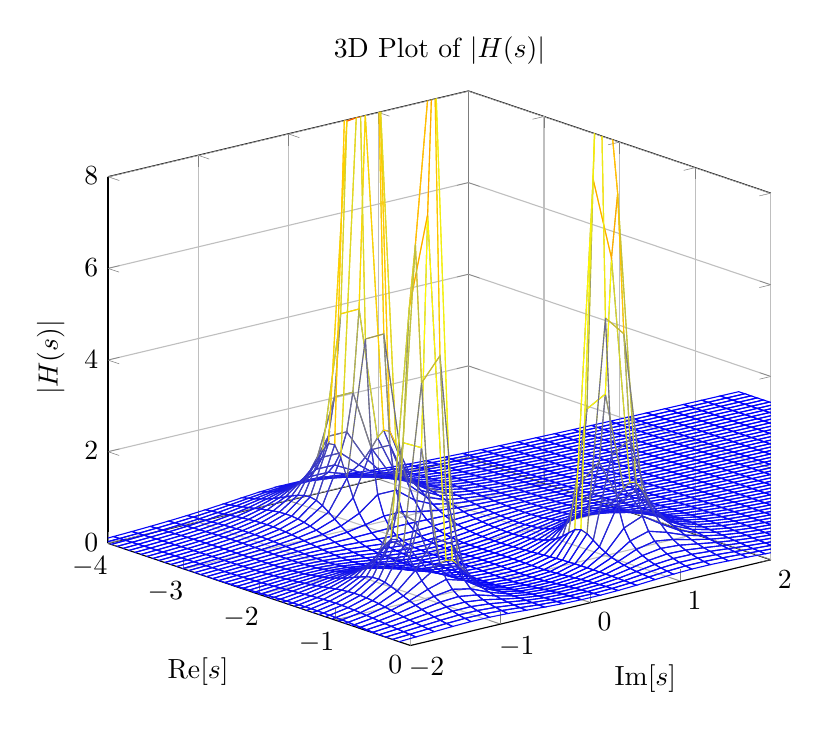
\begin{tikzpicture}
    \begin{axis}[
        view={50}{20},
        width=10cm,
        grid=major,
        xmin=-4, xmax=0,
        ymin=-2, ymax=2,
        zmin=0, zmax=8,
        xlabel={Re[$s$]},
        ylabel={Im[$s$]},
        zlabel={$|H(s)|$},
        title={3D Plot of $|H(s)|$},
        samples=50,
        domain=-4:0,
        y domain=-5:5
    ]
    \addplot3[mesh, shader=interp]
        {
            abs((x+1)*(x+1) + y*y) * abs((x+2)*(x+2) + y*y) / 
            (
                abs((x+3)*(x+3) + y*y) * 
                abs((x+1)*(x+1) + (y+1)*(y+1)) * 
                abs((x+1)*(x+1) + (y-1)*(y-1))
            )
        };
    \end{axis}
    \end{tikzpicture}
    
    \item Relationship between Transfer function and Frequency Response \\
    By substituting $s = j\omega$, we obtain
    \[\Tilde{H}(s)\Bigg|_{s=j\omega}=\Tilde{H}(j\omega)=\int^\infty_0h(t)e^{-j\omega t}dt\]
    By substituting $\omega = 2\pi f$, we obtain
    \[\Tilde{H}(j\omega)\Bigg|_{\omega=2\pi f} = \int^\infty_0h(t)e^{-j2\pi ft}dt\]
    Therefore, for a causal LTI system where $h(t) = 0$ when $t < 0$ , we have 
    \[H(f) = \Tilde{H}(j\omega)\Bigg|_{\omega = 2\pi f} = |\Tilde{H}(j\omega)|e^{j\angle \Tilde{H}(j\omega)}\]
    Thus we can conclude that
    \[x(t) = Ae^{j(\omega_0t+\psi)}\rightarrow\boxed{\Tilde{H}(j\omega)}\rightarrow y(t)=A|\Tilde{H}(j\omega_0)|e^{j(\omega_0t+\psi+\angle\Tilde{H}(j\omega_0))}\]
    \[x(t) = Acos(\omega_0t+\psi)\rightarrow\boxed{\Tilde{H}(j\omega)}\rightarrow y(t)=A|\Tilde{H}(j\omega_0)|cos(\omega_0t+\psi+\angle\Tilde{H}(j\omega_0))\]
    \[x(t) = Asin(\omega_0t+\psi)\rightarrow\boxed{\Tilde{H}(j\omega)}\rightarrow y(t)=A|\Tilde{H}(j\omega_0)|sin(\omega_0t+\psi+\angle\Tilde{H}(j\omega_0))\]
    \item System Stability \\
    Poles and Zeros : Poles are defined as the roots of the denominator polynomial of $\Tilde{H}(s)$, whenever $\Tilde{H}(\alpha) = \infty$, $\alpha$ is Pole of the system. Zeros are defined as the roots of the numerator polinomial of $\Tilde{H}(s)$, whenever $\Tilde{H}(\beta) = 0$, $\beta$ is Zero of the system.
    \begin{enumerate}
        \item BIBO Stable
        \begin{itemize}
            \item $\displaystyle\lim_{t \rightarrow \infty } h(t) = 0$
            \item All system poles lying on the left-half of s-plane.
        \end{itemize}
        \item Marginally Stable
        \begin{itemize}
            \item $\displaystyle \lim_{t \rightarrow \infty }|h(t)| \neq 0$ and $\displaystyle \lim_{t \rightarrow \infty}h(t) \neq 0$
            \item One or more system poles lying on the imaginary axis of the s-plan and no system pole lying on the right half s-plane. System poles lying on the imaginary axis must be distinct (non-repeated).
        \end{itemize}
        \item Unstable 
        \begin{itemize}
            \item $\displaystyle\lim_{t \rightarrow \infty } |h(t)| = \infty $
            \item One or more system poles lying on the right-half s-plane.
        \end{itemize}
    \end{enumerate}
\end{enumerate}
\subsubsection{First Order System}
\begin{enumerate}
    \item Differential Equation
    \begin{equation}
        T\frac{dy(t)}{dt}+y(t)=Kx(t)
    \end{equation}
    \[
        where = 
        \begin{cases}
            & x(t) : system\;input \\
            & y(t) : system\;output \\
            & K : DC\;Gain\\
            & T : time-constant
        \end{cases}
    \]
    \item Transfer Function \\
    By assuming zero initial conditions
    \begin{multline}
        TsY(s)+Y(s) = KX(s) \longrightarrow \Tilde{H}(s) = \frac{Y(s)}{X(s)}=\frac{K}{Ts+1} \\ 
    \end{multline}
    Poles: $s_1 = - \frac{1}{T}$
    \item Impulse Response $h(t)$
    \begin{equation}
        h(t) = \mathscr{L}^{-1}\{\Tilde{H}(s)\} = \frac{K}{T}e^{\frac{-t}{T}}u(t) 
    \end{equation}
    \begin{figure}[h]
        \centering
        \includegraphics[width=0.75\linewidth]{e2ba5c9507c51e791e37c061e3eef1a.png}
    \end{figure}
    \item Step Response $o(t)$
    \begin{align*}
        o(t) &=  \int^t_{-\infty}h(\tau)d\tau \\
         &= \mathscr{L}^{-1}\{\frac{1}{s}\Tilde{H}(s)\} \\
         &= K[1-e^{t\frac{t}{T}}]u(t)
    \end{align*}
    \begin{figure}[h]
        \centering
        \includegraphics[width=0.75\linewidth]{9e19b7ea507f2d6e90b842d6f5b0fac.png}
    \end{figure}
\end{enumerate}
\subsubsection{Second Order System}
\begin{enumerate}
    \item Differential Equation
    \begin{equation}
        \frac{d^2y(t)}{dt^2}+2\zeta\omega_n\frac{dy(t}{dt}+\omega_n^2y(t) = K\omega_n^2x(t)
    \end{equation}
    \[
    where = 
    \begin{cases}
        & x(t) : system\;input \\
        & y(t) : system\;output \\
        & \zeta : damping\;ratio\\
        & \omega_n : undamped\;natural\;frequency\;(when \zeta < 1) \\
        & K : DC\;Gain
    \end{cases}
    \]
    \item Transfer Function $\Tilde{H}(s)$
    \begin{multline}
        s^2Y(s)+s2\zeta\omega_nsY(s)+\omega_n^2Y(s) = K\omega_n^2X(s) \\
        \longrightarrow \Tilde{H}(s)=\frac{Y(s)}{X(s)} = \frac{K\omega_n^2}{s^2+2\zeta\omega_n s+\omega_n^2}
    \end{multline}
    Poles: $s_{1,2} = -\omega_n\zeta \pm \omega_n(1-\zeta^2)^{1/2}$ 
    \begin{itemize}
        \item $\zeta > 1 $ : $s_{1,2} = -\omega_n\zeta \pm \omega_n(1-\zeta^2)^{1/2}$ \\
        Poles are real and distinct. \\
        System is said to be \textbf{OVERDAMPED}
        \item $\zeta = 1$ : $s_{1,2} =-\omega_n$ \\
        Poles are real and repeated. \\
        System is sad to be \textbf{CRITICALLY DAMPED}
        \item $0<\zeta<1$: $s_{1,2} = -\omega_n\zeta \pm j\omega_n(1-\zeta^2)^{1/2}$ \\
        Poles are a complex conjugate pair. \\
        System is said to be \textbf{UNDERDAMPED}
        \item $\zeta = 0$ : $s_{1,2} =-j\omega_n$ \\
        Poles are pure-imaginary conjugate pair. \\
        System is said to be \textbf{UNDAMPED}
    \end{itemize}
    \item Impulse Response and Step Response
    \begin{enumerate}
        \item Overdamped System ($\zeta > 1$)
    \end{enumerate}


\newpage
\end{enumerate}
\subsection{Feedback Control Systems}
\subsubsection{Review of Signal and Systems}
\begin{enumerate}
    \item Elementary Signals. \\
    Please refer basic signals in the Chapter \textbf{Signal and Systems}. \\
    Complex Exponential function $Ae^{zt}$, where $z = \sigma + j\omega$.
    \begin{align*}
        y(t) &= Ae^{(\sigma+j\omega)t} = Ae^{\sigma t}e^{j\omega t} \\
        &= Ae^{\sigma t}[\cos(\omega t) + j\sin(\omega t)] \\
        \Re\{Ae^{zt}\} &= Ae^{\sigma t}\cos(\omega t) \\
        \Im\{Ae^{zt}\} &= Ae^{\sigma t}\sin(\omega t)
    \end{align*}
    Note that that when $\sigma < 0$, the signal exponential damped.
    \item Interconnection of systems
    \begin{enumerate}
        \item cascade (or series): $\displaystyle y = G(Fu) = GFu$ \\
        \begin{center}
        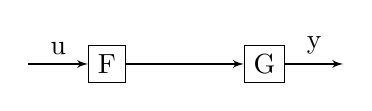
\begin{tikzpicture}[auto, node distance=2cm,>=latex']
            \node [draw, rectangle] (block1) {F};
            \node [draw, rectangle, right of=block1] (block2) {G};
            \draw [->] (-1,0) -- node[name=u] {u} (block1);
            \draw [->] (block1) -- (block2);
            \draw [->] (block2) -- node[name=y] {y} (3,0);
        \end{tikzpicture}
        \end{center}
        \item sum (or parallel) : $\displaystyle y = Fu + Gu$
        \begin{center}
            \includegraphics[width=0.5\linewidth]{image/sum.png}
        \end{center}
        \item Feedback: $\displaystyle y = F(u-Gy)$
        \begin{center}
            \includegraphics[width=0.45\linewidth]{image/feedback.png}
        \end{center}
    \end{enumerate}
    \item System Models
    \begin{enumerate}
        \item Electrical Circuits
        \begin{enumerate}
            \item Resistor: $\displaystyle v_R(t) = Ri_R(t)$
            \item Capacitor: $\displaystyle v_C(t) = \frac{1}{C}\int_0^{t}i_C(\tau)d\tau$  \hfill $i_C(t) = C\frac{dv_C(t)}{dt}$ \\
            LT domain: $\displaystyle V_C(s) = \frac{I(s)}{sC}$ \hfill  $\displaystyle Z_C(s) = \frac{1}{sC}$
            \item Inductor: $\displaystyle v_L(t) = L\frac{di_L(t)}{dt}$ \\
            LT domain: $\displaystyle V_L(s) = sLI(s)$ \hfill $\displaystyle Z_L(s) = sL$
        \end{enumerate}
        \item Linear Motions
        \begin{enumerate}
            \item Mass: $\displaystyle f(t) = M \frac{d^2x(t)}{dt}$
            \item Spring: $\displaystyle f(t) = Kx(t)$
            \item Damper: $\displaystyle f(t) = f_v\frac{dx(t)}{dt}$
        \end{enumerate}
        \item Angular Motions
        \begin{enumerate}
            \item Inertia: $\displaystyle T(t) = J\frac{d^2\theta(t)}{dt}$
            \item Spring: $\displaystyle T(t) = K\theta(t)$
            \item Damper: $\displaystyle T(t) = D\frac{d\theta(t)}{dt}$
        \end{enumerate}
    \end{enumerate}
    \item RC Circuit
    \begin{center}
        \begin{circuitikz} [american]
            \draw
            (0,0) to[V, v<=$v$] (0,2)
            to[R, l=$R$, i>^=$i$] (3,2)
            to[C, l=$C$, v<=$v_c$] (3,0) 
            to[closing switch](0,0);
        \end{circuitikz}
    \end{center}
    \begin{itemize}
        \item From the graph we can see the KVL yield: $\displaystyle v_R(t) + v_C(t) = v(t)$ 
        \item $\displaystyle Ri(t) + v_C(t) = v(t)$ 
        \item Since $\displaystyle v_C(t) = \frac{1}{C} \int i(\tau)d\tau$ or $\displaystyle i(t) = C\frac{dv_C(t)}{dt}$
        \item We have, $\displaystyle RC\frac{dv_C(t)}{dt} + v_C(t) = v(t)$ 
        \item Solving the first order equation, we have : 
        \item $\displaystyle v_c(t) = (v_c(0) - V)e^{-\frac{t}{RC}} + V$
    \end{itemize}
\end{enumerate}

\subsubsection{Review of Laplace Transform and Transfer Function}
\begin{enumerate}
\item  Why Laplace Transformation? \\
It converts integral and differential equations into algebraic equations.\\
\[
\begin{array}{|c|c||c|c|}
\hline
f(t) & F(s) & f(t) & F(s) \\
\hline
\delta(t) & 1 & \sin(bt) & \dfrac{b}{s^2+b^2} \\
U(t) & \dfrac{1}{s} & \cos(bt) & \dfrac{s}{s^2+b^2} \\
t & \dfrac{1}{s^2} & e^{-at} \sin(bt) & \dfrac{b}{(s+a)^2+b^2} \\
t^k & \dfrac{k!}{s^{k+1}} & e^{-at} \cos(bt) & \dfrac{s+a}{(s+a)^2+b^2} \\
e^{-at} & \dfrac{1}{s+a} & & \\
te^{-at} & \dfrac{1}{(s+a)^2} & & \\
\dfrac{1}{(k-1)!}t^{k-1}e^{-at} & \dfrac{1}{(s+a)^k} & & \\
\hline
\end{array}
\]
\item Derivative of LT \\
For higher order derivative: 
\[\displaystyle \mathscr{L}\{f^n(t)\} = s^n F(s) - \sum_{k=0}^{n-1} s^{n-1-k} f^k(0^-)\]
\item Integral of LT \\
Given $\displaystyle g(t) = \int_0^t f(\tau)d\tau$ then $\displaystyle G(s) = \frac{1}{s}F(s)$
\item Derivative of Transform Multiplication by time
\[F'(s) = \mathcal{L}\{-tf(t)\}\]
\[\frac{d^n}{ds^n}F(s) = (-1)^n \mathcal{L}\{t^n f(t)\}\]
For example : 
\[\mathcal{L}\{t\sin\omega t\} = -\frac{d}{ds} \left( \frac{\omega}{s^2 + \omega^2} \right) = \frac{2\omega s}{(s^2 + \omega^2)^2}
\]
\newpage
\item Other Properties of Laplace Transform
    \begin{table}[h]
    \begin{center}
    \begin{tabular}{|c|c|c|}
    \hline
    \textbf{Time Function} & \textbf{Laplace Transform} & \textbf{Comments} \\ \hline
    $\alpha f(t) + \beta g(t)$ & $\alpha F(s) + \beta G(s)$ &  Superposition \\ \hline
    $f(t - t_0)$ & $e^{-st_0}F(s)$ & Time delay $(t_0 \geq 0)$ \\ \hline
    $f(at)$ & $\displaystyle \frac{1}{|a|}F\left(\frac{s}{a}\right)$ & Time scaling  \\ \hline
    $e^{-at}f(t)$ & $F(s + a)$ & Shift in frequency \\ \hline
    $f^n(t)$ & $\displaystyle s^n F(s) - \sum_{k=0}^{n-1}s^{n-1-k}f^{(k)}(0^-)$ & Differentiation \\ \hline
    $\int_{0}^{t} f(\tau)d\tau$ & $\frac{1}{s}F(s)$ & Integration \\ \hline
    $f(t) * g(t)$ & $F(s)G(s)$ & Convolution \\ \hline
    $tf(t)$ & $-\frac{d}{ds}F(s)$ & Multiplication by time \\ \hline
    $f(0+)$ & $\displaystyle \lim_{s\to\infty} sF(s)$ & Initial value theorem \\ \hline
    $\displaystyle \lim_{t\to\infty} f(t)$ & $\displaystyle \lim_{s\to0} sF(s)$ & Final value theorem \\ \hline
    \end{tabular}
    \end{center}
    \caption{Laplace Transforms and their Time Functions}
    \label{table:laplace}
    \end{table}
\item Inverse Laplace Transform\\
Steps to take:
\begin{enumerate}
    \item Simplify complicated functions using partial fractions expansion.
    \item Obtain the inverse Laplace transform, $f(t)$ using the LT table.
\end{enumerate}
\item Transfer Function \\
A transfer function $G(s)$ is the ration of the Laplace transform of the output to the Laplace transform of the input.
\begin{equation}
    G(s) = \frac{Y(s)}{U(s)}
\end{equation}
Take note that we assume all initial conditions on the system are zero.
\end{enumerate}


\subsubsection{Dynamic Response}
\textbf{Common type of responses}
\begin{enumerate}
    \item Impulse response :  relate to transfer function.
    \item Step response : relate to physical parameters in LTI systems.
    \item Sinusoidal response : relate to frequency response of the system.
\end{enumerate}
\textbf{Poles and Zeros}
\begin{enumerate}
    \item System poles are the roots of the denominator polynomial of the transfer fucntion $G(s)$.
    \item The poles of the system determine its stability properties.
    \item The poles of the system determine the natural behaviour of the system.
\end{enumerate}
\textbf{Impulse responses}
\begin{enumerate}
    \item Impulse response ... \\
    Suppose the transfer function of a LTI system is
    \[G(s) = \frac{Y(s)}{U(s)}\]
    Its impulse response is given by $u(t) = \delta(t)$ and $U(s) = 1$ then, We will have $Y(s) = G(s)$. The inverse LT gives 
    \[y(t) = \mathscr{L}^{-1}\{G(s)\}=g(t) \quad G(s) = \mathscr{L}\{\text{Impulse Response}\}\]
    \item First Order System \\
    Consider a first order system $\displaystyle G(s) = \frac{1}{s+\sigma}$. Inverse Laplace transformation gives $g(t) = e^{-\sigma t}$. \\
    The time constant of the system $\tau$ is defined as $\displaystyle \tau = \frac{1}{\sigma}$ as $\displaystyle \frac{1}{e} = 0.368$ times the initial value. \\
    Note that the shape of the system response is dominated by the shape of the \textbf{smaller pole}.
    \item Second Order System \\
    A standard $2^{nd}$ order transfer function is expressed as
    \[H(s) = \frac{K \omega_n^2}{s^2 + 2 \zeta \omega_n s + \omega_n^2} = \frac{K \omega_n}{(s + \zeta \omega_n)^2 + \omega_n^2 (1 - \zeta^2)}\]
    The impulse response is given by
    \[y_i(t) = h(t) = \frac{K \omega_n}{\sqrt{1 - \zeta^2}} e^{-\sigma t} \sin(\omega_d t)\]
    The step response is given by
    \[y_s(t) = K - \frac{K}{\sqrt{1 - \zeta^2}} e^{-\sigma t} \sin(\omega_d t + \cos^{-1}(\zeta))\]
    \item Poles position and impulse responses
    \begin{itemize}
        \item real, positive poles correspond to growing exponential terms
        \item real, negative poles correspond to decaying exponential terms
        \item a poles at $s = 0$ correspond to a constant term
        \item complex pole pairs with positive real part correspond to exponentially growing sinusoidal terms
        \item complex pole pairs with negative real part correspond to exponentially decaying sinusoidal terms
        \item pure imaginary pole pairs correspond to sinusoidal terms
        \item repeated poles yield same types of terms, multiply by powers of t
    \end{itemize}
\end{enumerate}
\textbf{Step responses}
\begin{enumerate}
    \item For a step response $\displaystyle Y_s(s) = G(s)U(s)$, $\displaystyle y_s(t) = \mathscr{L}^{-1} \left\{ \frac{G(s)}{s} \right\}$
    \item DC Gain \\
    This is the ratio of the output of a system to its input (presumed constant) after all transients have decayed. \\
    If the magnitude of a step input is $A$. We then have the \textit{Final Value Theorem} and the DC gain is
     \[K = \frac{\displaystyle \lim_{ t \to \infty} y(t)}{\displaystyle \lim_{t \to \infty} U(t)} = \frac{AG(0)}{A} = G(0)\]
    \item Integrator 
    \[y(t) = \int_{0}^{t} K_i u(\tau) d\tau\]
    where $K_i$ is known as the integration gain.\\
    The transfer function is 
    \[G(s) = \frac{Y(s)}{U(s)} = \frac{K_i}{s}\]
    The step response is 
    \[y(t) = K_i t\]
    Integrator is marginally stable as its impulse response is non-decreasing. 
    \item Differentiator 
    \[y(t) = K_d \frac{du(t)}{dt}\]
    where $K_d$ is the derivative gain. \\
    The transfer function is 
    \[G(s) = \frac{Y(s)}{U(s)} = K_ds\]
    The step response is 
    \[y(t) = K_d \delta(t)\]
    \item Transportation delay \\
    A type of time delay occurs in systems which require a finite time to move material or transmit signal from one point to another.
    \[y(t) = u(t-t_d), \quad t_d = \frac{\text{distance}}{\text{speed}}\]
    The transfer function is 
    \[G(s) = \frac{Y(s)}{U(s)} = e^{-st_d}\]
    \item First Order System \\
    The General transfer function is given by
    \[G(s) = \frac{Y(s)}{U(s)} = \frac{K}{\tau s+1}; \quad y(0)= 0\]
    where the pole is located at $\displaystyle s =- \frac{1}{\tau}$ \\
    The unit step response is given by
    \[y_s(t) = K - Ke^{-\frac{t}{\tau}}\]
    Steady-state output $= \lim_{s\rightarrow0}G(s) \times $magnitude of step.
    The time constant $\tau$ for step response is $63.2\%$ of the final value $K$. The $2\%$ settling time is $4\tau$ around $98\%$ of $K$.
    \item Second Order System
    The general transfer function is given by
    \[G(s) = \frac{Y(s)}{U(s)} = \frac{K \omega_n^2}{s^2 + 2 \zeta \omega_n s + \omega_n^2}; \quad y(0)=y'(0)=0\]
    Poles of a second order system $\displaystyle s = -\zeta \omega_n \pm \omega_n \sqrt{\zeta^2 -1}$
    \begin{itemize}
        \item $\zeta > 1$, poles are real and distinct, system is overdamped
        \item $\zeta = 1$, poles are real and equal (repeated), system is critically damped
        \item $\zeta < 1$, poles are complex conjugate, system is underdamped
    \end{itemize}
    A pair of complex poles can be defined in real and imaginary parts: $s = -\sigma \pm j\omega_d$. \\
    where $\sigma = \zeta \omega_n$ and $\omega_d = \omega_n \sqrt{1-\zeta^2}$ \\
    The step response of a second order system is given by
    \[y(t) = K \left( 1 - \frac{e^{-\sigma t}}{\sqrt{1 - \zeta^2}} \sin(\omega_d t + \phi) \right)\]
    The magnitude of real part of the pole, determine the exponential envelope. The farther to the left of the imaginary axis, the faster it will reach the steady state.\\
    The imaginary part of pole determine the frequency of the sinusoidal signal. The bigger the value of $\omega_d$, more oscillation will occur.\\
    For over and critically damped system, the behave more like first order systems. \\
    Effect of an additional zero on the system. This will lead to a huge hump in the early part of the step response function.    
\end{enumerate}
\textbf{Time domain specifications}
\begin{enumerate}
    \item Rise time, $t_r$ : the 10\% to 90\% rise time.
    \begin{equation}
        t_r \approx \frac{1.8}{\omega_n}
    \end{equation}
    \item Overshoot $M_p$ \\
    The overshoot formula is given by
    \begin{equation}
        M_p = Ke^{-\frac{\pi \zeta}{\sqrt{1-\zeta^2}}}, \quad 0\leq\zeta<1
    \end{equation}
    The percentage overshoot is given as
    \begin{equation}
        \%M_p = \frac{M_p}{y_{ss}}\times 100\% = e^{-\frac{\pi \zeta}{\sqrt{1-\zeta^2}}}\times 100\%
    \end{equation}
    \item Peak time $t_p$ : time it takes the system to reach the maximum overshoot point\\
    The peak time is given by
    \begin{equation}
        t_p = \frac{\pi}{\omega_d}
    \end{equation}
    \item Settling time $t_s$ : the time it takes the system transient to decay\\
    Measure of smallness: 1\%, 2\%, or 5\% have been used.
    \begin{equation}
        t_s = \frac{-\ln{(\text{Measure of smallness})}}{\zeta \omega_n} = \frac{4}{\sigma}
    \end{equation}
    \item Design Synthesis \\
    You should find $\omega_n,\;\sin^{-1}\zeta,\;\sigma$ and plot on your $s$-plane.
\end{enumerate}

\subsubsection{Feedback Control}




    
\end{document}